\documentclass[11pt,aspectratio=169]{beamer}
% ============================================================
% ARSPI-Net PhD Defense -- Andrew Lane, Stony Brook ECE
% Three Dives: Neuromorphic operator | Graph propagation regime | Intrinsic interpretability
% Threaded: philosophy of rigorous inquiry, null results as motivation, theory before practice.
% Target: ~50 main slides, ~28 appendix, 45 min presenting + 20 min Q&A.
% ============================================================
\usetheme{metropolis}
\metroset{numbering=fraction, progressbar=foot, sectionpage=progressbar}
\usepackage{amsmath,amssymb,amsfonts,mathtools,bm,booktabs,graphicx,xcolor}
\usepackage{tikz}
\usetikzlibrary{arrows.meta,positioning,shapes.geometric,calc,decorations.pathreplacing,backgrounds,fit}

\definecolor{sbnavy}{HTML}{1A2A4F}
\definecolor{sbteal}{HTML}{1C7293}
\definecolor{sbaccent}{HTML}{B5651D}
\definecolor{sbgrey}{HTML}{8A94A6}
\setbeamercolor{frametitle}{bg=sbnavy}
\setbeamercolor{progress bar}{fg=sbteal}
\setbeamercolor{alerted text}{fg=sbaccent}
\newcommand{\refcite}[1]{{\scriptsize\color{gray}[#1]}}
\newcommand{\srccap}[1]{{\scriptsize\color{gray}#1}}

\title{ARSPI-Net}
\subtitle{A Staged Neuromorphic Framework for Intrinsically Interpretable Clinical EEG Analysis}
\author{Andrew Lane}
\institute{Department of Electrical \& Computer Engineering \\ Stony Brook University}
\date{Doctoral Dissertation Defense \quad\textbar\quad 2026}

\begin{document}

\maketitle

% ===============================================================
\section{Part 1 --- The Engineering Problem and the Inquiry}
% ===============================================================

\begin{frame}{The epistemological problem}
  \vspace{0.6em}
  \begin{center}
    \large How do we recover latent cortical dynamics from\\
    noisy neuroelectric observations \alert{without surrendering}\\
    scientific transparency to black-box deep learning?
  \end{center}
  \vspace{1.2em}
  \begin{itemize}
    \item Accuracy without mechanism is not science.
    \item A clinician cannot act on an opaque prediction.
    \item A researcher cannot extend an unknown mechanism.
  \end{itemize}
\end{frame}

\begin{frame}{The unobserved cortical operator $\mathcal{F}$}
  \vspace{0.8em}
  \begin{align*}
    r_p(s) &= \mathcal{F}(D_p, s;\, \delta_p) &
    x_p(s) &= g(r_p(s)) + \eta
  \end{align*}
  \vspace{0.4em}
  \begin{itemize}
    \item Conventional pipelines invert $g$ --- they shortcut the physics.
    \item ARSPI-Net is an explicit dynamical model of $\mathcal{F}$.
    \item The reservoir is not a feature extractor. It is the operator.
  \end{itemize}
\end{frame}

\begin{frame}{The inverse problem}
  \vspace{0.8em}
  \begin{center}\large
    Construct $\phi:\ x_p \mapsto \hat{D}_p$
  \end{center}
  \vspace{0.8em}
  Three requirements:
  \begin{itemize}
    \item \textbf{Stability} --- robust to noise and inter-subject variation.
    \item \textbf{Interpretability} --- internal variables map to measurable
      ERP and dynamical quantities.
    \item \textbf{Clinical generalizability} --- $\hat{D}_p$ relates to
      $\delta_p$ transdiagnostically.
  \end{itemize}
  \vspace{0.6em}
  \begin{center}\color{sbnavy}\small Conventional pipelines satisfy at most one.\end{center}
\end{frame}

\begin{frame}{Why conventional pipelines miss this problem}
  \vspace{0.6em}
  \begin{itemize}
    \item \textbf{Band-power vectors} --- collapse the epoch.
    \item \textbf{Rate-coded networks} --- discard relative timing.
    \item \textbf{End-to-end deep networks} --- no inspectable intermediates.
  \end{itemize}
  \vspace{0.8em}
  \begin{center}\color{sbnavy}
    Each integrates over the dimension that \emph{is} the signal.
  \end{center}
\end{frame}

\begin{frame}{The governing question}
  \vspace{1.2em}
  \begin{center}\large\itshape
    Can hidden dynamical order be recovered\\
    from noisy neural measurements\\
    through nonlinear transformation\,?
  \end{center}
  \vspace{1.0em}
  \begin{center}
    And does it remain \alert{stable}, \alert{compressible},\\
    \alert{structurally coherent}, and\\
    \alert{interpretable in clinically meaningful terms}\,?
  \end{center}
\end{frame}

% ===============================================================
\section{Part 2 --- Architecture and Contributions}
% ===============================================================

\begin{frame}[plain]
  \vspace{-0.3cm}
  \centering
  \resizebox{0.92\paperwidth}{!}{%
  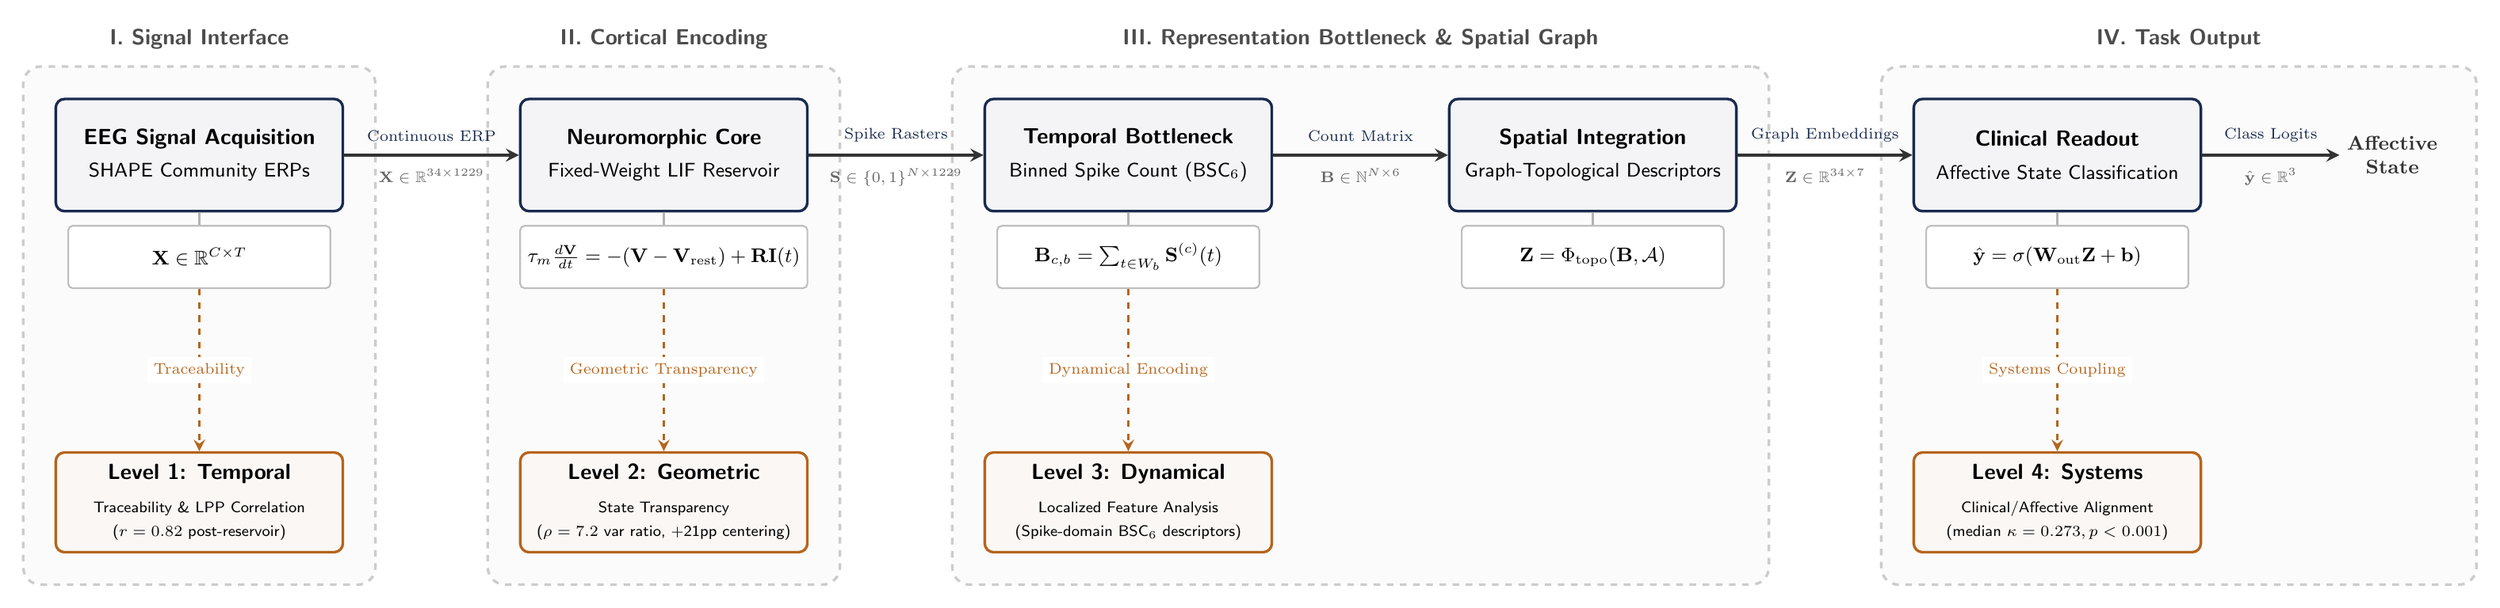
\begin{tikzpicture}[
    font=\sffamily,
    block/.style={draw=sbnavy, fill=sbnavy!5, rectangle, rounded corners=4pt, minimum width=4.6cm, minimum height=1.8cm, align=center, line width=1.2pt},
    mathblock/.style={draw=gray!50, fill=white, rectangle, rounded corners=2pt, minimum width=4.2cm, minimum height=1.0cm, align=center, font=\small, line width=0.8pt},
    taxblock/.style={draw=sbaccent, fill=sbaccent!5, rectangle, rounded corners=4pt, minimum width=4.6cm, minimum height=1.6cm, align=center, line width=1.2pt},
    arrow/.style={-stealth, draw=black!80, line width=1.6pt},
    dasharrow/.style={-stealth, dashed, draw=sbaccent, line width=1.3pt},
    container/.style={draw=gray!40, fill=gray!3, dashed, rectangle, rounded corners=8pt, inner sep=0.5cm, line width=1.2pt}
  ]
    \node[block] (input) {\textbf{EEG Signal Acquisition} \\[3pt] {\small SHAPE Community ERPs}};
    \node[mathblock, below=0.2cm of input] (m_input) {$\mathbf{X} \in \mathbb{R}^{C \times T}$};
    \draw[gray!60, line width=1pt] (input) -- (m_input);
    \node[block, right=2.8cm of input] (lsm) {\textbf{Neuromorphic Core} \\[3pt] {\small Fixed-Weight LIF Reservoir}};
    \node[mathblock, below=0.2cm of lsm] (m_lsm) {$\tau_m \frac{d\mathbf{V}}{dt} = -(\mathbf{V} - \mathbf{V}_{\text{rest}}) + \mathbf{R}\mathbf{I}(t)$};
    \draw[gray!60, line width=1pt] (lsm) -- (m_lsm);
    \node[block, right=2.8cm of lsm] (bsc) {\textbf{Temporal Bottleneck} \\[3pt] {\small Binned Spike Count ($\text{BSC}_6$)}};
    \node[mathblock, below=0.2cm of bsc] (m_bsc) {$\mathbf{B}_{c,b} = \sum_{t \in W_b} \mathbf{S}^{(c)}(t)$};
    \draw[gray!60, line width=1pt] (bsc) -- (m_bsc);
    \node[block, right=2.8cm of bsc] (gnn) {\textbf{Spatial Integration} \\[3pt] {\small Graph-Topological Descriptors}};
    \node[mathblock, below=0.2cm of gnn] (m_gnn) {$\mathbf{Z} = \Phi_{\text{topo}}(\mathbf{B}, \mathcal{A})$};
    \draw[gray!60, line width=1pt] (gnn) -- (m_gnn);
    \node[block, right=2.8cm of gnn] (readout) {\textbf{Clinical Readout} \\[3pt] {\small Affective State Classification}};
    \node[mathblock, below=0.2cm of readout] (m_read) {$\hat{\mathbf{y}} = \sigma(\mathbf{W}_{\text{out}}\mathbf{Z} + \mathbf{b})$};
    \draw[gray!60, line width=1pt] (readout) -- (m_read);
    \node[right=2.2cm of readout, font=\bfseries\small, align=center, text=black!80] (output) {Affective \\ State};
    \draw[arrow] (input) -- node[above=2pt, font=\scriptsize, text=sbnavy] {Continuous ERP} node[below=2pt, font=\scriptsize\bfseries, text=gray!80!black] {$\mathbf{X} \in \mathbb{R}^{34 \times 1229}$} (lsm);
    \draw[arrow] (lsm) -- node[above=2pt, font=\scriptsize, text=sbnavy] {Spike Rasters} node[below=2pt, font=\scriptsize\bfseries, text=gray!80!black] {$\mathbf{S} \in \{0,1\}^{N \times 1229}$} (bsc);
    \draw[arrow] (bsc) -- node[above=2pt, font=\scriptsize, text=sbnavy] {Count Matrix} node[below=2pt, font=\scriptsize\bfseries, text=gray!80!black] {$\mathbf{B} \in \mathbb{N}^{N \times 6}$} (gnn);
    \draw[arrow] (gnn) -- node[above=2pt, font=\scriptsize, text=sbnavy] {Graph Embeddings} node[below=2pt, font=\scriptsize\bfseries, text=gray!80!black] {$\mathbf{Z} \in \mathbb{R}^{34 \times 7}$} (readout);
    \draw[arrow] (readout) -- node[above=2pt, font=\scriptsize, text=sbnavy] {Class Logits} node[below=2pt, font=\scriptsize\bfseries, text=gray!80!black] {$\hat{\mathbf{y}} \in \mathbb{R}^{3}$} (output);
    \node[taxblock, below=2.6cm of m_input] (t1) {\textbf{Level 1: Temporal} \\[3pt] {\scriptsize Traceability \& LPP Correlation} \\[-1pt] {\scriptsize ($r = 0.82$ post-reservoir)}};
    \node[taxblock, below=2.6cm of m_lsm] (t2) {\textbf{Level 2: Geometric} \\[3pt] {\scriptsize State Transparency} \\[-1pt] {\scriptsize ($\rho = 7.2$ var ratio, +21pp centering)}};
    \node[taxblock, below=2.6cm of m_bsc] (t3) {\textbf{Level 3: Dynamical} \\[3pt] {\scriptsize Localized Feature Analysis} \\[-1pt] {\scriptsize (Spike-domain $\text{BSC}_6$ descriptors)}};
    \node[taxblock, below=2.6cm of m_read] (t4) {\textbf{Level 4: Systems} \\[3pt] {\scriptsize Clinical/Affective Alignment} \\[-1pt] {\scriptsize (median $\kappa = 0.273, p < 0.001$)}};
    \draw[dasharrow] (m_input) -- node[midway, fill=white, font=\scriptsize, text=sbaccent, inner sep=3pt] {Traceability} (t1);
    \draw[dasharrow] (m_lsm) -- node[midway, fill=white, font=\scriptsize, text=sbaccent, inner sep=3pt] {Geometric Transparency} (t2);
    \draw[dasharrow] (m_bsc) -- node[midway, fill=white, font=\scriptsize, text=sbaccent, inner sep=3pt] {Dynamical Encoding} (t3);
    \draw[dasharrow] (m_read) -- node[midway, fill=white, font=\scriptsize, text=sbaccent, inner sep=3pt] {Systems Coupling} (t4);
    \begin{scope}[on background layer]
      \node[container, fit=(input)(m_input)(t1)] (b1) {};
      \node[above=4pt of b1] {\textbf{\color{gray!60!black}I. Signal Interface}};
      \node[container, fit=(lsm)(m_lsm)(t2)] (b2) {};
      \node[above=4pt of b2] {\textbf{\color{gray!60!black}II. Cortical Encoding}};
      \node[container, fit=(bsc)(m_bsc)(gnn)(m_gnn)(t3)] (b3) {};
      \node[above=4pt of b3] {\textbf{\color{gray!60!black}III. Representation Bottleneck \& Spatial Graph}};
      \node[container, fit=(readout)(m_read)(t4)(output)] (b4) {};
      \node[above=4pt of b4] {\textbf{\color{gray!60!black}IV. Task Output}};
    \end{scope}
  \end{tikzpicture}%
  }
  \vfill
  \centerline{\small\color{sbnavy}\textbf{ARSPI-Net: four stages, each producing a named dimensional object and an interpretability level}}
  \vspace{0.2em}
  \centerline{\scriptsize\color{sbnavy}\emph{This four-level taxonomy is proposed as a standard for the field --- an architecture that cannot demonstrate all four levels is, we argue, not appropriate for clinical affective computing.}}
  \vspace{0.4em}
\end{frame}

\begin{frame}{Positioning}
  \centering\small
  \begin{tabular}{lcccc}\toprule
    \textbf{Capability} & \textbf{ARSPI} & \textbf{ProtoPMed} & \textbf{NeuCube} & \textbf{EEGNet+SHAP} \\\midrule
    L1 Temporal traceability      & \checkmark & \texttimes & \checkmark    & $\sim$ \\
    L2 Geometric transparency     & \checkmark & \checkmark & \texttimes    & $\sim$ \\
    L3 Dynamical characterization & \checkmark & \texttimes & \checkmark    & \texttimes \\
    L4 Systems coupling           & \checkmark & \texttimes & \texttimes    & \texttimes \\\midrule
    Fixed-weight reservoir        & \checkmark & ---        & $\sim$        & --- \\
    Transdiagnostic profiling     & \checkmark & \texttimes & $\sim$        & \texttimes \\
    Clinician validation          & \texttimes & \checkmark & \texttimes    & \texttimes \\
    \bottomrule
  \end{tabular}
  \vspace{0.6em}\\
  \normalsize\color{sbnavy}
  First architecture intrinsic at all four levels.
\end{frame}

\begin{frame}{Five engineering contributions}
  \vspace{0.4em}
  \begin{enumerate}
    \item \textbf{Propagation Operating Characteristic}
    \item \textbf{Spike-to-embedding pipeline}
    \item \textbf{Measurement-instrument paradigm}
    \item \textbf{Layer ablation methodology}
    \item \textbf{Complete centered baseline comparison}
  \end{enumerate}
  \vspace{0.8em}
  \begin{center}\color{sbnavy}\small
    Three theoretical $\cdot$ One methodological $\cdot$ One empirical discovery
  \end{center}
\end{frame}

\begin{frame}{The unifying empirical finding}
  \vspace{0.6em}
  \begin{center}\large
    ARSPI-Net produces \alert{three operationally distinct layers}.
  \end{center}
  \vspace{0.4em}
  \begin{itemize}
    \item \textbf{Discriminative embedding} --- where the condition signal lives.
    \item \textbf{Dynamical response} --- where trajectory properties are quantified.
    \item \textbf{Topology and coupling} --- where inter-channel organization is characterized.
  \end{itemize}
  \vspace{0.8em}
  \begin{center}\color{sbaccent}
    Different disorders are most detectable in \emph{different} layers.
  \end{center}
\end{frame}

% ===============================================================
\section{Part 3 --- The Neuromorphic Operator}
% ===============================================================

\begin{frame}{The neuromorphic operator}
  \vspace{0.6em}
  A fixed spiking reservoir, matched to event-timing structure.
  \vspace{0.8em}
  \begin{block}{Two consequences of fixing the weights}
    \begin{itemize}
      \item \textbf{Analyzability} --- a driven dynamical system, not a learned map.
      \item \textbf{Efficiency} --- maps onto neuromorphic silicon.
    \end{itemize}
  \end{block}
  \vspace{0.4em}
  \begin{center}\color{sbnavy}
    Fixing the reservoir is what makes interpretability possible.
  \end{center}
\end{frame}

\begin{frame}{The leaky integrate-and-fire neuron}
  \begin{columns}[T]
    \begin{column}{0.5\textwidth}\small
      The unit of computation:
      \begin{equation*}
        \tau_m \frac{dV_i}{dt} = -(V_i - V_\text{rest}) + R\, I_i(t),
      \end{equation*}
      fire when $V_i \geq V_\text{th}$, reset $V_i \leftarrow V_\text{reset}$.
      In discrete time the leak factor $\beta = e^{-\Delta t/\tau_m}$ is the
      single parameter governing memory depth.
      \vspace{0.4em}

      Population of $N=256$ recurrently connected LIF neurons with random
      fixed weights forms the reservoir.
    \end{column}
    \begin{column}{0.5\textwidth}\centering
      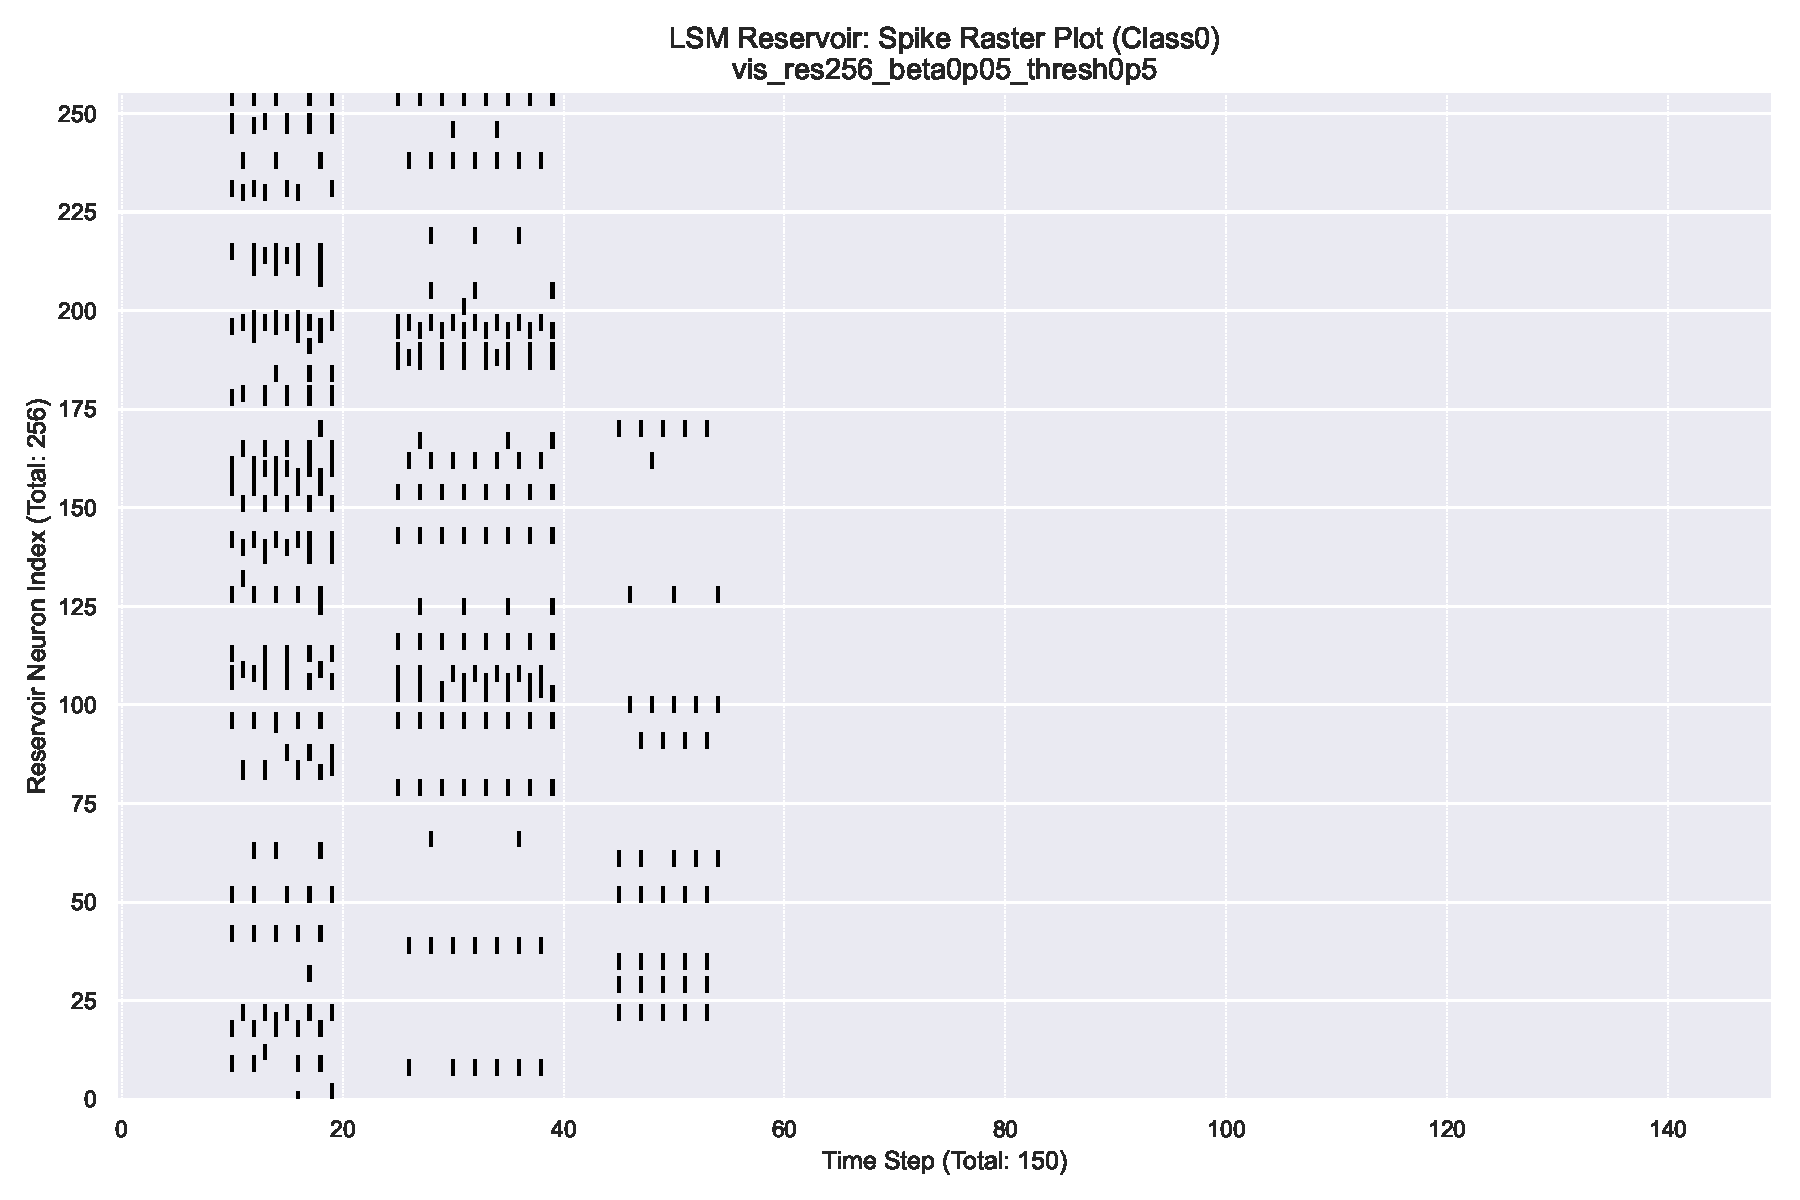
\includegraphics[height=0.55\textheight]{pictures/chLSMEmbeddings/lsm_spike_raster_vis_res256_beta0p05_thresh0p5_Class0.pdf}\\
      \srccap{Reservoir spike raster, $\beta=0.05$, $V_\text{th}=0.5$}
    \end{column}
  \end{columns}
\end{frame}

\begin{frame}{Driven contraction}
  \vspace{0.6em}
  Stability criterion --- maximal conditional Lyapunov exponent:
  \[
    \lambda_1^{(\text{driven})} < 0
  \]
  \vspace{0.6em}
  \begin{alertblock}{Measured on SHAPE ERPs}
    \centering\large $\lambda_1 = -0.054$ \quad\textbar\quad 100\% negative \quad\textbar\quad $N=4{,}220$
  \end{alertblock}
  \vspace{0.4em}
  \begin{center}\small\color{sbnavy}
    Theory predicts contraction. Measurement confirms it.
  \end{center}
\end{frame}

\begin{frame}{The contraction measurement, visualized}
  \begin{columns}[T]
    \begin{column}{0.5\textwidth}\centering
      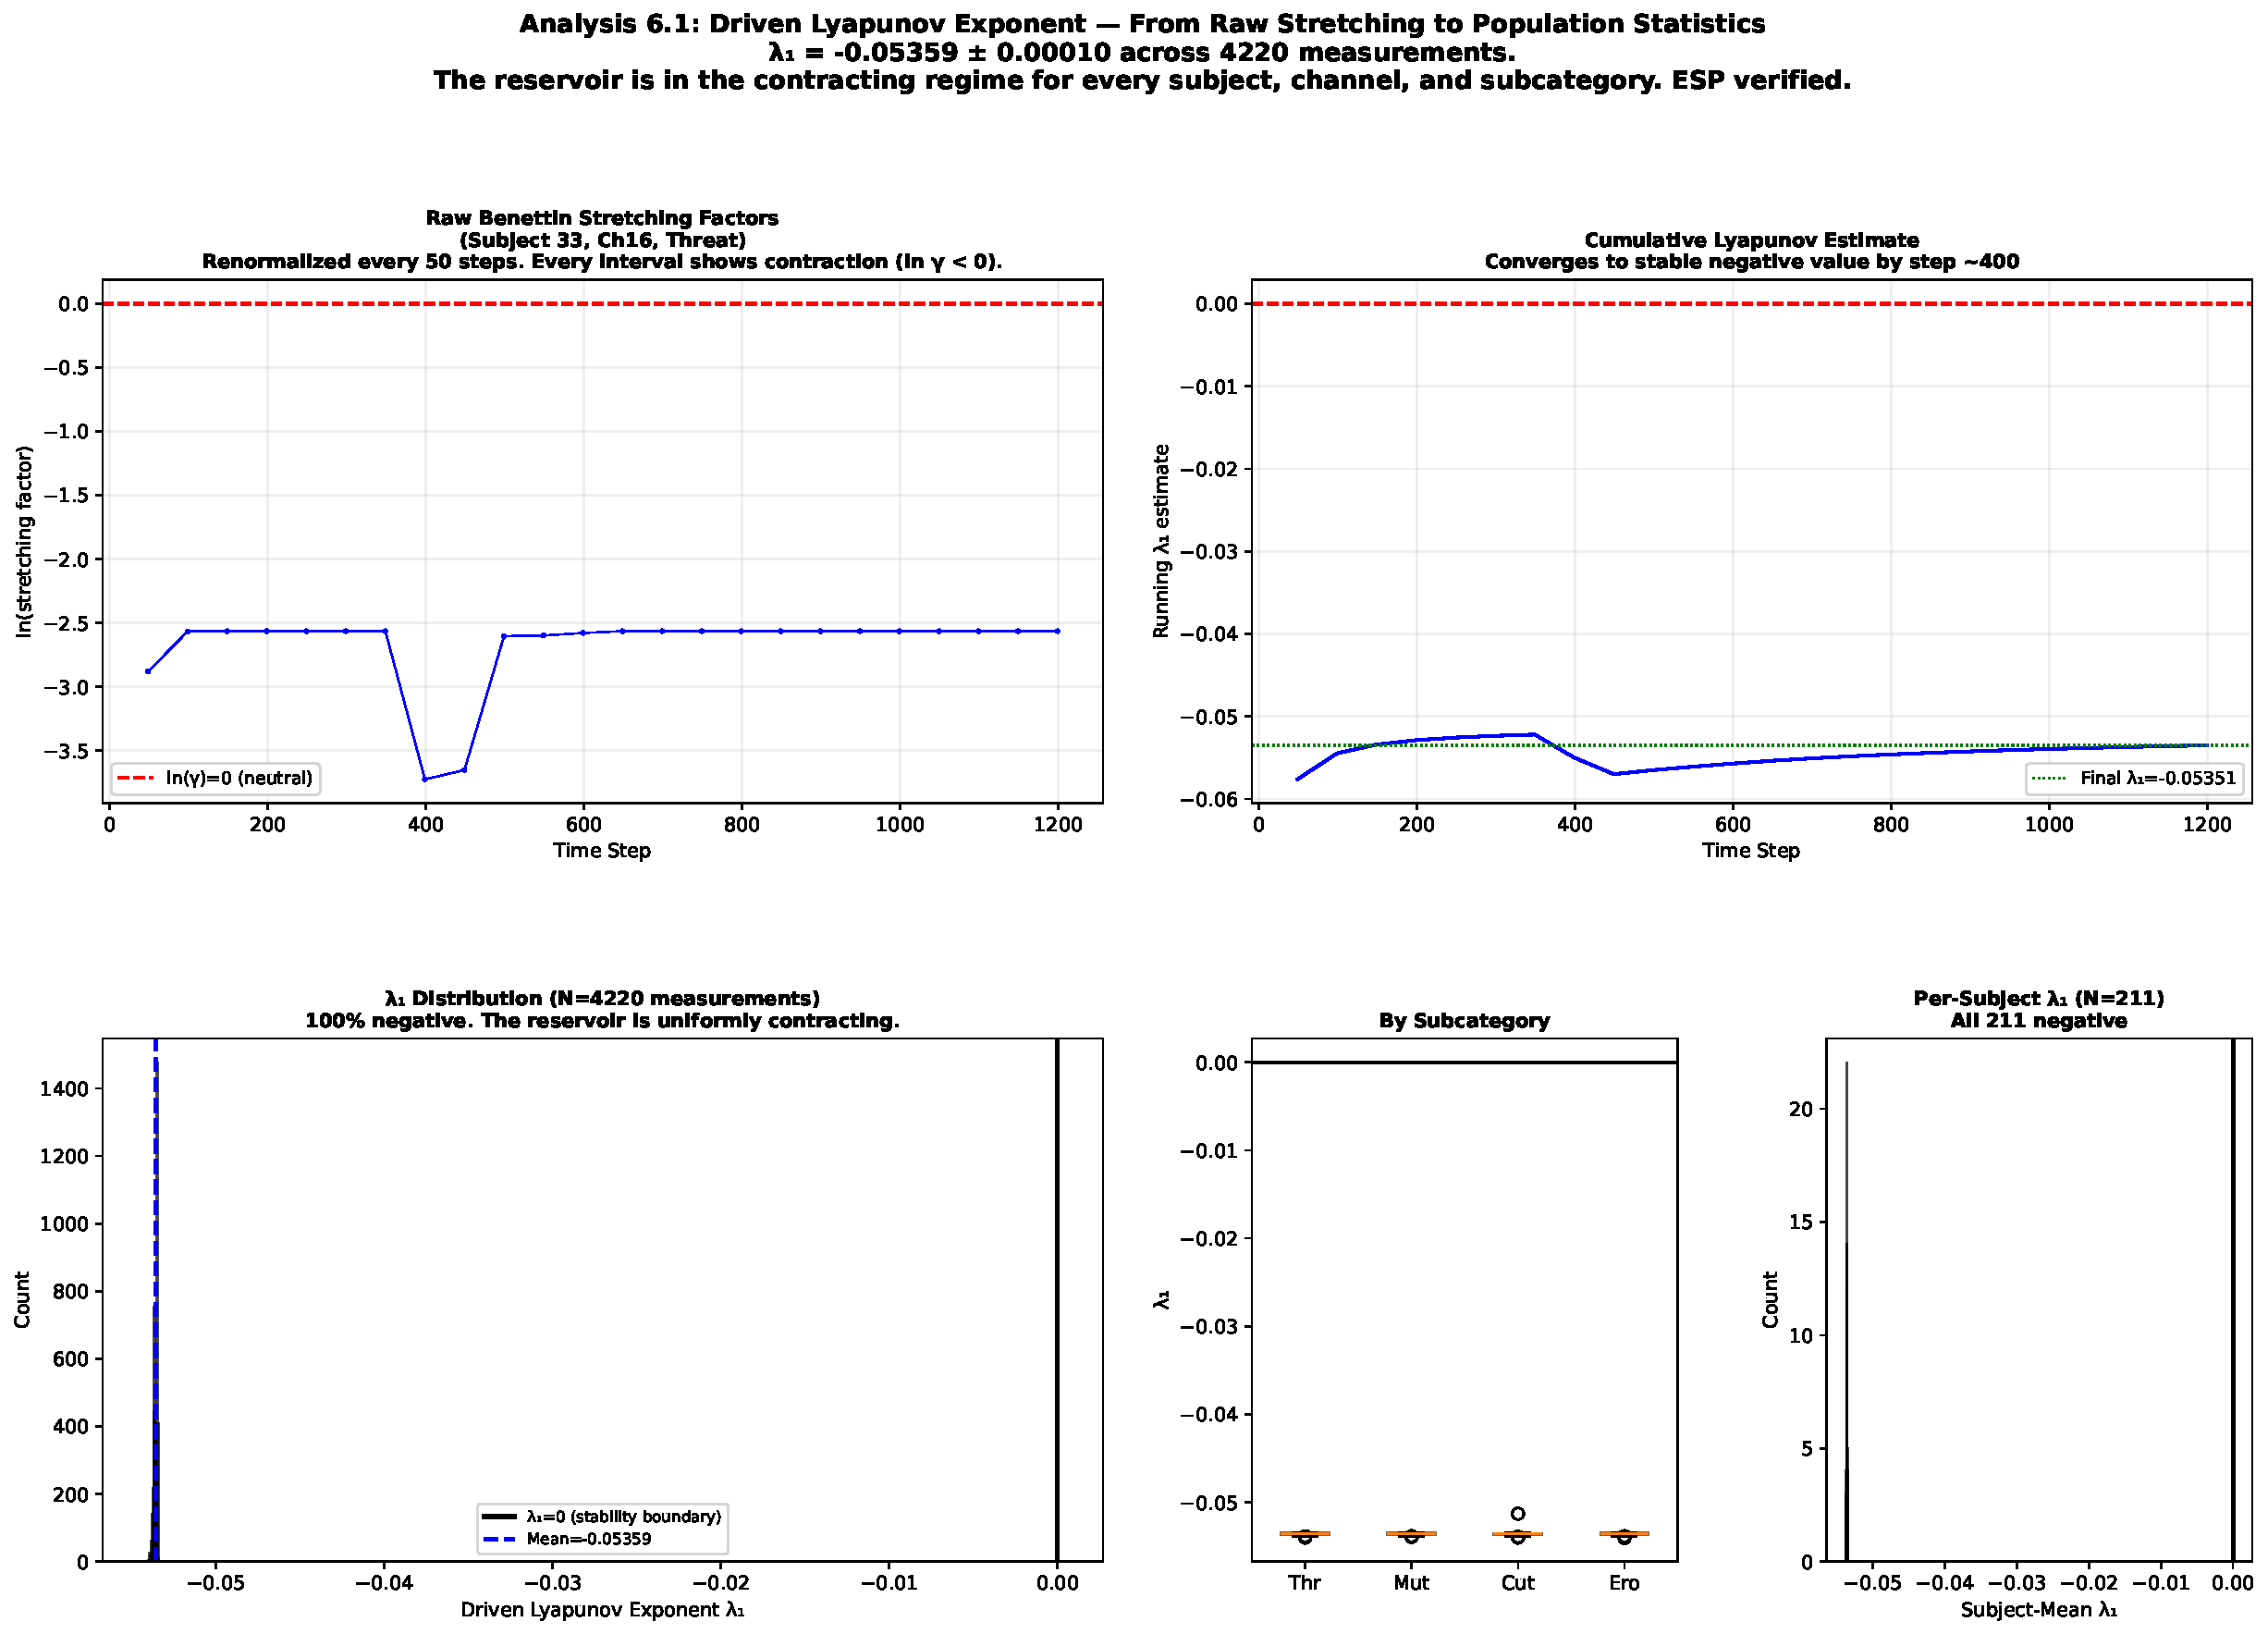
\includegraphics[height=0.55\textheight]{pictures/chDynamics/analysis6_1f_lyapunov.pdf}\\
      \srccap{$\lambda_1$ distribution, $N{=}4220$, $100\%$ negative}
    \end{column}
    \begin{column}{0.5\textwidth}\centering
      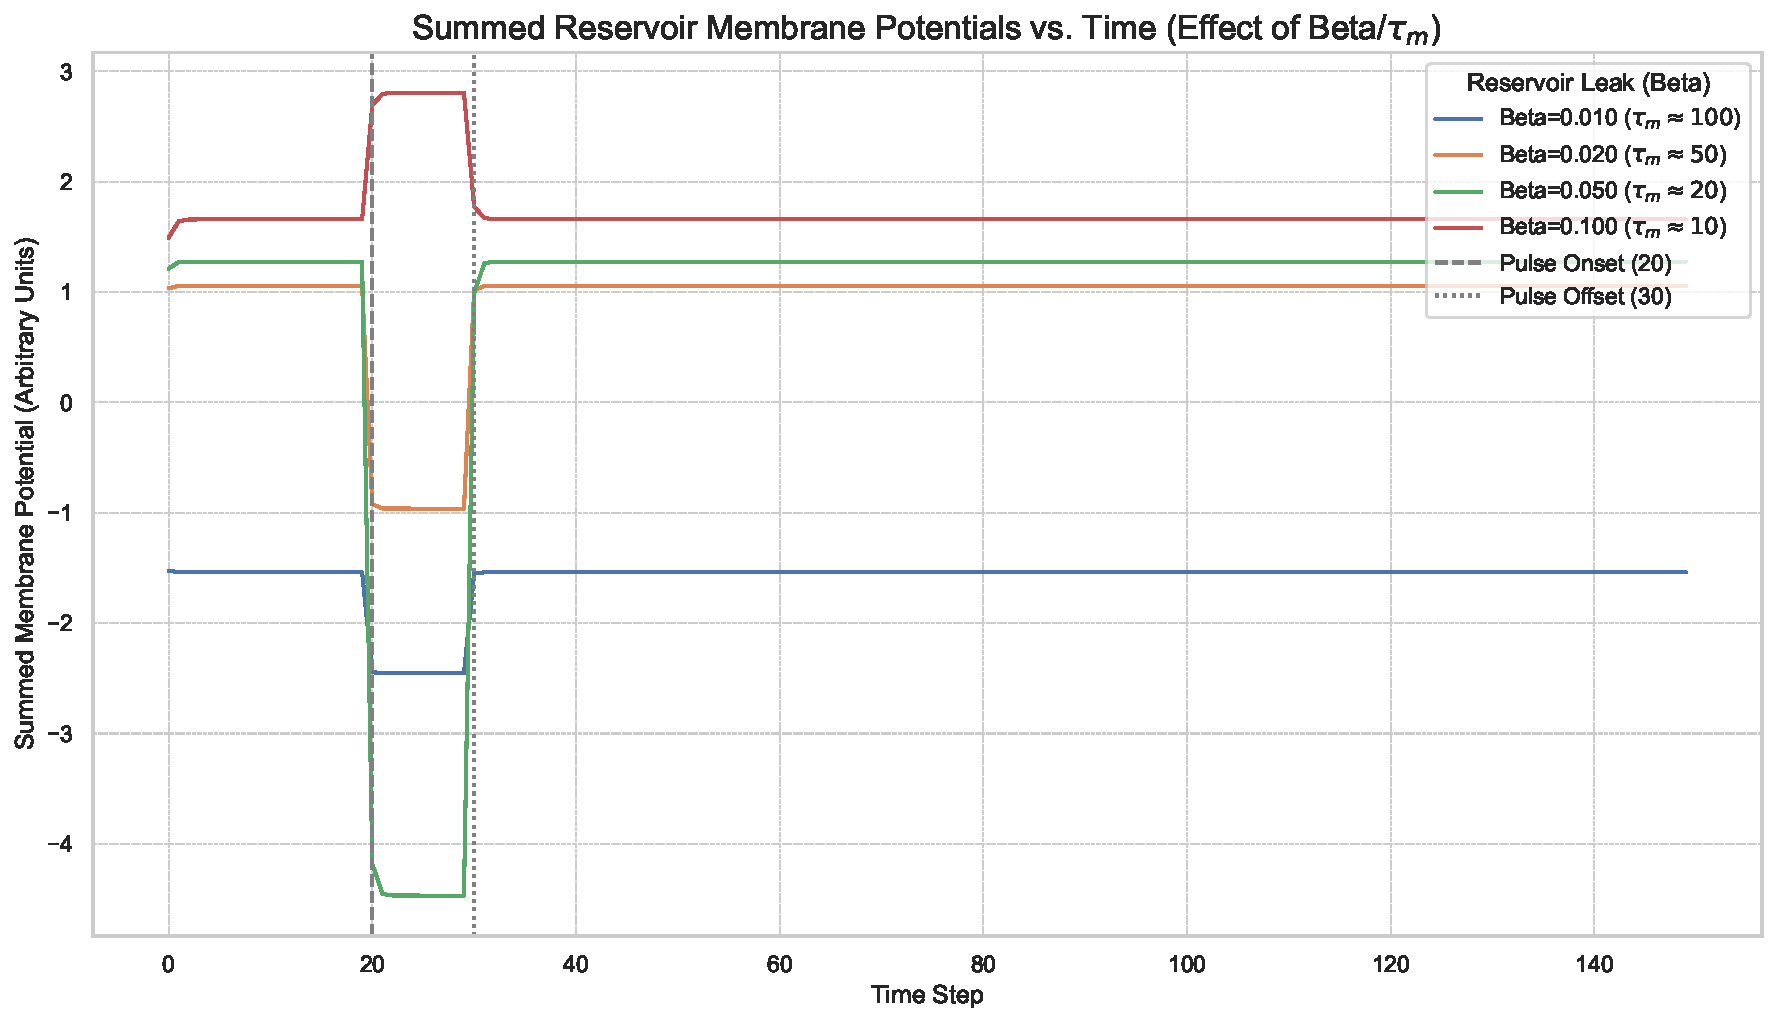
\includegraphics[height=0.55\textheight]{pictures/chLSM/lsm_summed_activity_beta_comparison.pdf}\\
      \srccap{Activity regime across leak $\beta$}
    \end{column}
  \end{columns}
\end{frame}
\begin{frame}{Defense audit: autonomous $\rho(W)$ vs.\ driven $\lambda_1$}
  \begin{columns}[T]
    \begin{column}{0.62\textwidth}
      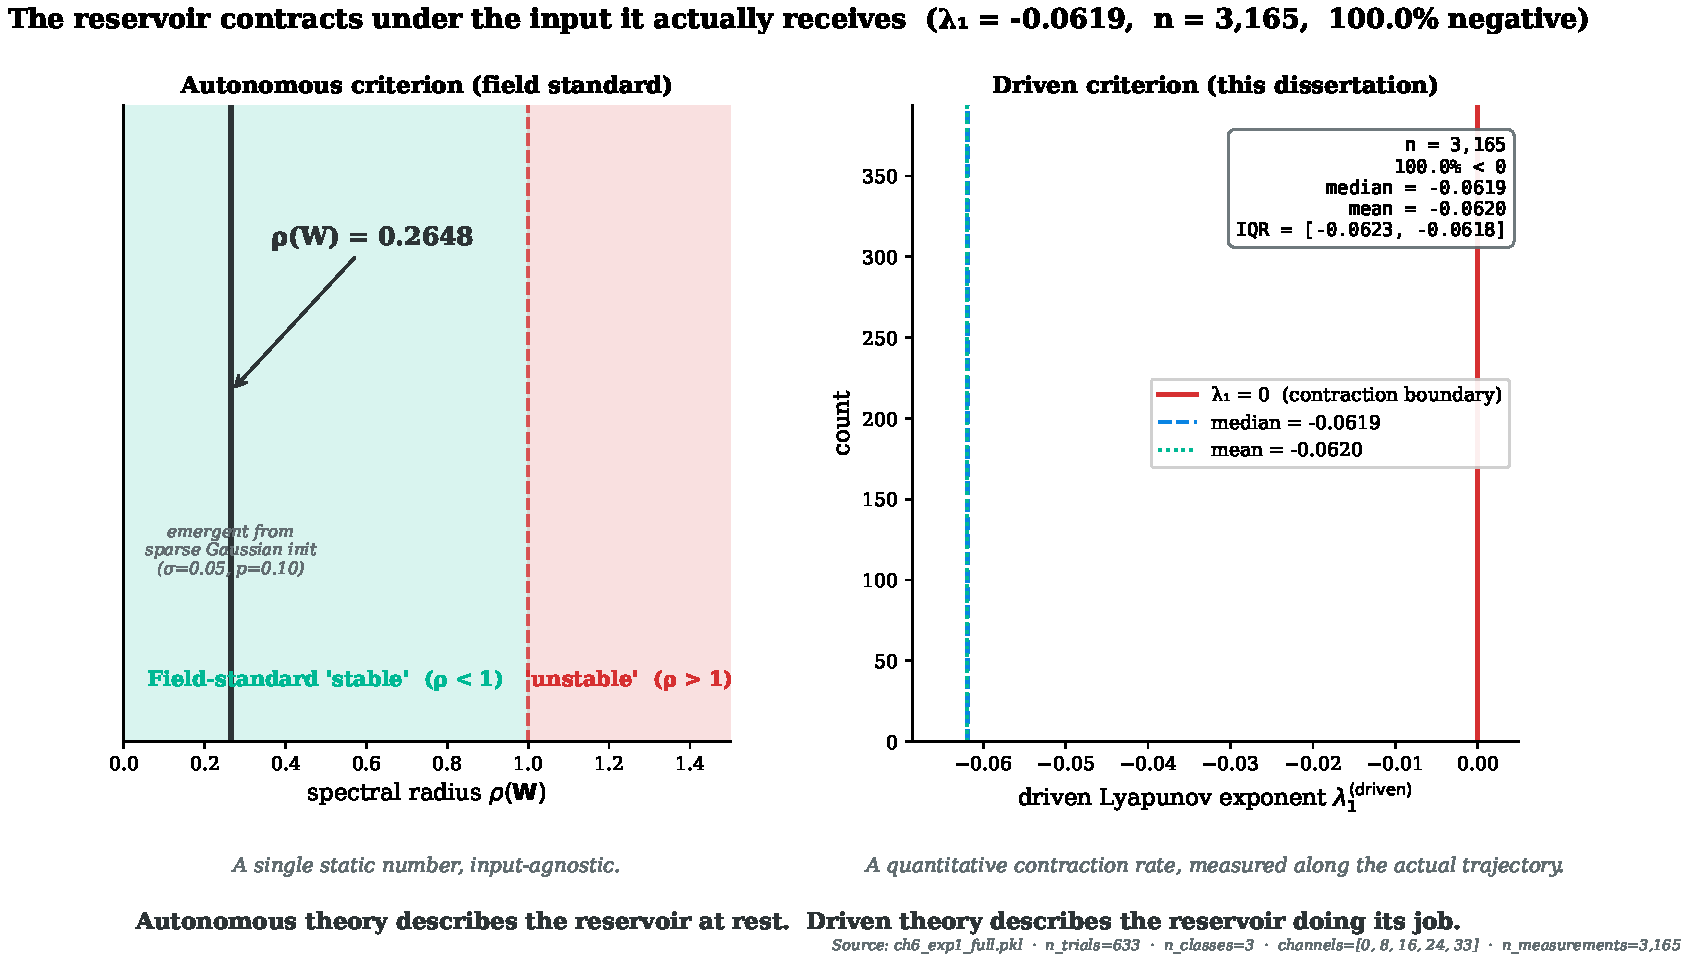
\includegraphics[width=\textwidth]{pictures/defense_audit/analysisA_1e_autonomous_vs_driven.pdf}
    \end{column}
    \begin{column}{0.38\textwidth}\small
      Autonomous spectral radius $\rho(W) = 0.265$ predicts \emph{nothing}
      about driven behavior. Stability is a measured property of the
      reservoir \alert{in operation}, not a cited property of $W$ in
      isolation.
      \vspace{0.4em}
      \begin{itemize}\small
        \item Driven $\lambda_1$ via Benettin on $3{,}165$ real ERP
              trajectories.
        \item Field-default ESN criterion replaced by a measurement.
      \end{itemize}
    \end{column}
  \end{columns}
\end{frame}

\begin{frame}{Temporal coding by design: BSC$_6$}
  Rate coding integrates a spike train to its mean; the temporal structure
  that carries the signal is discarded. We adopt Binned Spike Count with six
  bins:
  \begin{equation*}
    \mathbf{B}_{c,b} = \sum_{t\in W_b} \mathbf{S}^{(c)}(t), \quad b\in\{1,\dots,6\}.
  \end{equation*}
  Six bins align to the canonical ERP windows (N1, P200, P300, LPP) without
  splitting components. This is a principled design choice; a bin-count
  ablation is defined future work.
  \begin{columns}[T]
    \begin{column}{0.55\textwidth}\centering
      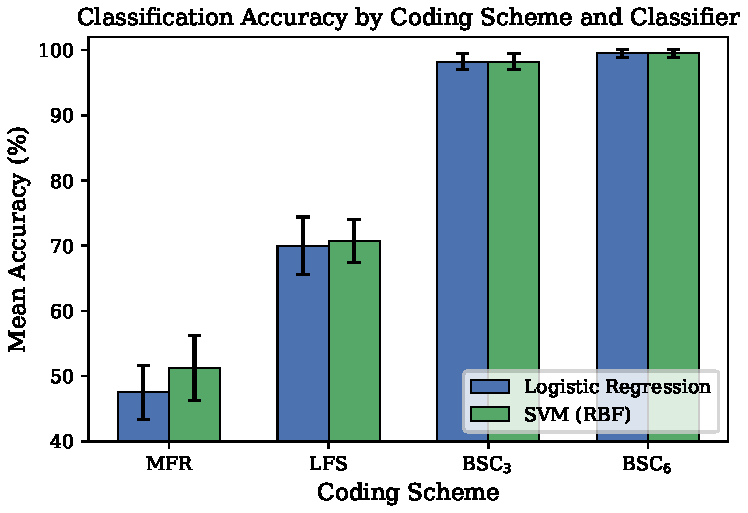
\includegraphics[width=\textwidth]{pictures/chLSMEmbeddings/coding_scheme_accuracy_comparison.pdf}
    \end{column}
    \begin{column}{0.45\textwidth}\small
      The gap from MFR to BSC$_6$ \emph{measures} where the discriminative
      information lives: in the temporal distribution of spikes, not the mean
      rate.
    \end{column}
  \end{columns}
\end{frame}

\begin{frame}{The spike-to-embedding pipeline (Contribution 2)}
  \[
    \underbrace{x_c(t)}_{\text{raw}} \xrightarrow{\text{LIF}} \underbrace{\mathbf{S}_c(t)}_{\text{spikes}} \xrightarrow{\text{BSC}_6} \underbrace{\mathbf{B}_c \in \mathbb{R}^{1536}}_{\text{temporal code}} \xrightarrow{\text{PCA-64}} \underbrace{\mathbf{H}_c \in \mathbb{R}^{64}}_{\text{embedding}}
  \]
  \begin{columns}[T]
    \begin{column}{0.5\textwidth}\centering
      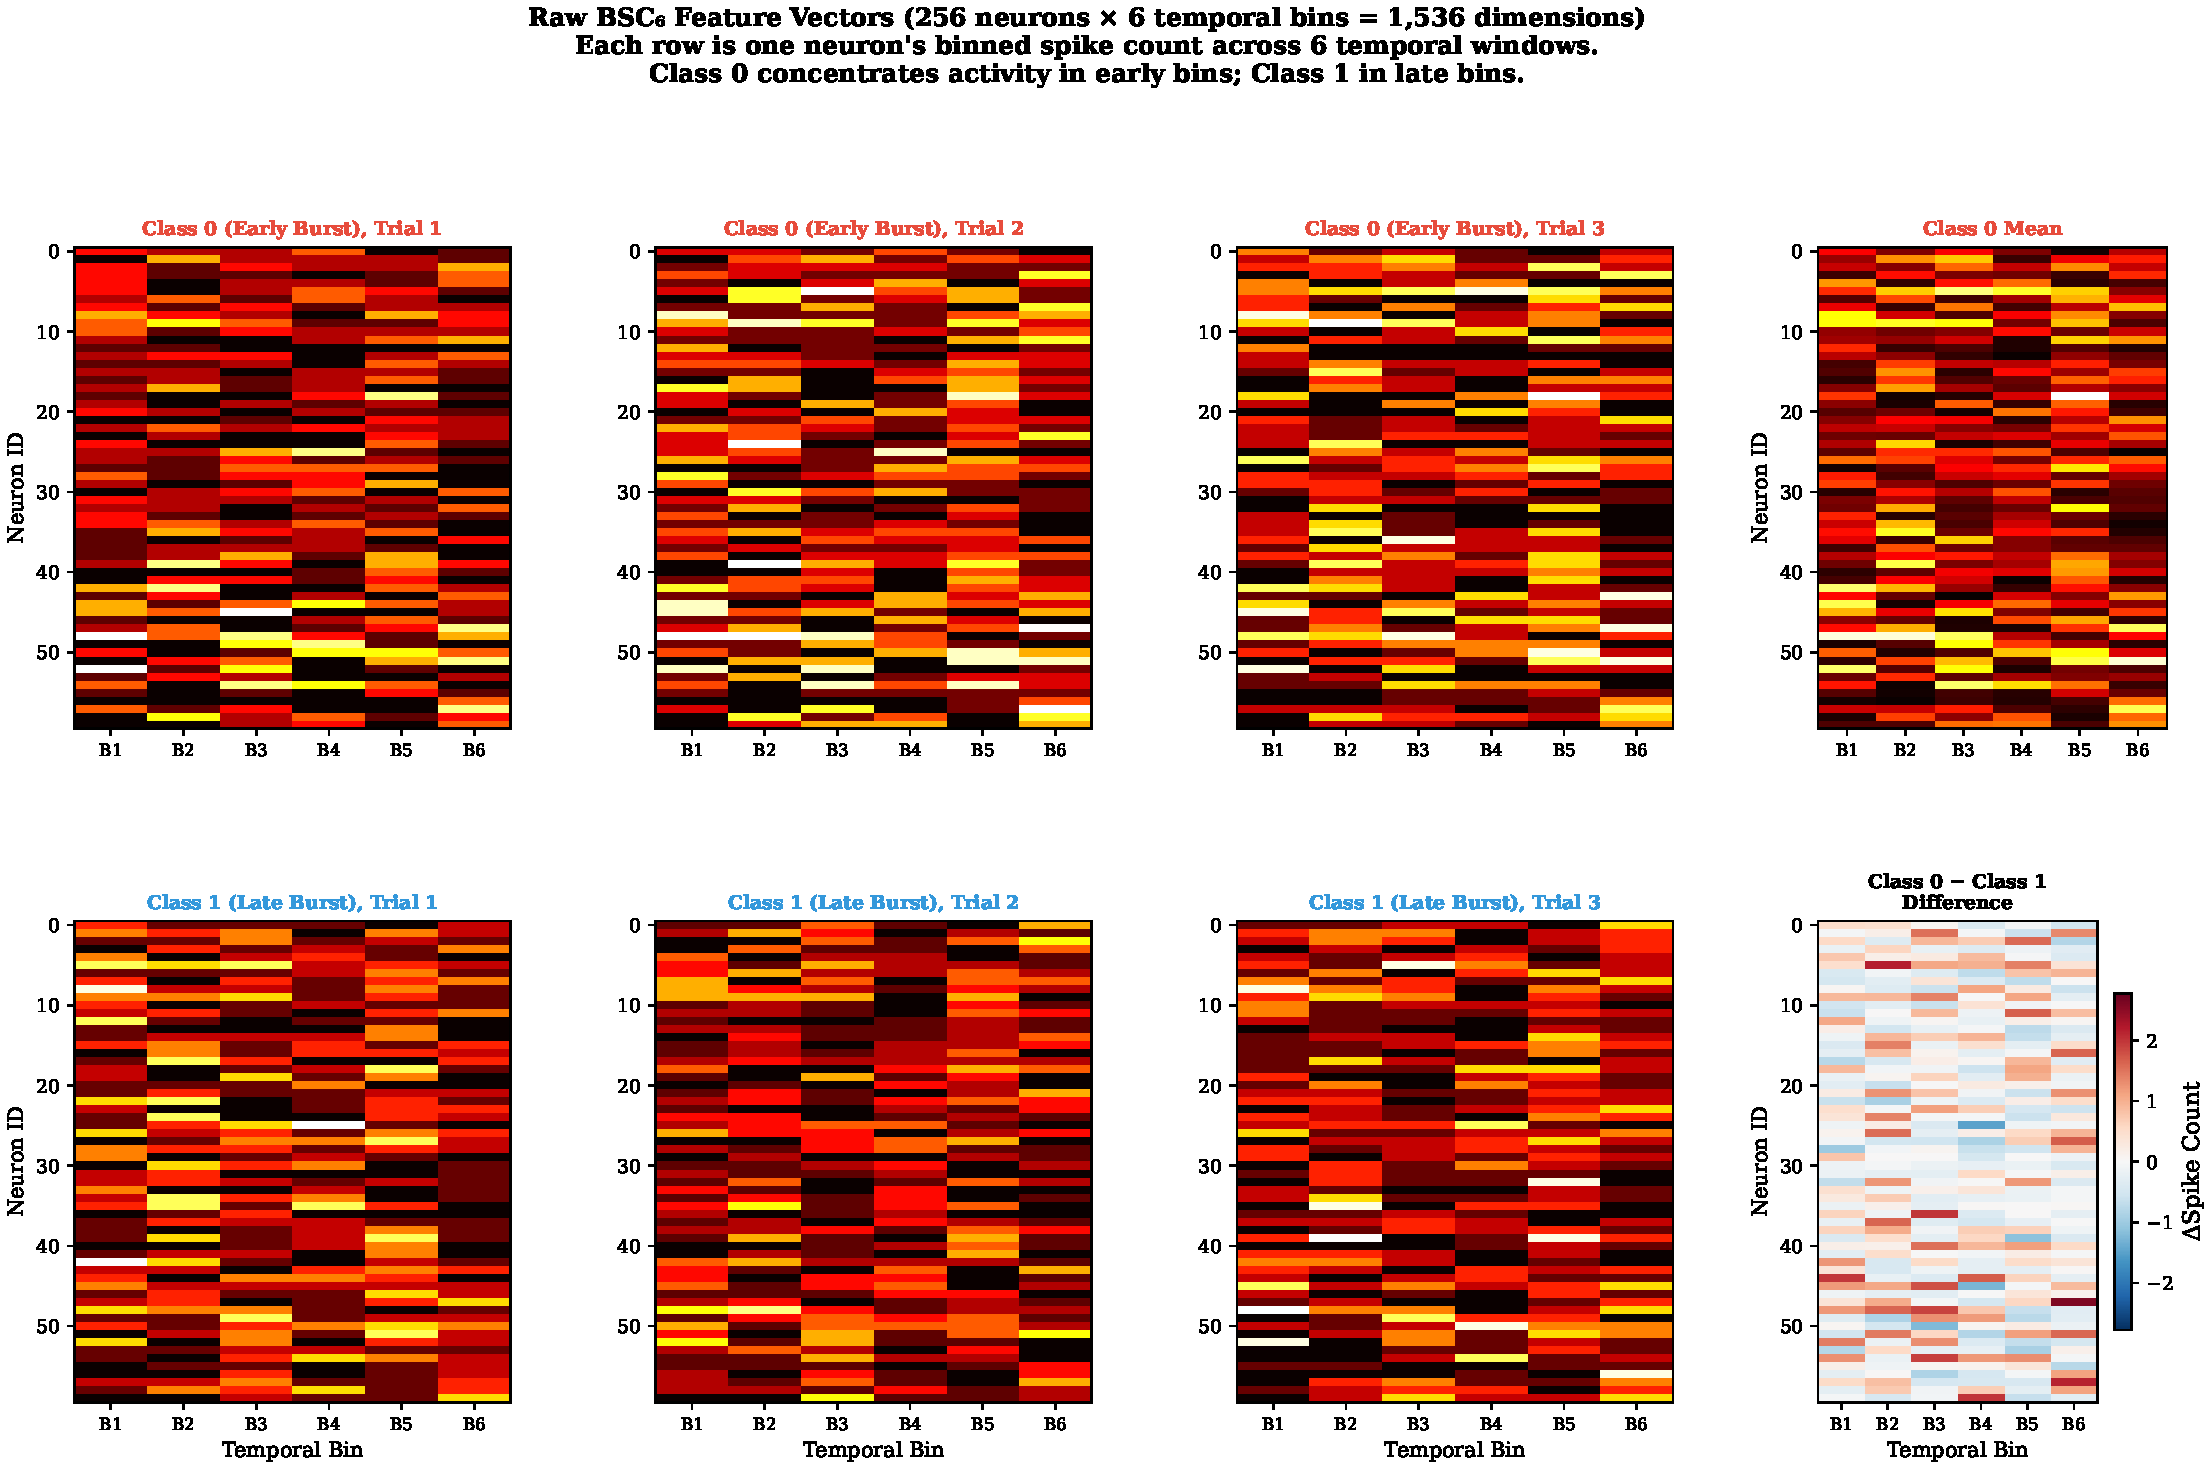
\includegraphics[height=0.4\textheight]{pictures/chLSMEmbeddings/obs03_raw_bsc6_features.pdf}\\
      \srccap{BSC$_6$ temporal-bin features}
    \end{column}
    \begin{column}{0.5\textwidth}\centering
      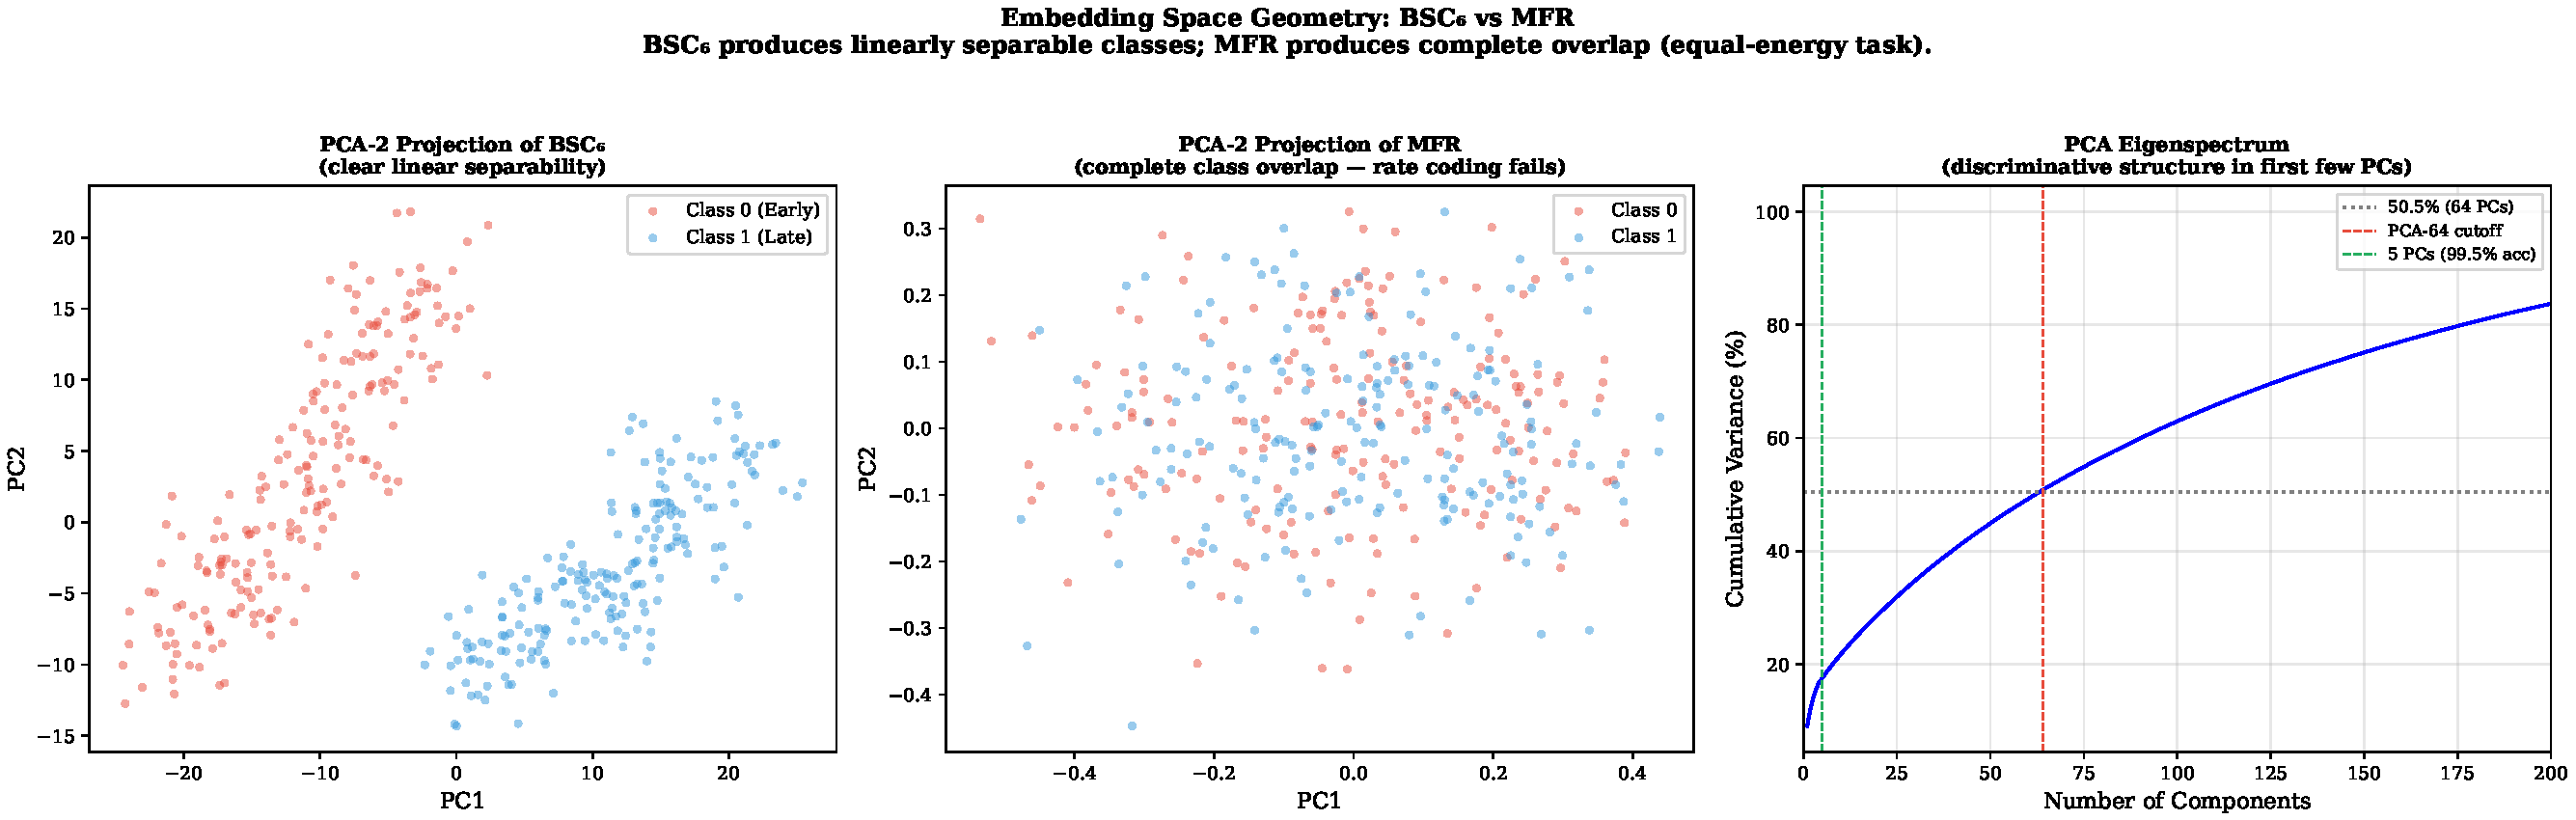
\includegraphics[height=0.4\textheight]{pictures/chLSMEmbeddings/obs04_raw_embedding_space.pdf}\\
      \srccap{PCA-64 embedding geometry}
    \end{column}
  \end{columns}
  \vspace{0.1em}
  {\small Every intermediate is named and traceable. Training-free.
  Initialization-robust ($<2\%$ accuracy variance across reservoir seeds).}
\end{frame}

\begin{frame}{The measurement-instrument paradigm}
  \vspace{0.6em}
  \begin{center}\large
    The reservoir is a \alert{calibrated nonlinear instrument},\\
    not a black-box feature generator.
  \end{center}
  \vspace{0.8em}
  \begin{itemize}
    \item \textbf{Echo-State Property} --- the instrument is reproducible.
    \item \textbf{Data Processing Inequality} --- the reservoir reorganizes
      information; it does not add any.
    \item \textbf{Metric-Specific Validity} --- each descriptor is a named
      physical property of the trajectory.
  \end{itemize}
\end{frame}
\begin{frame}{Defense audit: FNN-measured embedding dimension}
  \begin{columns}[T]
    \begin{column}{0.62\textwidth}
      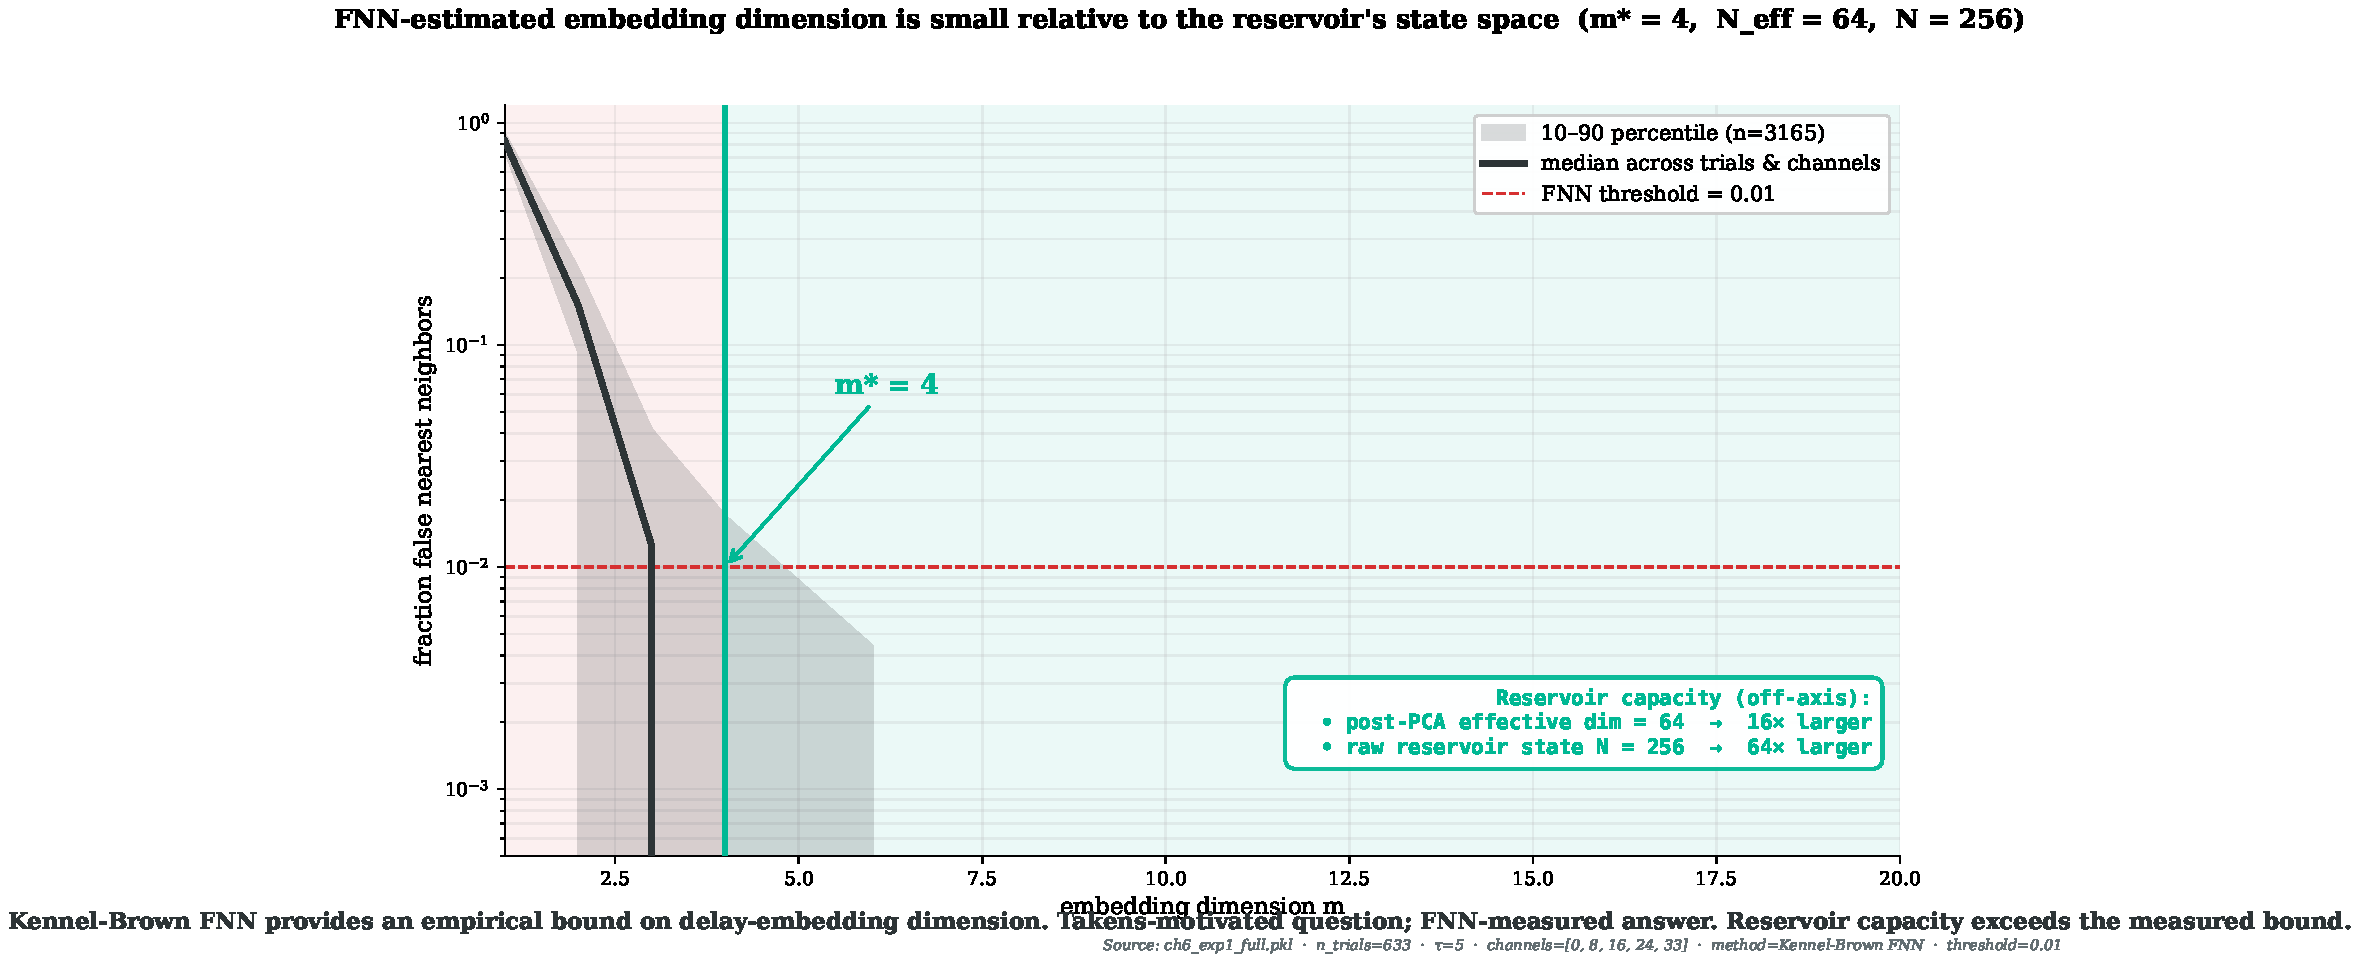
\includegraphics[width=\textwidth]{pictures/defense_audit/analysisB_2e_takens_dimension.pdf}
    \end{column}
    \begin{column}{0.38\textwidth}\small
      Takens motivates the question; Kennel--Brown FNN supplies the
      \alert{measurement}. The figure does not claim Takens
      ``guarantees'' attractor reconstruction.
      \vspace{0.4em}
      \begin{itemize}\small
        \item Measured $m^{*} \ll 64$ (post-PCA) $\ll 256$ (raw).
        \item Reservoir state capacity comfortably exceeds the bound.
      \end{itemize}
    \end{column}
  \end{columns}
\end{frame}

\begin{frame}{The path to silicon}
  \vspace{0.6em}
  Energy is motivational here, not measured.
  \vspace{0.8em}
  \begin{itemize}
    \item RSNN on Loihi: $\sim$$983\times$ vs.\ GPU.
    \item Activity SNN on Loihi: $2\times$ EDP at matched accuracy.
    \item NeuCube on SpiNNaker --- portable, low-power.
  \end{itemize}
  \vspace{0.8em}
  \begin{center}\color{sbnavy}
    Loihi 2 / LAVA is the defined next measurement.
  \end{center}
\end{frame}

\begin{frame}{The failure of spatial deep learning}
  \vspace{0.8em}
  \begin{itemize}
    \item \textbf{Hypothesis:} GAT captures inter-electrode connectivity.
    \item \alert{Hypothesis failed.} Message-passing over-smoothed the
      spike-domain features.
    \item Not a hyperparameter problem --- a theoretical mismatch.
    \item Pivot: graph-topological descriptors.
  \end{itemize}
  \vspace{0.8em}
  \begin{center}
    \small\color{sbnavy} The pivot was possible because the pipeline was
    transparent enough to diagnose the failure mechanism.
  \end{center}
\end{frame}

% ===============================================================
\section{Part 4 --- The Three Operationally Distinct Layers}
% ===============================================================

\begin{frame}{The three-layer structure}
  \vspace{0.6em}
  \begin{center}\large
    Three layers $\cdot$ Three measurements $\cdot$ Three properties
  \end{center}
  \vspace{1.0em}
  \begin{itemize}
    \item \textbf{A. Discriminative Embedding} --- the condition signal.
    \item \textbf{B. Dynamical Response} --- trajectory characterization.
    \item \textbf{C. Topology and Coupling} --- inter-channel organization.
  \end{itemize}
\end{frame}

\begin{frame}{Layer A --- the subject-covariance hinge}
  Raw embedding geometry is dominated by subject identity, not condition.
  Variance decomposition makes this explicit:
  \begin{columns}[T]
    \begin{column}{0.55\textwidth}\centering
      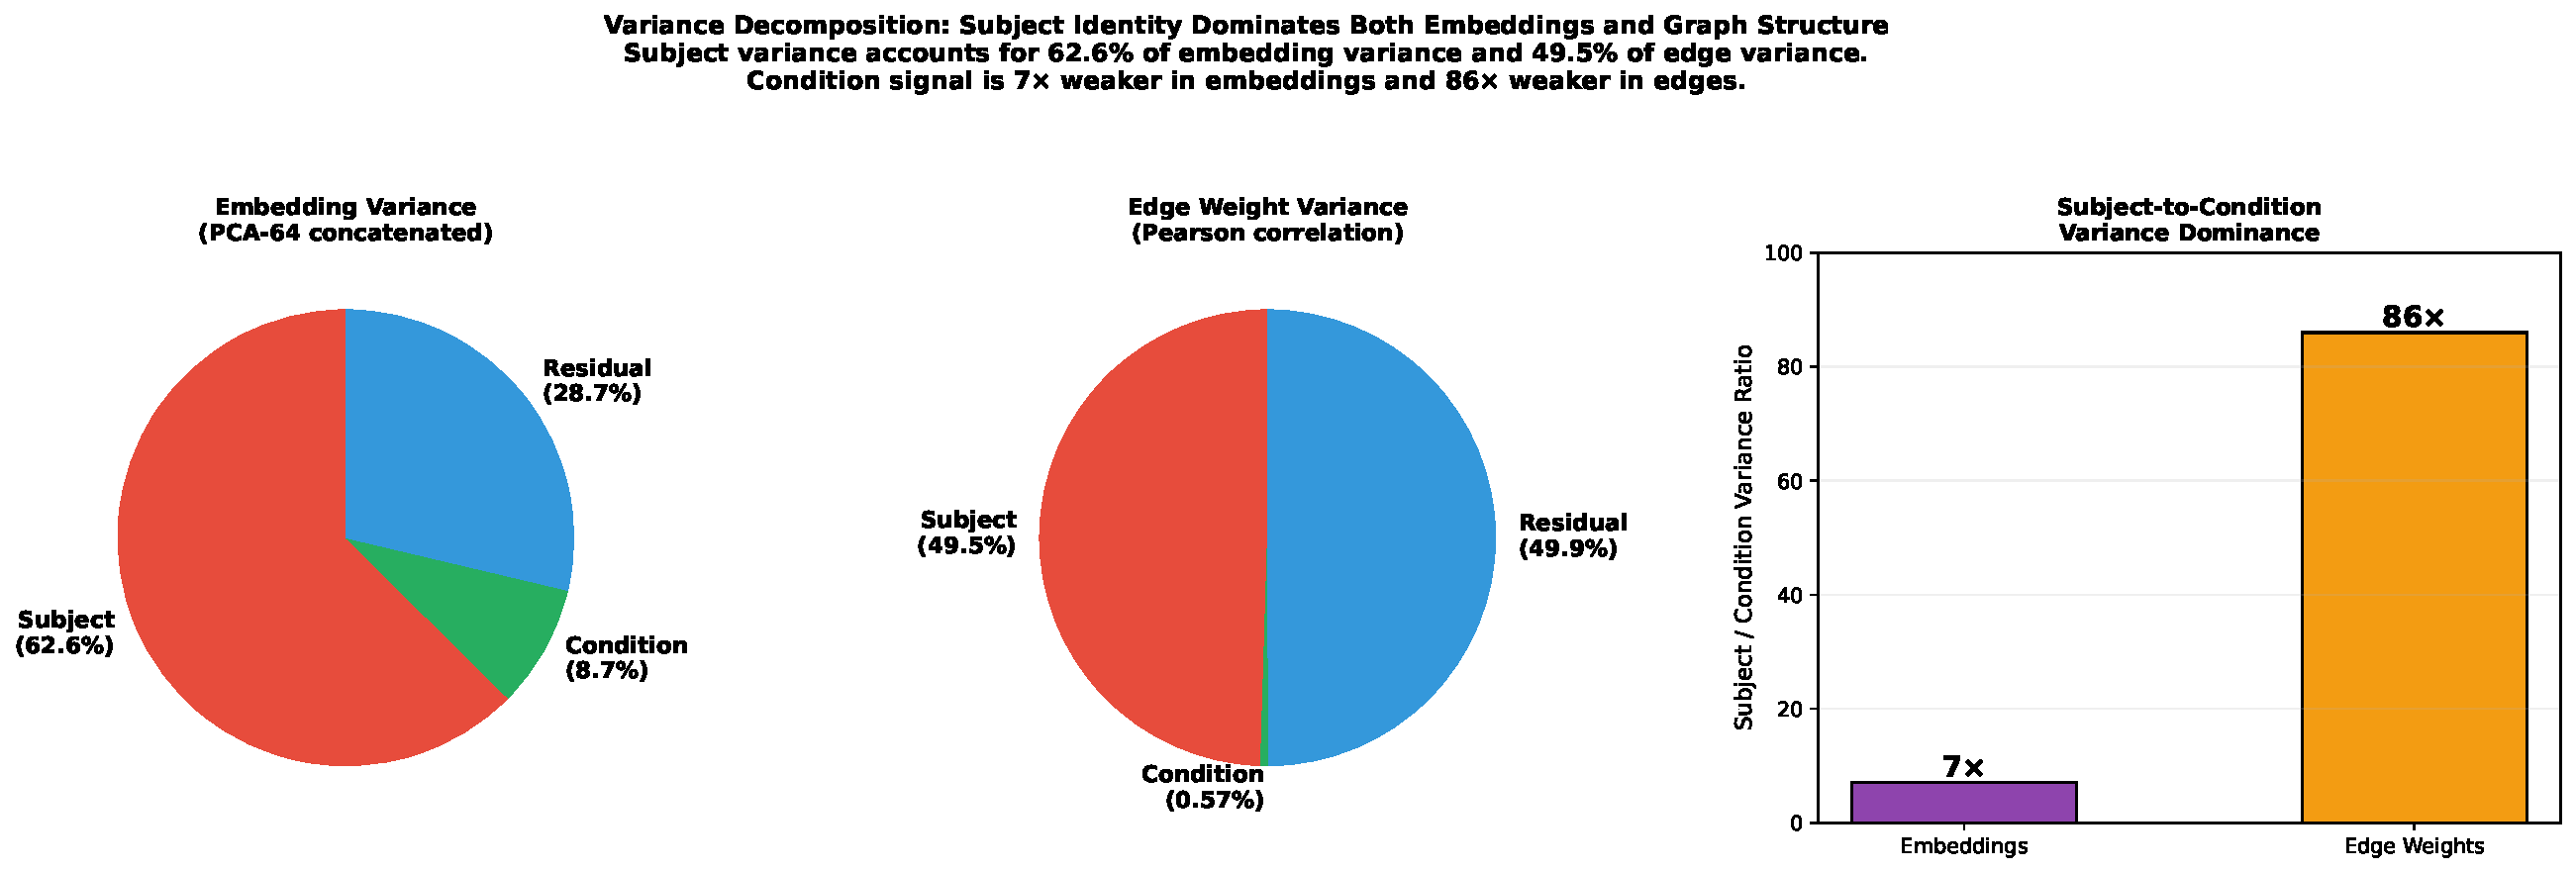
\includegraphics[width=\textwidth]{pictures/chGraphNeuralNetworks/exp01_variance_decomposition.pdf}\\
      \srccap{Variance decomposition: subject vs.\ condition}
    \end{column}
    \begin{column}{0.45\textwidth}\small
      \[
        \rho = \frac{\sigma^2_\text{subject}}{\sigma^2_\text{condition}} = 7.2
      \]
      Per-subject centering
      $\tilde{\mathbf{H}}_p = \mathbf{H}_p - \bar{\mathbf{H}}_p$
      removes the subject-mean offset and exposes the condition order.
      Centering is label-free; the operation estimates within-subject
      separability.
    \end{column}
  \end{columns}
\end{frame}

\begin{frame}{Layer A --- centering is the dominant intervention (Contribution 5)}
  \begin{columns}[T]
    \begin{column}{0.55\textwidth}\centering
      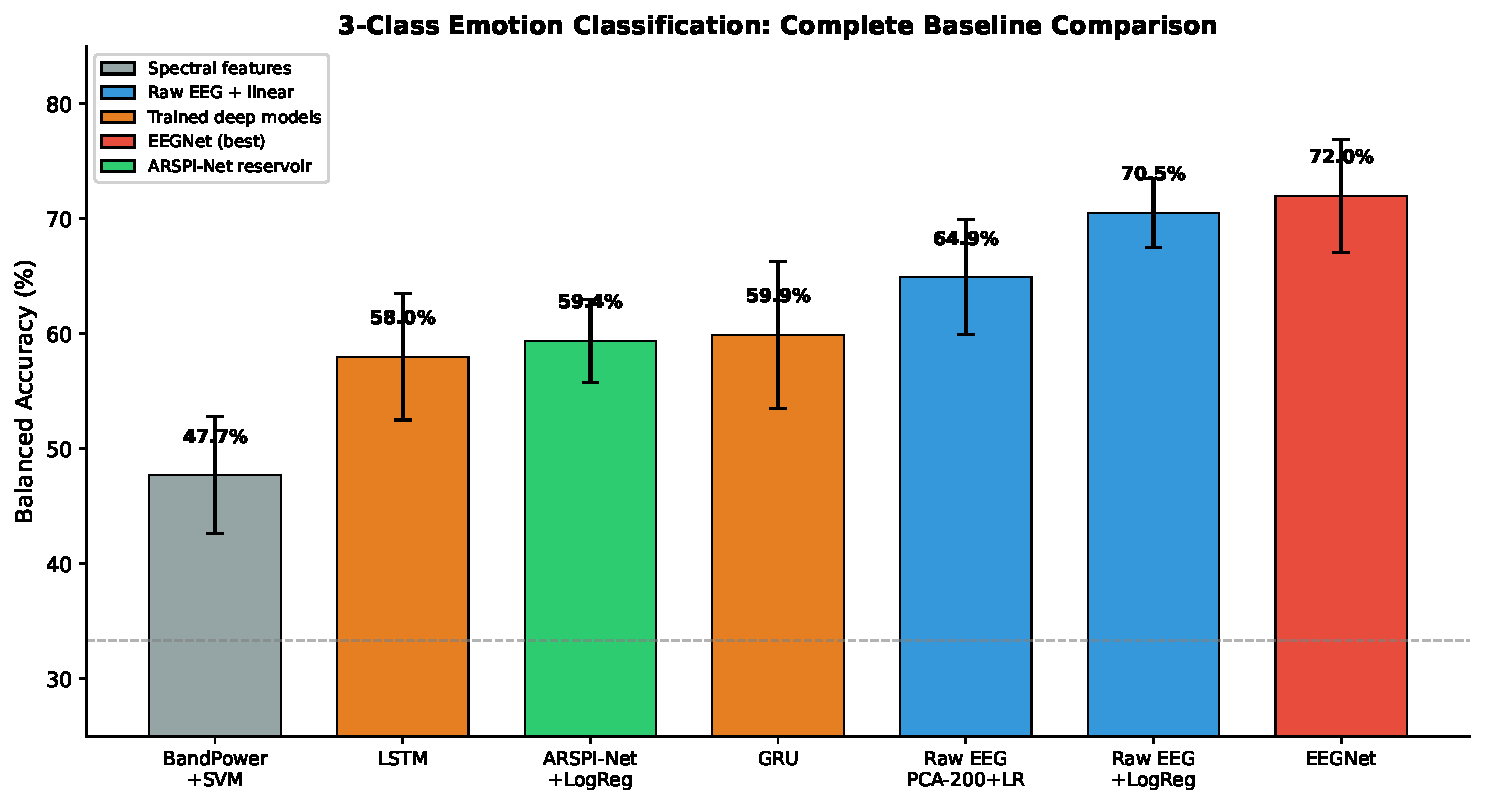
\includegraphics[width=\textwidth]{pictures/chGraphNeuralNetworks/fig_baseline_comparison.pdf}
    \end{column}
    \begin{column}{0.45\textwidth}\small
      \begin{tabular}{lcc}\toprule
        & Uncent.\ & Cent.\ \\\midrule
        EEGNet & 72.0 & 89.1 \\
        Raw EEG & 70.5 & 88.4 \\
        PCA-200 & 64.9 & 86.4 \\
        GRU & 59.9 & 78.4 \\
        \alert{ARSPI-Net} & \alert{59.4} & \alert{78.8} \\
        LSTM & 58.0 & 71.1 \\
        BandPower & 47.7 & 61.0 \\
        \bottomrule
      \end{tabular}
      \vspace{0.3em}

      Centering moves every model $+13$ to $+22$\,pp. After centering,
      ARSPI-Net matches GRU with zero trainable recurrent parameters.
    \end{column}
  \end{columns}
\end{frame}

\begin{frame}{Layer B --- seven named observables}
  \vspace{1.2em}
  \begin{center}
    \textbf{Amplitude family}\\
    total spikes \,$\cdot$\, firing rate \,$\cdot$\, rate variance\\[1em]
    \textbf{Temporal family}\\
    rate entropy \,$\cdot$\, temporal sparsity \,$\cdot$\, $\hat{H}_\pi$ \,$\cdot$\, $\tau_{AC}$
  \end{center}
  \vspace{0.8em}
  \begin{center}\color{sbnavy}\small
    Observables --- not learned features.
  \end{center}
\end{frame}

\begin{frame}{Layer B --- descriptors are condition-sensitive}
  \begin{columns}[T]
    \begin{column}{0.55\textwidth}\centering
      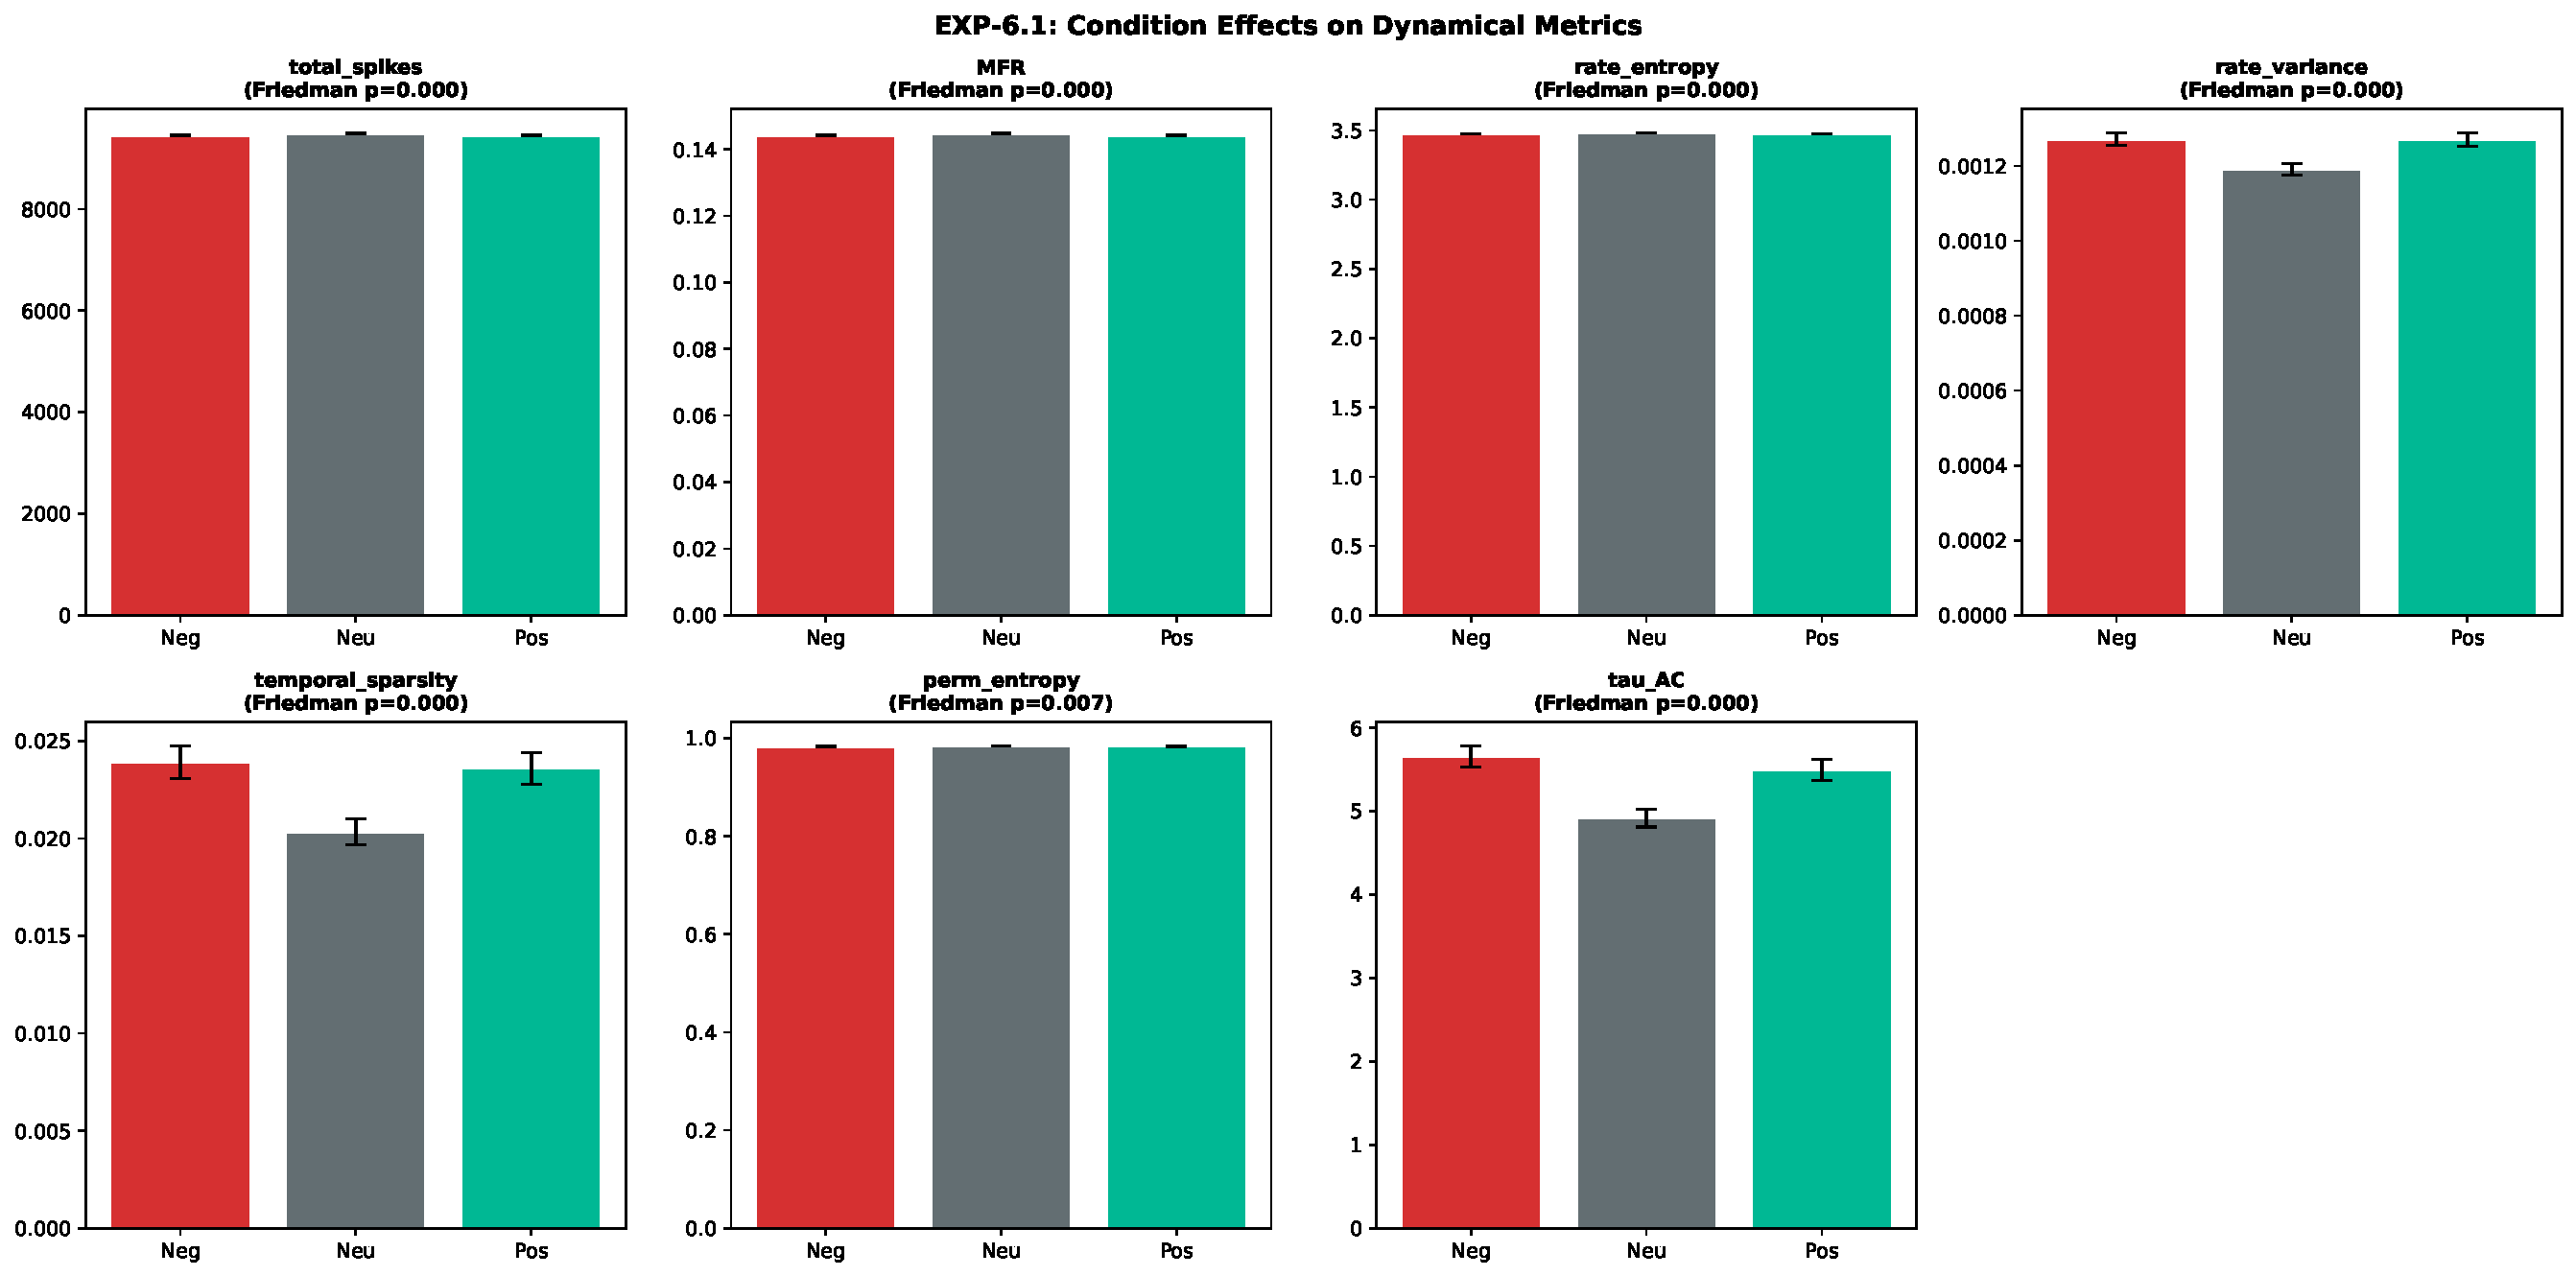
\includegraphics[width=\textwidth]{pictures/chDynamics/fig01_condition_effects.pdf}
    \end{column}
    \begin{column}{0.45\textwidth}\small
      Subject-level Friedman tests: $7/7$ descriptors distinguish emotional
      from non-emotional input ($p<0.05$).
      \vspace{0.3em}

      \alert{Subject-level inference} throughout --- no pseudo-replication
      across observations.
    \end{column}
  \end{columns}
\end{frame}

\begin{frame}{Layer B --- the temporal family dominates}
  \begin{columns}[T]
    \begin{column}{0.55\textwidth}\centering
      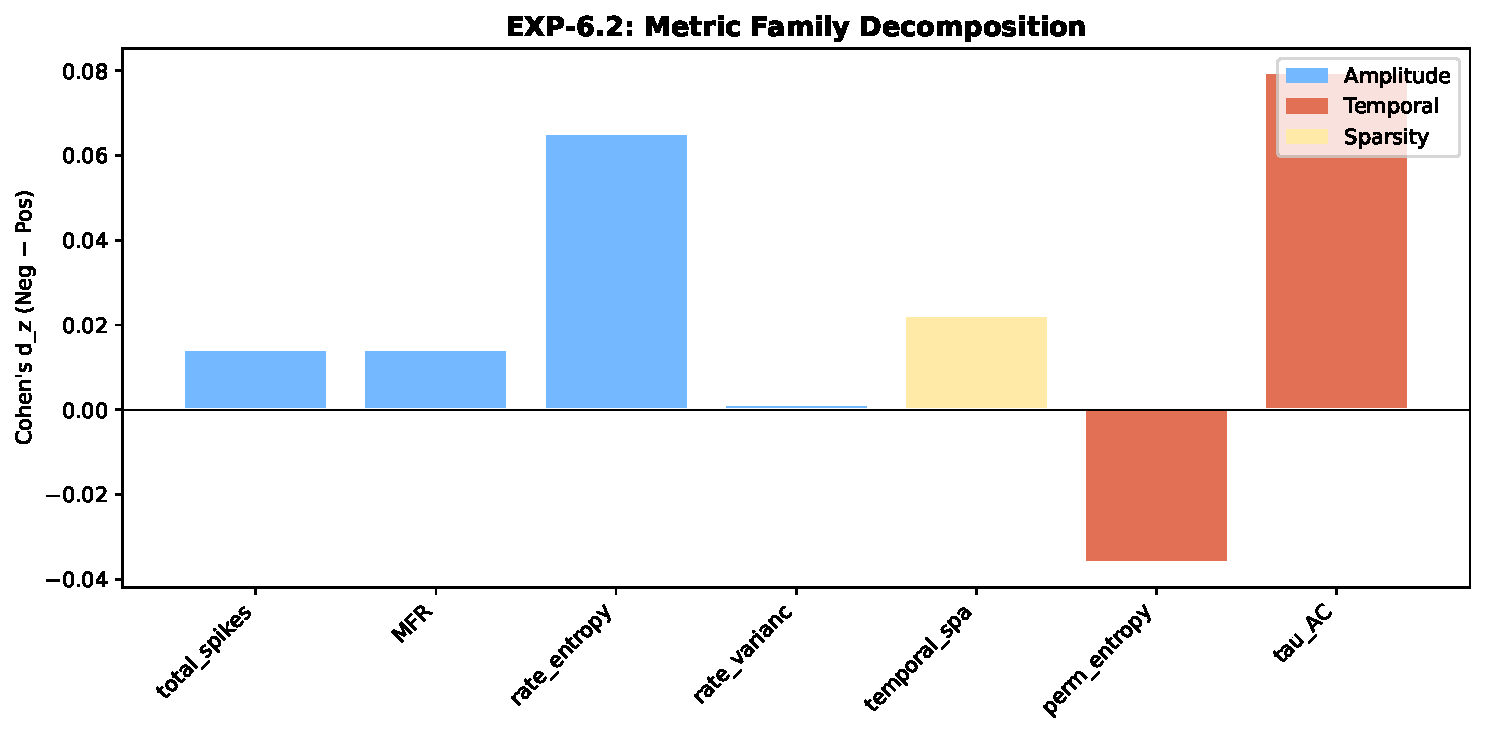
\includegraphics[width=\textwidth]{pictures/chDynamics/fig02_metric_families.pdf}
    \end{column}
    \begin{column}{0.45\textwidth}\small
      The temporal-structure family ($\hat{H}_\pi$, $\tau_{AC}$) carries
      \alert{$2.4\times$ larger} condition effects than the amplitude-tracking
      family.
      \vspace{0.3em}

      An independent confirmation of the temporal-coding premise --- now at
      the level of reservoir dynamics, not just the coding scheme.
    \end{column}
  \end{columns}
\end{frame}

\begin{frame}{Layer B --- the excitability--persistence axis}
  \begin{columns}[T]
    \begin{column}{0.55\textwidth}\centering
      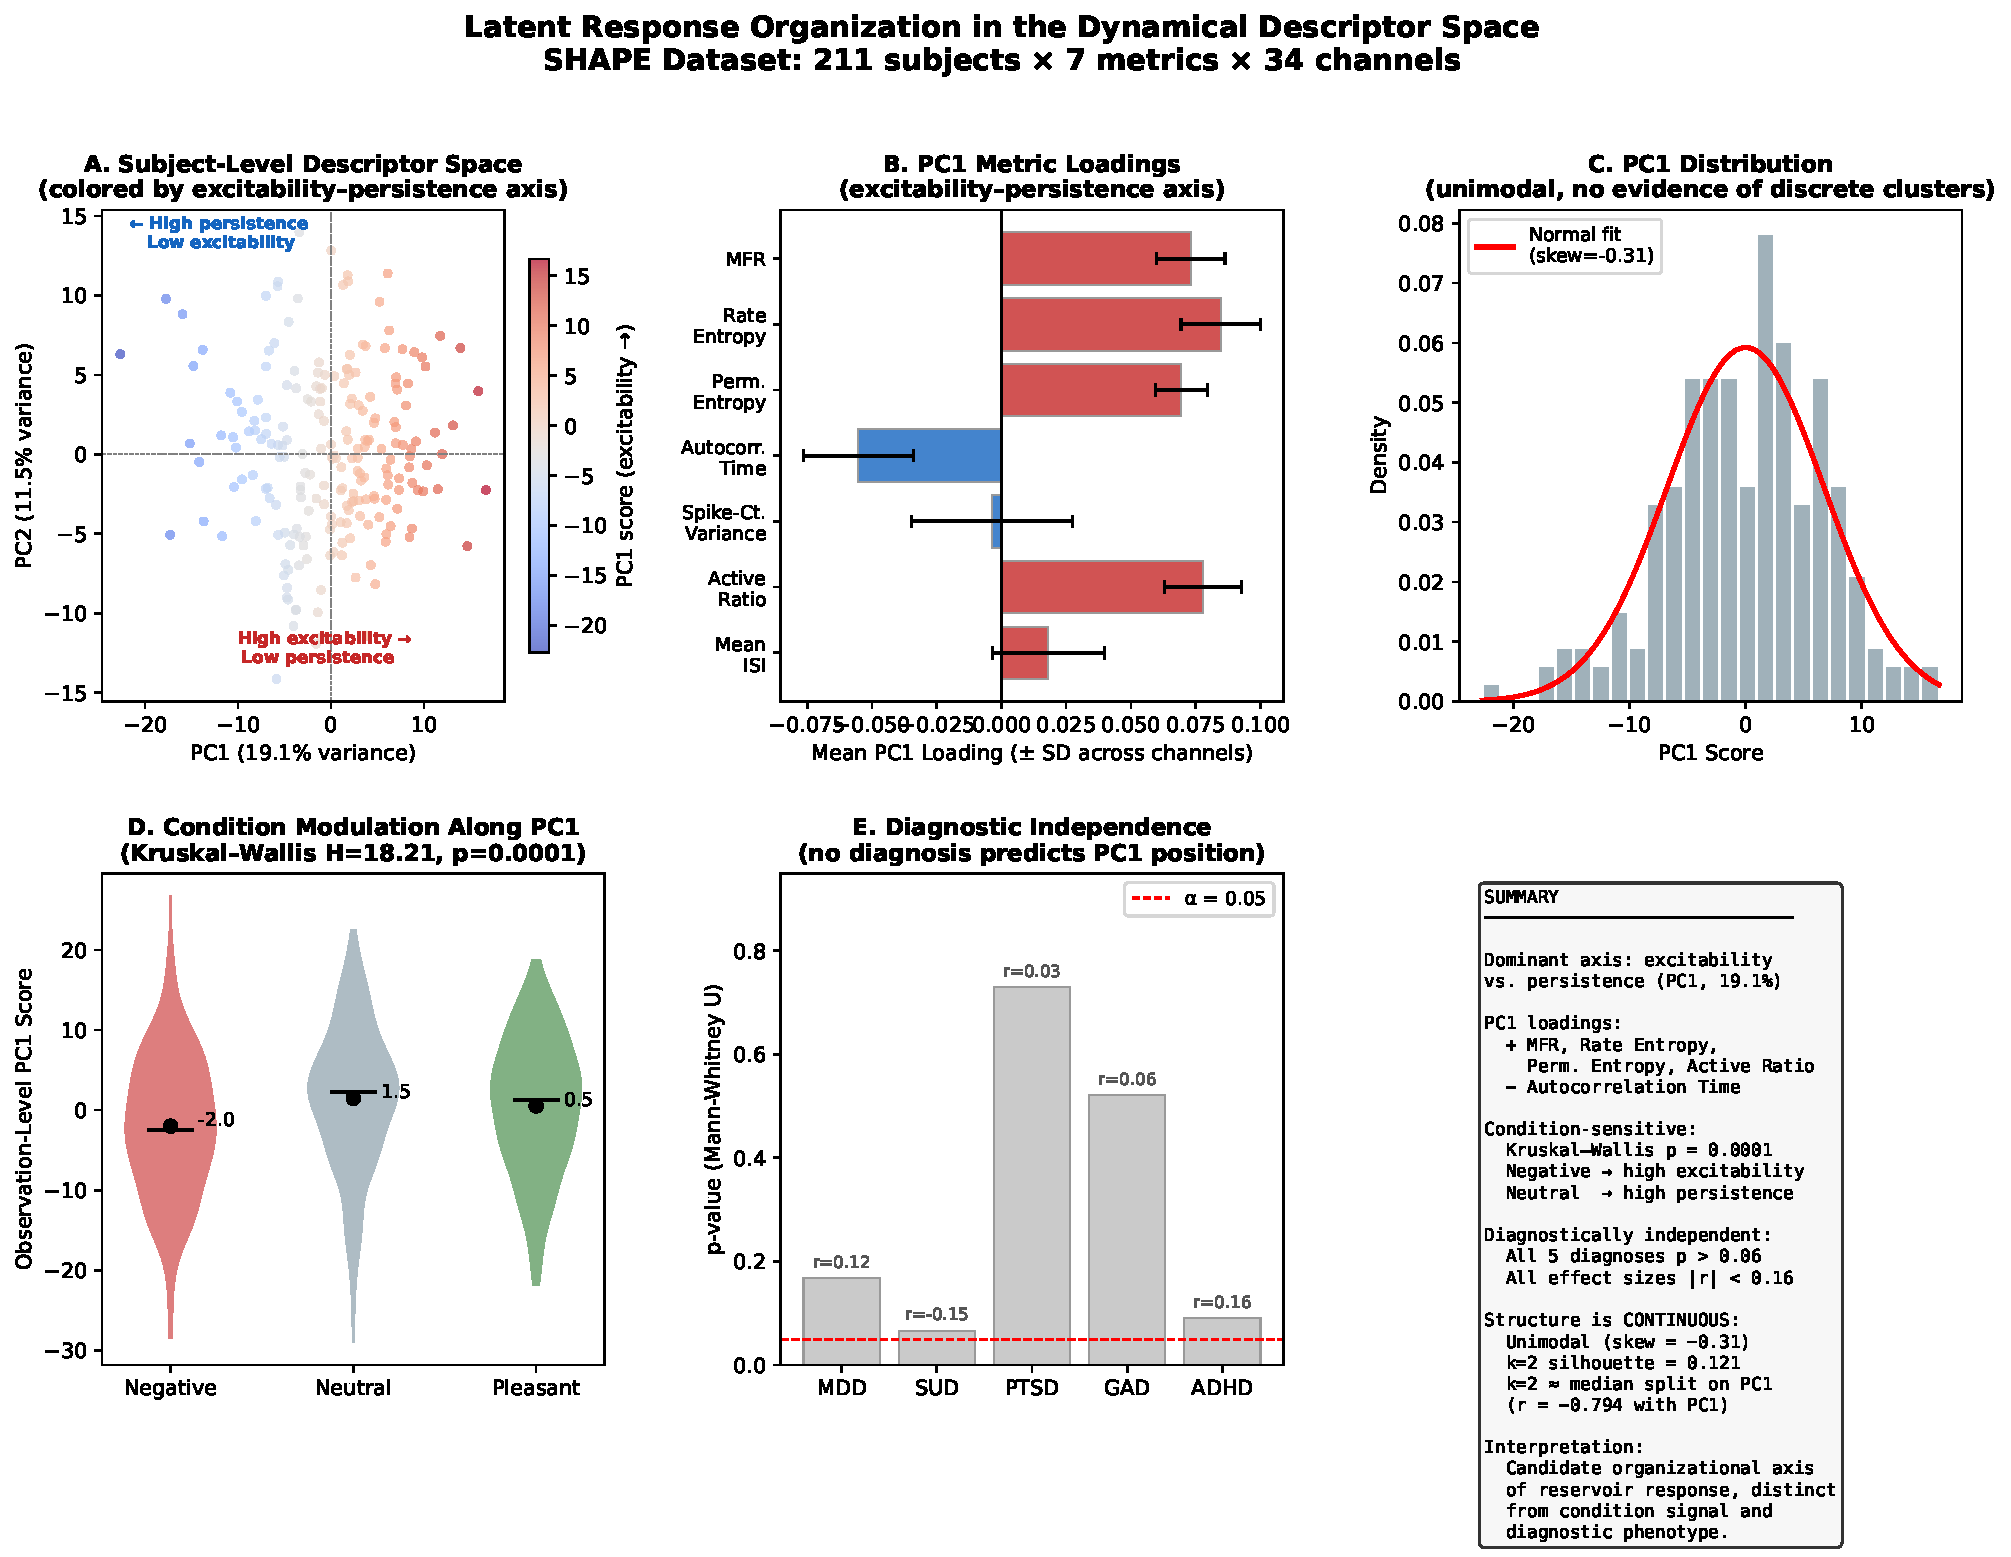
\includegraphics[width=\textwidth]{pictures/chDynamics/fig_latent_axis.pdf}
    \end{column}
    \begin{column}{0.45\textwidth}\small
      The seven descriptors organize along one continuous axis ---
      excitability--persistence (PC1, $19.1\%$):
      \begin{itemize}\small
        \item Condition-modulated: Friedman $p = 6\times 10^{-6}$.
        \item Diagnostically near-independent.
      \end{itemize}
      \vspace{0.3em}
      A patient is \emph{located} on a continuous axis, not classified into a
      bin --- the instrument paradigm made concrete.
    \end{column}
  \end{columns}
\end{frame}

% ===============================================================
\section{Part 5 --- The Graph Propagation Regime}
% ===============================================================

\begin{frame}{Layer C --- the graph question}
  \vspace{0.6em}
  Message-passing GNNs became dominant for EEG without characterization
  on the graphs EEG actually produces.
  \vspace{0.8em}
  \begin{itemize}
    \item $\leq 64$ channels
    \item $>10\%$ density
    \item $<1{,}000$ samples
  \end{itemize}
  \vspace{0.6em}
  \begin{center}\color{sbnavy}
    An open empirical question --- not a settled methodology.
  \end{center}
\end{frame}

\begin{frame}{The propagation operator}
  \vspace{0.4em}
  \begin{equation*}
    \mathbf{H}^{(k+1)} = \sigma\!\big(\mathbf{W}^{(k)}\, \tilde{\mathbf{A}}\, \mathbf{H}^{(k)}\big)
  \end{equation*}
  \begin{center}
    $\tilde{\mathbf{A}} = \mathbf{D}^{-1/2}(\mathbf{A}+\mathbf{I})\mathbf{D}^{-1/2}$
  \end{center}
  \vspace{0.6em}
  \begin{center}\color{sbaccent}
    Repeated $\tilde{\mathbf{A}}^k$ = diffusion on the graph Laplacian.\\
    Oversmoothing on dense graphs.
  \end{center}
\end{frame}
\begin{frame}{Defense audit: memory-capacity regime for leak $\beta$}
  \begin{columns}[T]
    \begin{column}{0.62\textwidth}
      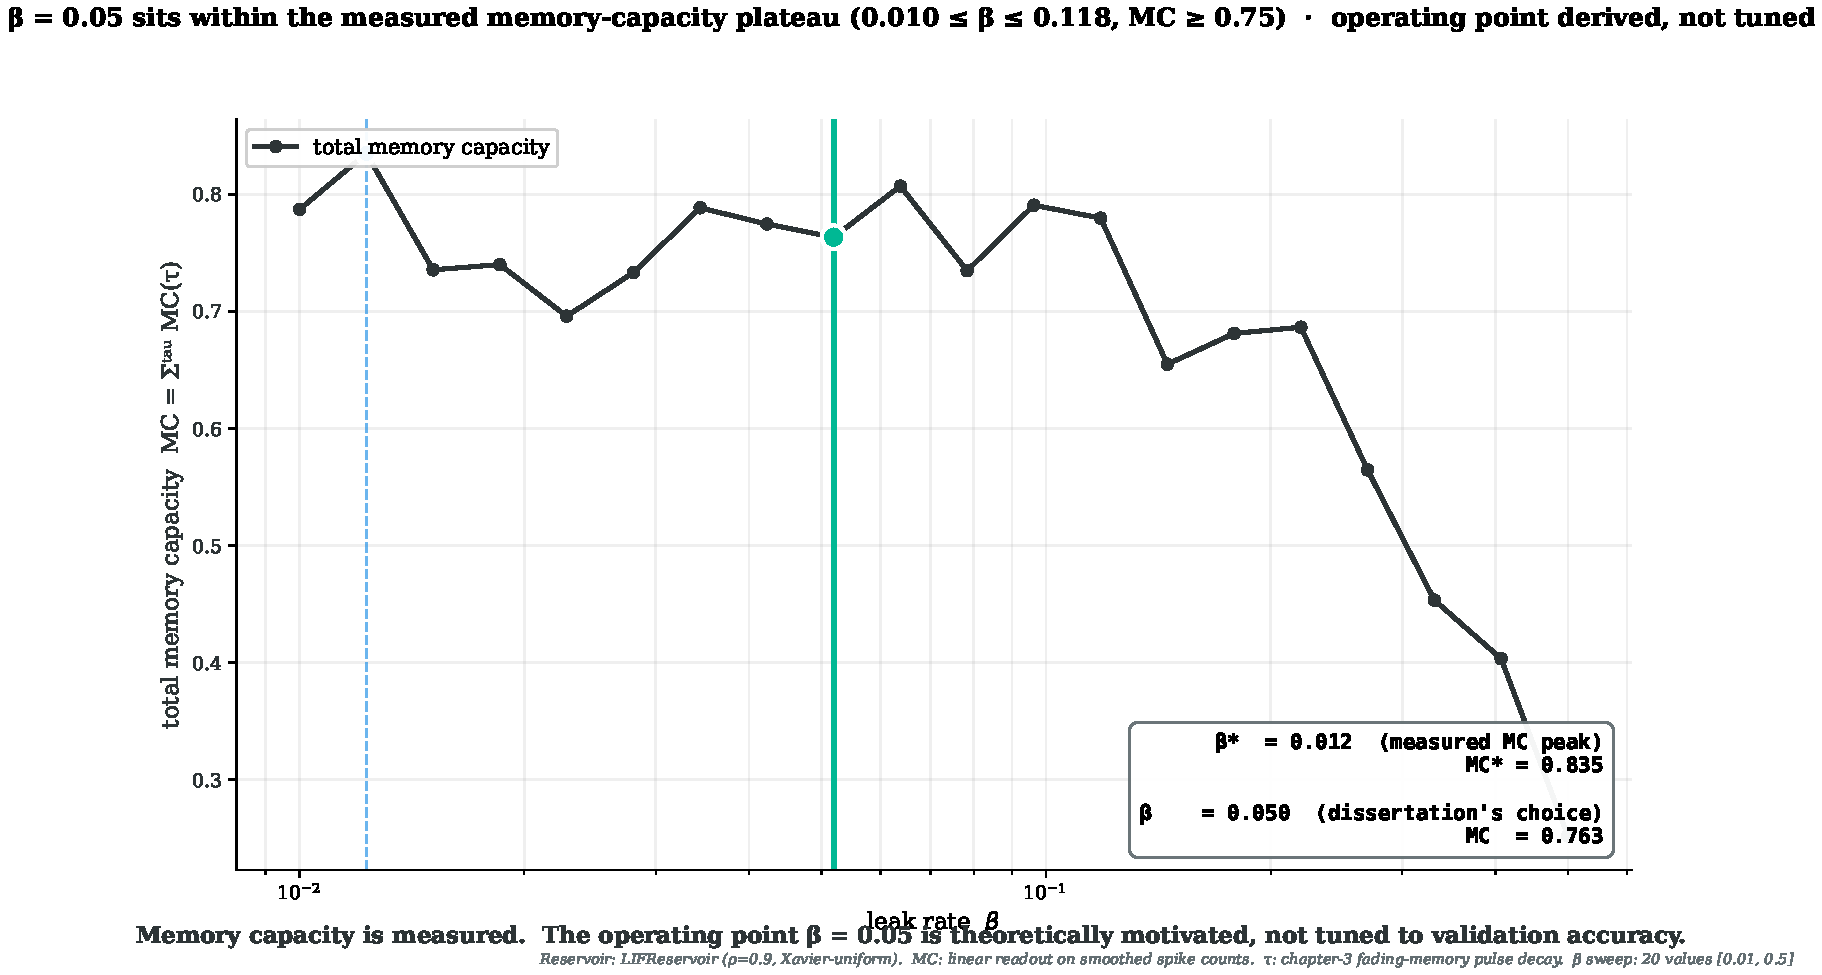
\includegraphics[width=\textwidth]{pictures/defense_audit/analysisC_3d_memory_capacity_peak.pdf}
    \end{column}
    \begin{column}{0.38\textwidth}\small
      A measured operating characteristic for the leak. $\beta = 0.05$
      sits inside the MC plateau but \alert{not} at the measured peak
      ($\beta^{*} \approx 0.012$).
      \vspace{0.4em}
      \begin{itemize}\small
        \item $\beta = 0.05 \to \mathrm{MC} \approx 0.763$ ($91\%$ of peak).
        \item Plateau $\beta \in [0.010, 0.118]$, $\mathrm{MC} \geq 0.75$.
        \item Defended by time-constant argument vs.\ the $256$-step ERP.
      \end{itemize}
    \end{column}
  \end{columns}
\end{frame}

\begin{frame}{The Propagation Operating Characteristic (Contribution 1)}
  \begin{columns}[T]
    \begin{column}{0.6\textwidth}
      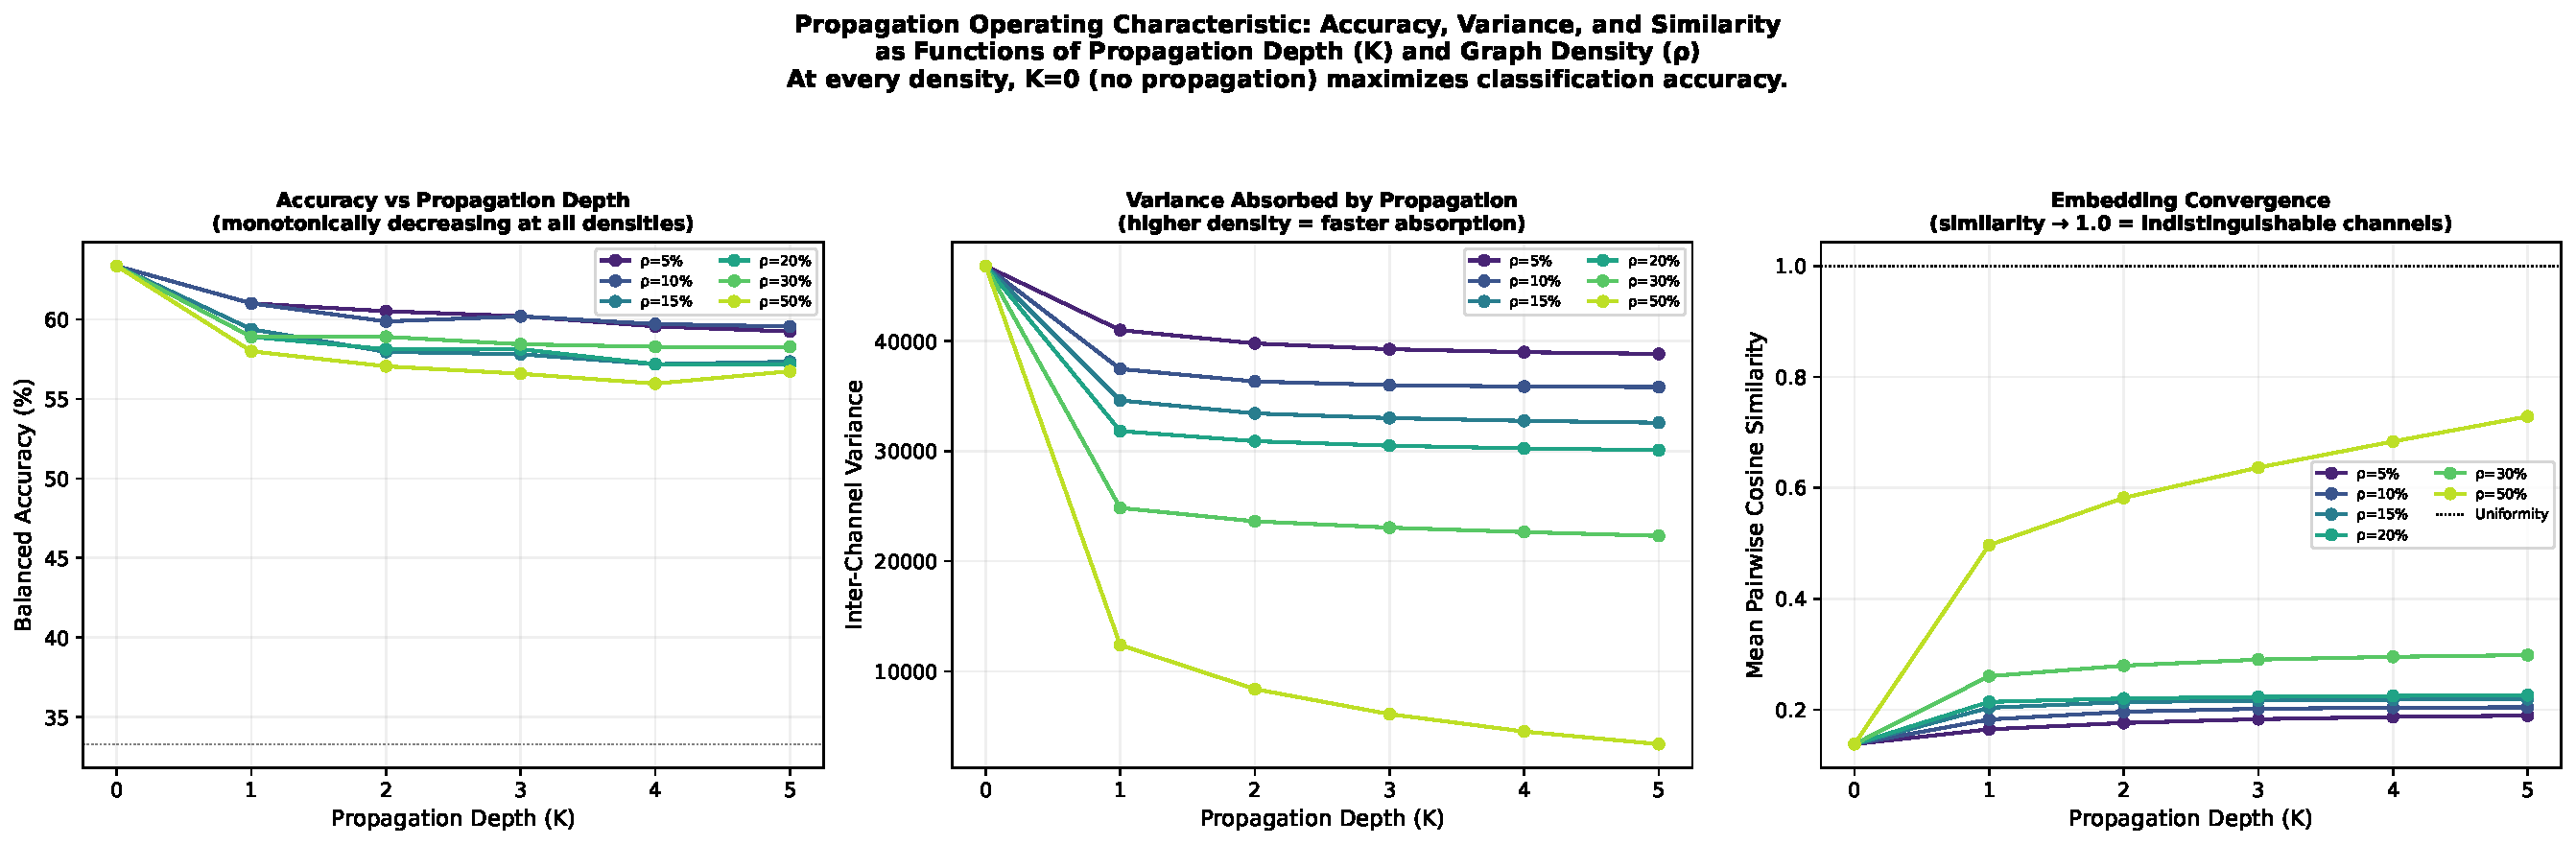
\includegraphics[width=\textwidth]{pictures/chGraphNeuralNetworks/exp03_propagation_operating_characteristic.pdf}
    \end{column}
    \begin{column}{0.4\textwidth}\small
      Across the operating characteristic, message passing
      \alert{underperforms} the non-propagated embedding at every density and
      depth.
      \vspace{0.3em}

      Design criterion: for sensor graphs $<50$ nodes and $>15\%$ density,
      smoothing-based propagation costs more inter-channel contrast than it
      contributes relational information.
    \end{column}
  \end{columns}
\end{frame}

\begin{frame}{The result is robust across graph construction}
  \begin{columns}[T]
    \begin{column}{0.6\textwidth}
      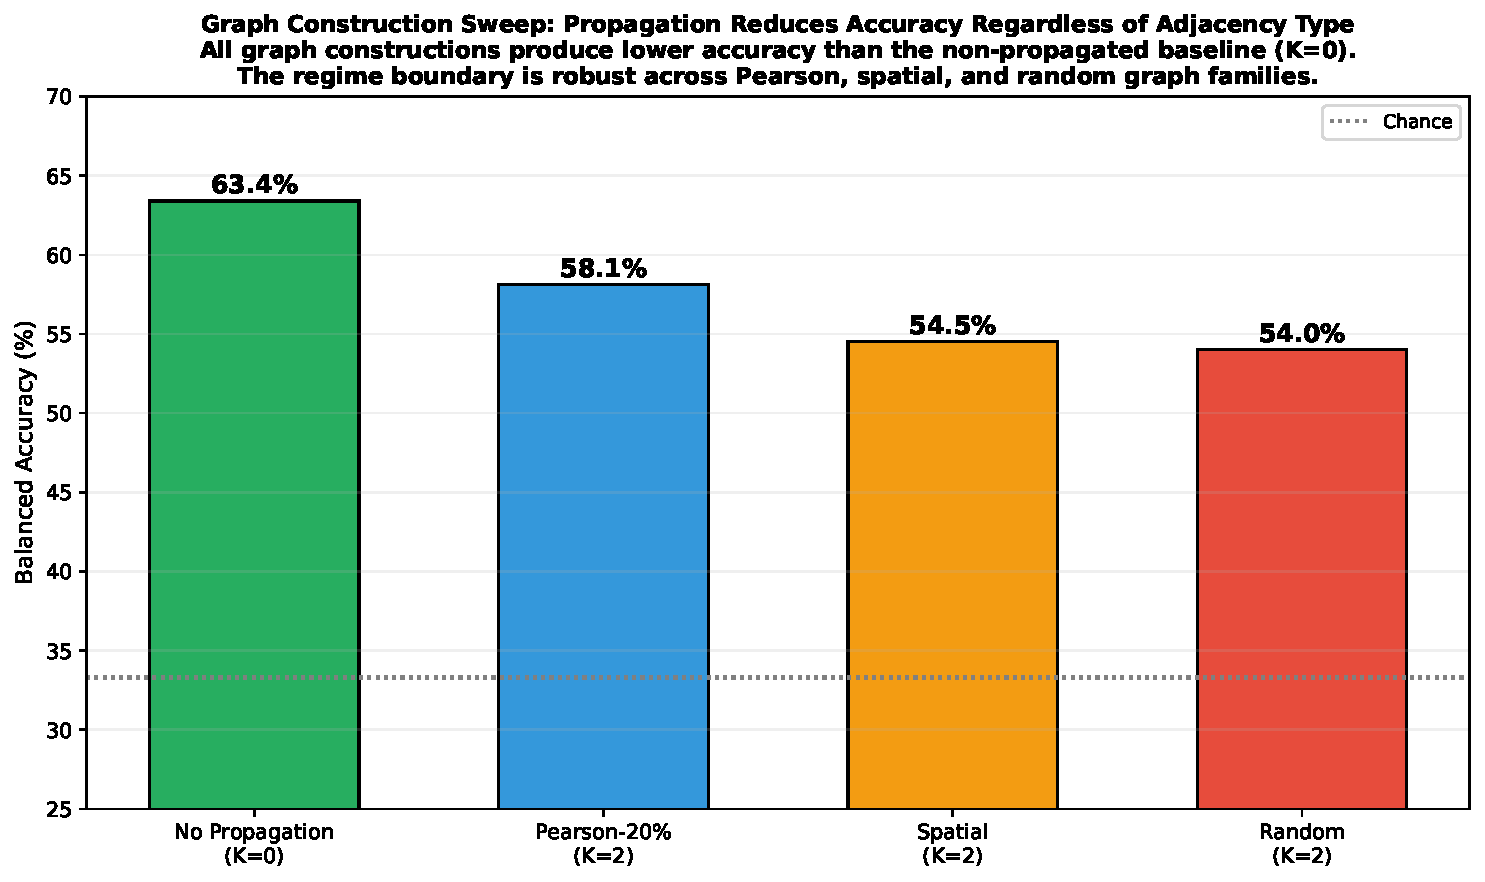
\includegraphics[width=\textwidth]{pictures/chGraphNeuralNetworks/exp04_graph_construction_sweep.pdf}
    \end{column}
    \begin{column}{0.4\textwidth}\small
      Sweeping adjacency construction (correlation, distance, functional) and
      density confirms the boundary is a property of the \emph{data regime},
      not one badly chosen graph.
      \vspace{0.3em}

      The Propagation Operating Characteristic is a tool the EEG-GNN
      literature lacked.
    \end{column}
  \end{columns}
\end{frame}

\begin{frame}{The diffusion mechanism, measured on real reservoir features}
  \begin{columns}[T]
    \begin{column}{0.6\textwidth}
      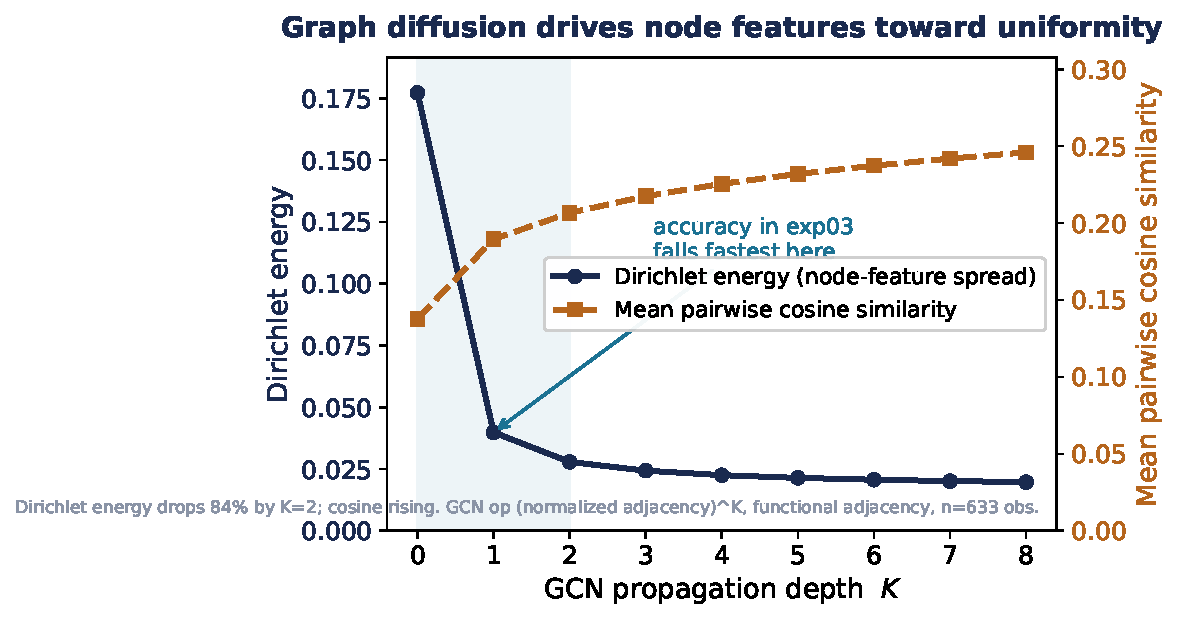
\includegraphics[width=\textwidth]{pictures/chGraphNeuralNetworks/exp03b_diffusion_overlay.pdf}
    \end{column}
    \begin{column}{0.4\textwidth}\small
      Measured on the actual reservoir node features ($n=633$, verbatim repo
      operators):
      \begin{itemize}\small
        \item Dirichlet energy drops \alert{$84\%$ by $K=2$}.
        \item Mean pairwise cosine similarity rises toward uniformity.
      \end{itemize}
      \vspace{0.3em}
      Exactly the regime where accuracy in \texttt{exp03} falls fastest. A
      mechanistic correlate of the observed boundary.
    \end{column}
  \end{columns}
\end{frame}
\begin{frame}{Defense audit: theoretical bounds vs.\ measured operating points}
  \centering
  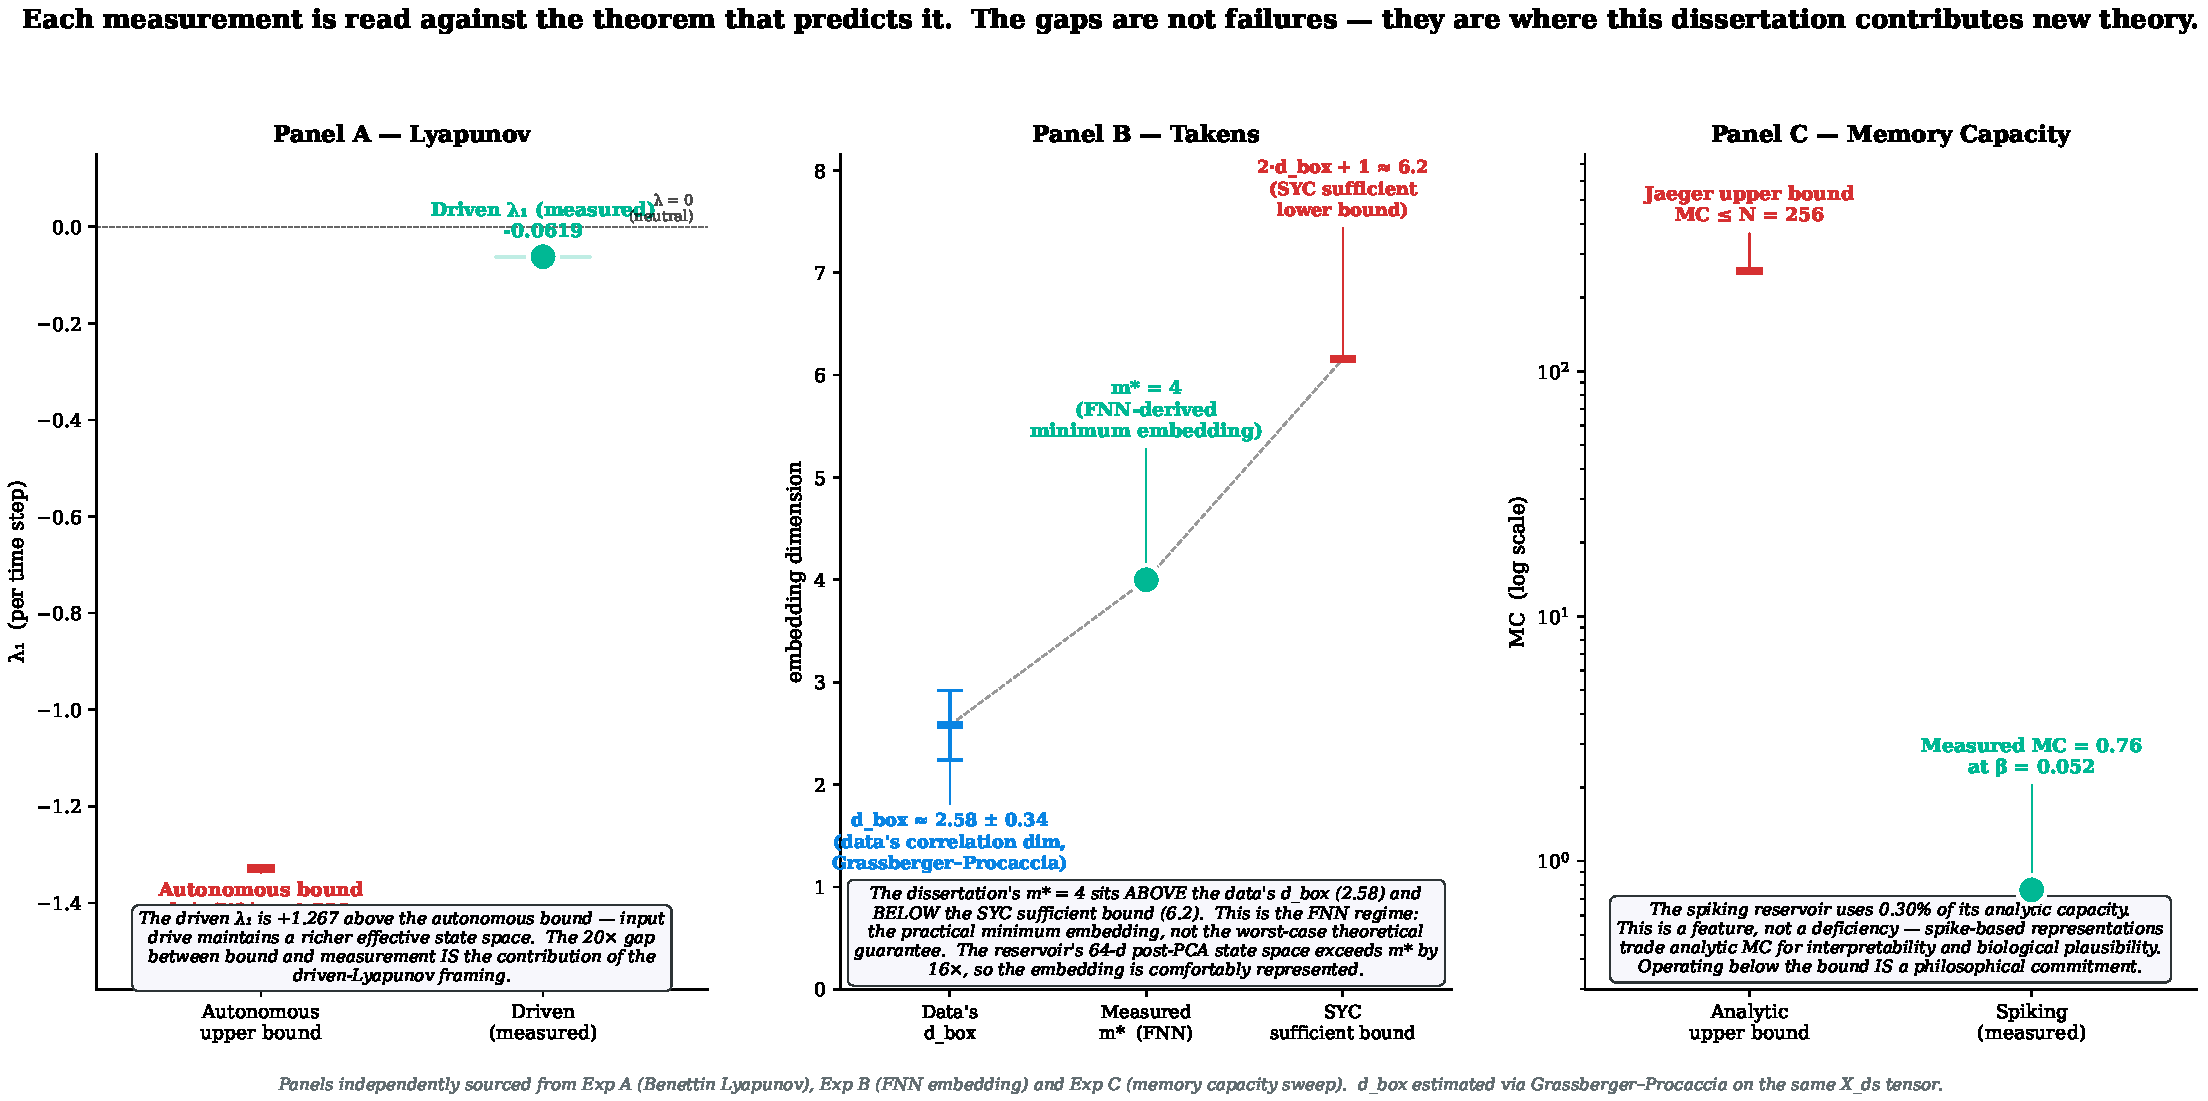
\includegraphics[width=\textwidth,height=0.80\textheight,keepaspectratio]{pictures/defense_audit/analysisTB_5a_bounds_vs_measurement.pdf}
\end{frame}

\begin{frame}{Reframing the graph layer}
  \vspace{1.2em}
  \begin{center}\large
    \textbf{Not} a propagation-based classifier.\\[0.6em]
    \textbf{Instead} a Level-4 phenotyping instrument.
  \end{center}
  \vspace{1.2em}
  \begin{center}\color{sbnavy}
    The graph is a structural lens --- and feeds the coupling analysis.
  \end{center}
\end{frame}

\begin{frame}{Structure--function coupling, $\kappa$}
  For each subject and condition, the coupling matrix collects electrode-wise
  Spearman correlations between the seven dynamical and the topological
  descriptor families:
  \begin{equation*}
    \kappa_{s,c} = \frac{\|\mathbf{C}_{s,c}\|_F}{\sqrt{p\cdot q}}
      = \frac{1}{\sqrt{14}}\sqrt{\sum_{j=1}^{7}\sum_{k=1}^{2}(\mathbf{C}_{s,c})_{jk}^2}.
  \end{equation*}
  $\kappa \to 0$: families unaligned. $\kappa \to 1$: every dynamical
  descriptor rank-correlates with every topological descriptor. $\kappa$ is
  itself the interpretable observable.
\end{frame}

\begin{frame}{Coupling is real above the permutation null}
  \begin{columns}[T]
    \begin{column}{0.55\textwidth}\centering
      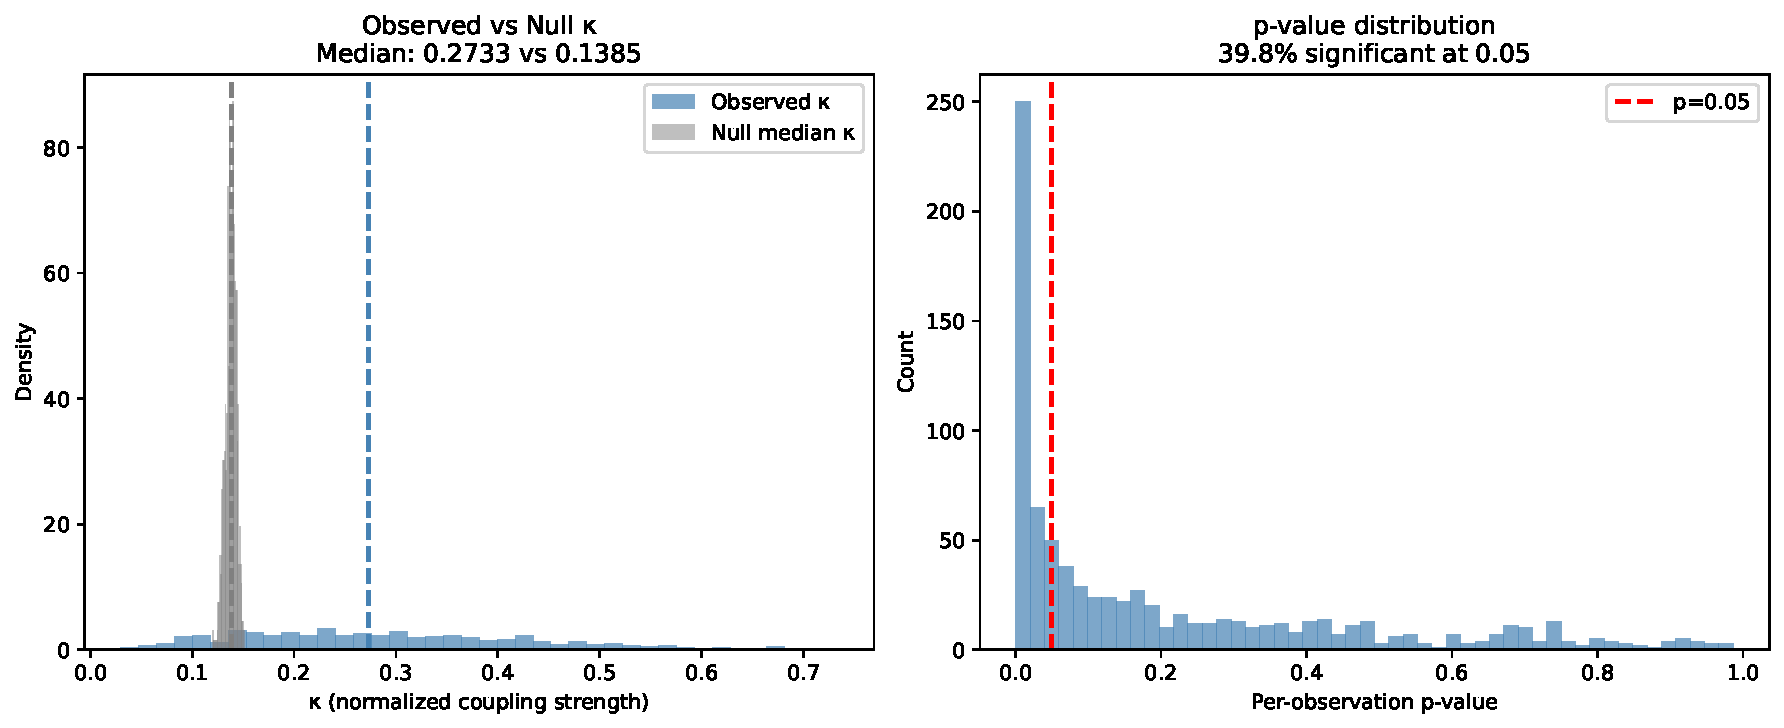
\includegraphics[width=\textwidth]{pictures/chSynthesis/fig7_A2_kappa_vs_null.pdf}
    \end{column}
    \begin{column}{0.45\textwidth}\small
      Against an electrode-permutation null: median $\kappa = 0.273$.
      \begin{alertblock}{Subject-level inference}
        \small Confirmed at the subject level ($N=211$, one-sample Wilcoxon,
        $p < 0.001$).
      \end{alertblock}
      Temporal dynamics and spatial topology are systematically related ---
      the pipeline describes one coherent system.
    \end{column}
  \end{columns}
\end{frame}

% ===============================================================
\section{Part 6 --- Intrinsic Interpretability}
% ===============================================================

\begin{frame}{Post-hoc vs.\ intrinsic interpretability}
  \vspace{0.4em}
  \begin{columns}[T]
    \begin{column}{0.5\textwidth}
      \textbf{Post-hoc}
      \begin{itemize}
        \item Explanation generated \emph{after} training.
        \item Approximates what the model attended to.
        \item Inherits the model's biases.
      \end{itemize}
    \end{column}
    \begin{column}{0.5\textwidth}
      \textbf{Intrinsic}
      \begin{itemize}
        \item Intermediate variables \emph{are} the explanation.
        \item Named physical interpretation.
        \item Validated independently.
      \end{itemize}
    \end{column}
  \end{columns}
  \vspace{0.6em}
  \begin{center}\color{sbnavy}
    Intrinsic interpretability requires no second model.
  \end{center}
\end{frame}

\begin{frame}{The four-level taxonomy --- measured}
  \centering\small
  \vspace{0.4em}
  \begin{tabular}{lll}\toprule
    \textbf{Level} & \textbf{Observable} & \textbf{Measured} \\\midrule
    L1 Temporal     & bin vs.\ ERP scalar            & $|r| = 0.82$ (LPP) \\
    L2 Geometric    & subject vs.\ condition variance & $\rho = 7.2$; $+13$--$21$\,pp \\
    L3 Dynamical    & descriptor vs.\ ERP scalar      & $|r|$ up to $0.84$ \\
    L4 Coupling     & $\kappa$ vs.\ permutation null  & $0.273$, $p<0.001$ \\
    \bottomrule
  \end{tabular}
  \vspace{0.6em}\\
  \normalsize\color{sbnavy}
  First architecture interpretable at \emph{all four levels} in one pipeline.
\end{frame}

\begin{frame}{What interpretability enables}
  \vspace{0.6em}
  Centering moves \alert{every} model $+13$ to $+21$\,pp.
  \vspace{0.6em}
  \begin{itemize}
    \item Hidden condition order was in the signal all along.
    \item Buried under subject geometry at $\rho=7.2$.
    \item Recoverable across every tested architecture.
  \end{itemize}
  \vspace{0.6em}
  \begin{center}\color{sbnavy}
    Level-2 transparency made the discovery visible.\\
    A black box never would have.
  \end{center}
\end{frame}

\begin{frame}{A theoretically predicted null}
  \vspace{0.4em}
  \begin{center}\large
    PCA-64 after centering: chance accuracy.
  \end{center}
  \vspace{0.6em}
  Principal-angle analysis:
  \begin{itemize}
    \item Subject \& condition subspaces: principal angles $= 0^\circ$.
    \item Cosine alignment $= 1.000$.
    \item Centering \emph{must} project condition with subject.
  \end{itemize}
  \vspace{0.4em}
  \begin{center}\color{sbnavy}
    Not a bug --- predicted by the framework's own geometry.
  \end{center}
\end{frame}

\begin{frame}{A null result that forced the methodology}
  \vspace{0.6em}
  Channel-averaged: \alert{0 / 49} significant comparisons.
  \vspace{0.4em}
  \begin{center}\large
    Standard reading: close the chapter.
  \end{center}
  \vspace{0.4em}
  Interpretability framework asked: \emph{what if it needs spatial resolution?}
  \vspace{0.6em}
  Per-channel reanalysis:
  \begin{itemize}
    \item SUD: \textbf{53.6\%} --- strongest in the entire ablation matrix.
    \item PTSD: \textbf{52.6\%}.
  \end{itemize}
  \vspace{0.2em}
  \begin{center}\color{sbnavy}\small
    The layer-specific finding does not exist without this null.
  \end{center}
\end{frame}
\begin{frame}{Defense audit: per-trial channel-permutation null}
  \begin{columns}[T]
    \begin{column}{0.62\textwidth}
      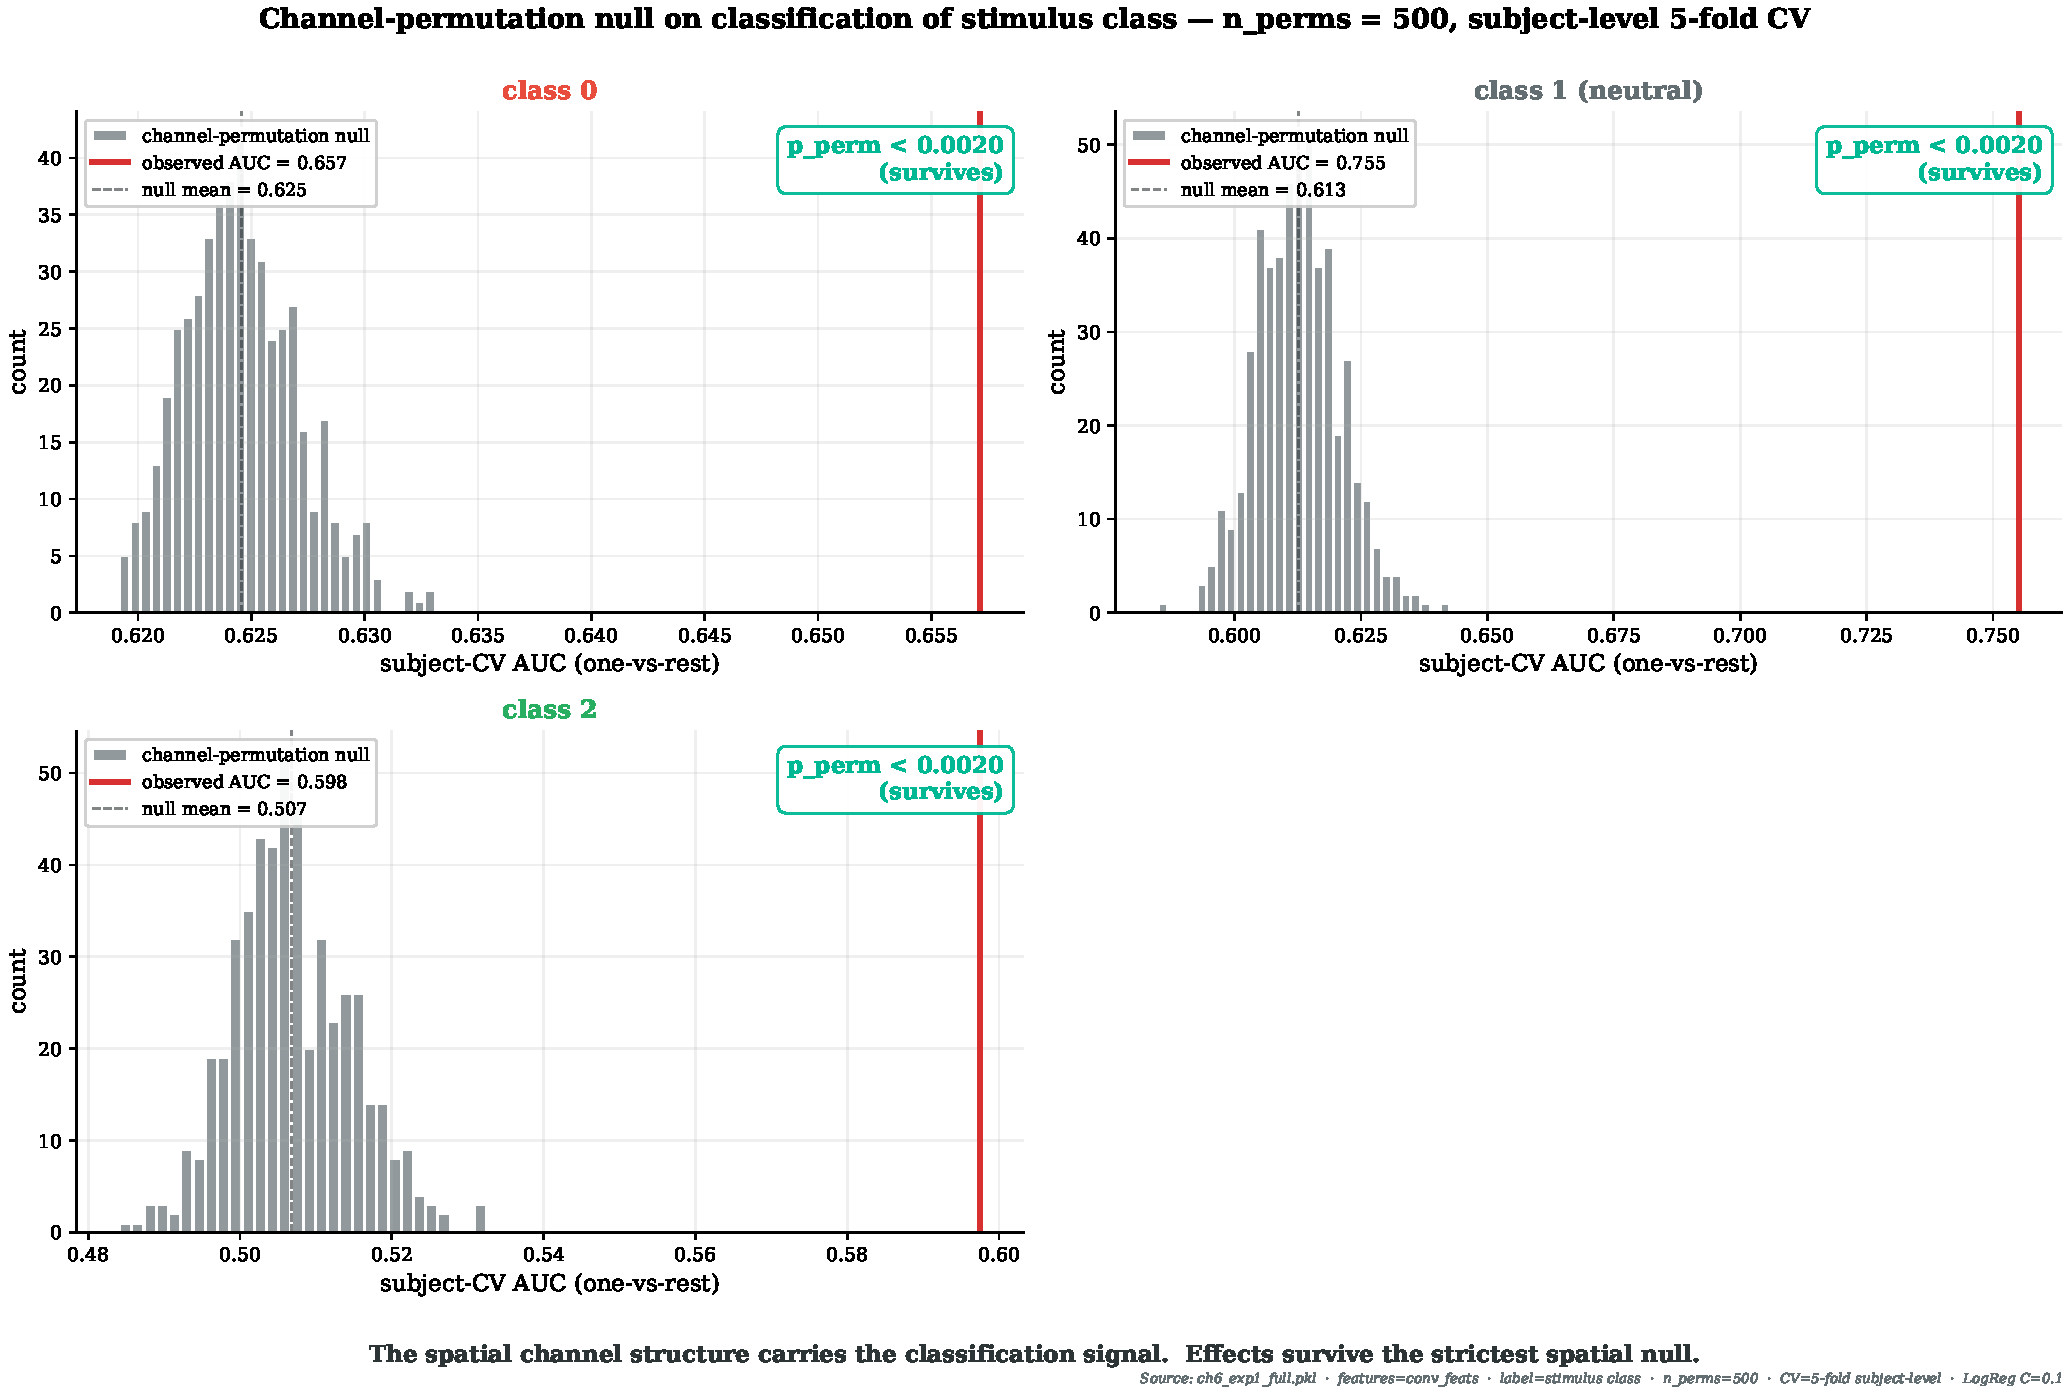
\includegraphics[width=\textwidth]{pictures/defense_audit/analysisD_4d_permutation_nulls.pdf}
    \end{column}
    \begin{column}{0.38\textwidth}\small
      The strictest spatial null: an independent permutation $\pi_i$
      \alert{per trial}, not one global $\pi$. A flat classifier cannot
      compensate.
      \vspace{0.4em}
      \begin{itemize}\small
        \item $500$ perms $\times$ $5$ CV folds, subject-level.
        \item Stimulus-class --- not a clinical-disorder claim.
        \item CLI flag swaps to disorder labels when CSV is supplied.
      \end{itemize}
    \end{column}
  \end{columns}
\end{frame}

\begin{frame}{Defense audit: failure gallery --- four pivots}
  \centering
  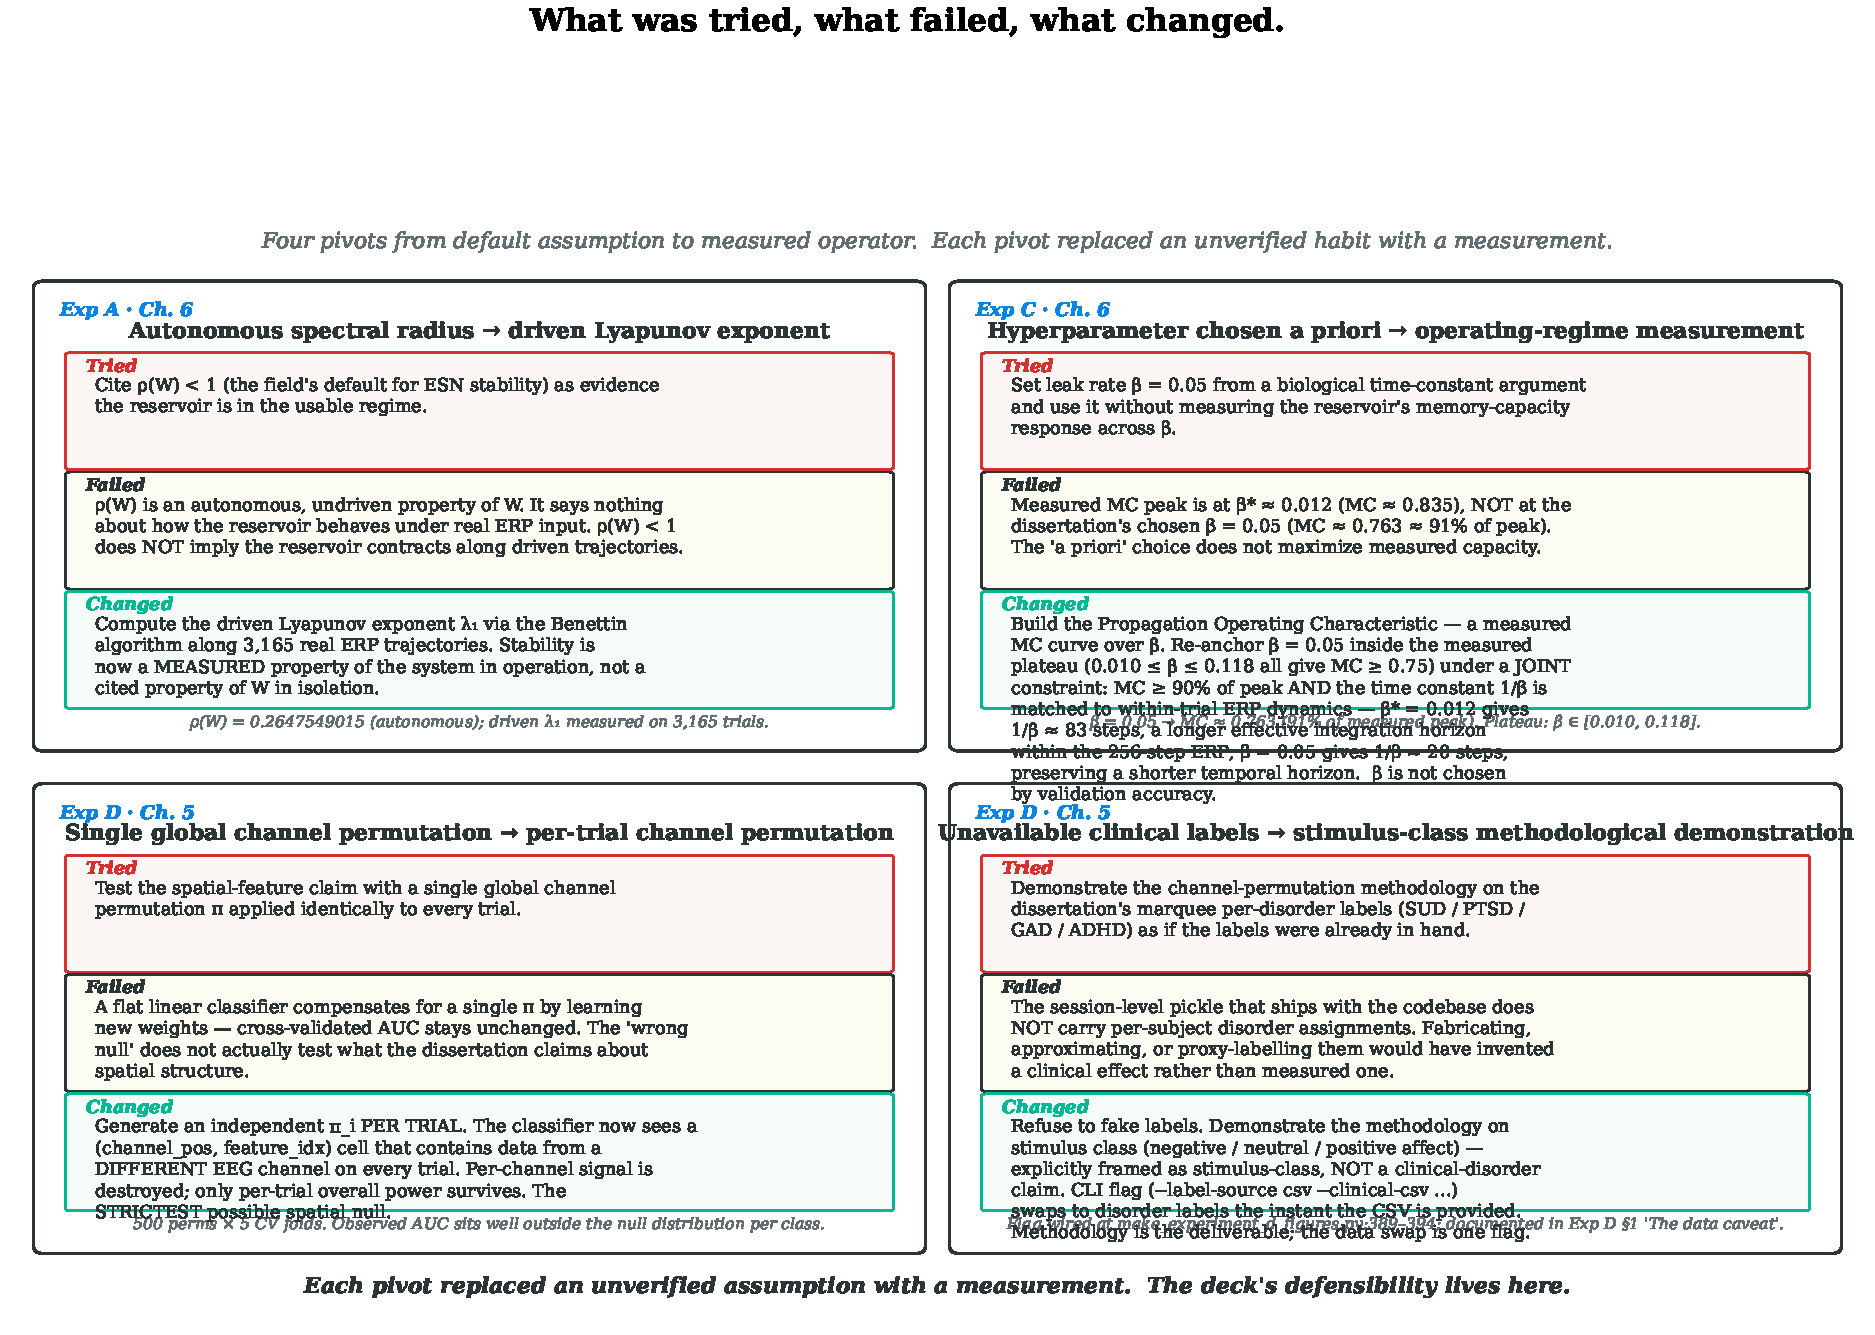
\includegraphics[width=\textwidth,height=0.85\textheight,keepaspectratio]{pictures/defense_audit/figG_failure_gallery.pdf}
\end{frame}

\begin{frame}{Different disorders, different layers}
  \vspace{0.4em}
  \centering\small
  \begin{tabular}{lll}\toprule
    \textbf{Disorder} & \textbf{Layer} & \textbf{$p$} \\\midrule
    SUD  & Dynamical descriptors & $0.0004$ \\
    PTSD & Dynamical descriptors & $0.036$ \\
    GAD  & Graph topology        & $0.032$ \\
    ADHD & Cross-layer coupling  & --- \\
    \bottomrule
  \end{tabular}
  \vspace{0.8em}\\
  \normalsize\color{sbnavy}
  Only a four-level framework can produce this profile.
  \vspace{0.2em}\\
  {\scriptsize\color{gray} Exploratory, hypothesis-generating; pending independent replication.}
\end{frame}

\begin{frame}{Layer ablation methodology (Contribution 4)}
  Complementarity is tested directly, not asserted.
  \begin{columns}[T]
    \begin{column}{0.55\textwidth}\centering
      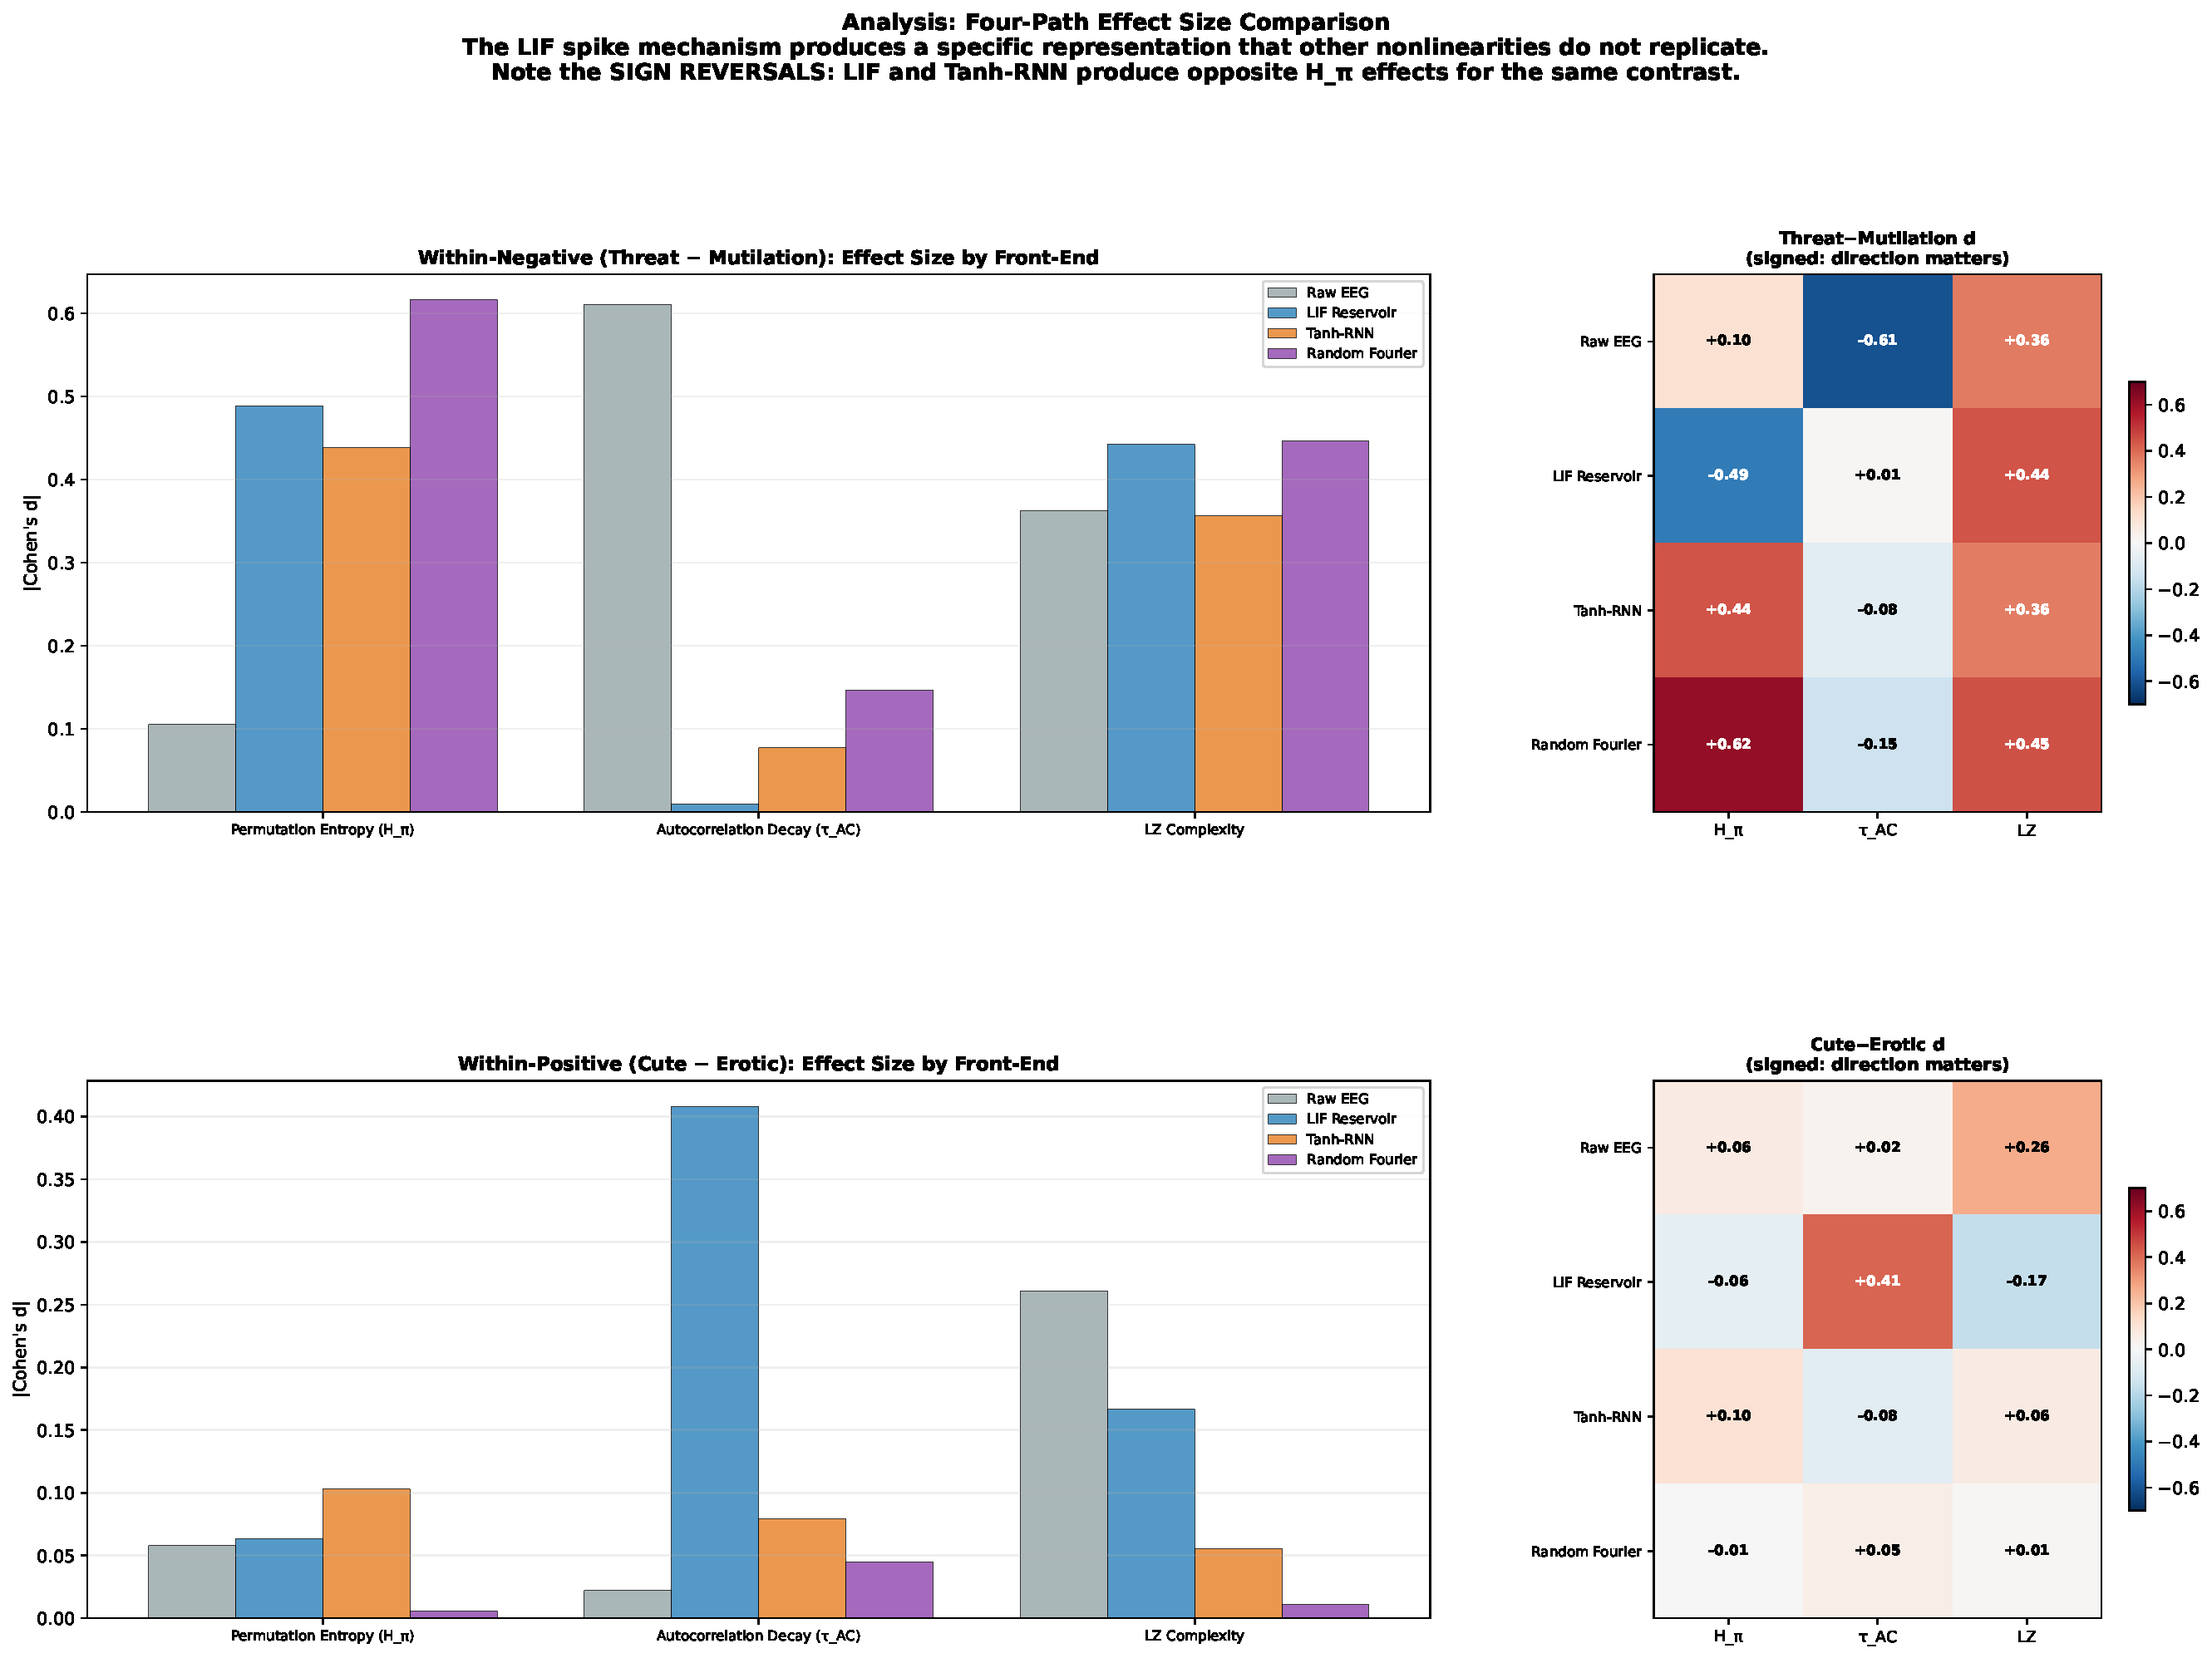
\includegraphics[width=\textwidth]{pictures/chDynamics/analysis6_3_four_path_comparison.pdf}\\
      \srccap{Four-path comparison across processing routes}
    \end{column}
    \begin{column}{0.45\textwidth}\small
      Methodology rule: linear-readout content comparison exposes geometric
      separability without classifier rescue. Cross-disorder profiling tests
      whether layers carry redundant or complementary information.
      \vspace{0.3em}

      \alert{Result:} layers are complementary, not redundant. Combining
      temporal and spatial features never improves classification beyond the
      better individual family --- but each disorder is detected by a
      different family.
    \end{column}
  \end{columns}
\end{frame}

\begin{frame}{The accuracy--interpretability trade}
  \vspace{0.6em}
  \begin{center}\large
    ARSPI-Net: \textbf{78.8\%} + full decomposition.\\[0.4em]
    EEGNet: \textbf{89.1\%} + no inspectable intermediate.
  \end{center}
  \vspace{0.6em}
  \begin{itemize}
    \item Matches GRU ($78.4\%$) --- zero trainable recurrent parameters.
    \item Exceeds LSTM ($71.1\%$).
  \end{itemize}
  \vspace{0.4em}
  \begin{center}\color{sbnavy}
    The trade \emph{is} the contribution.
  \end{center}
\end{frame}

% ===============================================================
\section{Part 7 --- Scope, Future, and Close}
% ===============================================================

\begin{frame}{Scope of validation}
  \vspace{0.6em}
  \begin{itemize}
    \item \textbf{Cohort.} SHAPE, $N=211$, transdiagnostic adults.
    \item \textbf{Inference.} Subject-level; subject-disjoint CV.
    \item \textbf{Clinical.} Exploratory; permutation tested.
    \item \textbf{Energy.} Motivational; on-chip is future work.
  \end{itemize}
\end{frame}

\begin{frame}{Future directions}
  \vspace{0.6em}
  \begin{itemize}
    \item On-chip --- Loihi 2 / LAVA.
    \item Single-trial processing.
    \item Trainable plastic readout + BSC ablation.
    \item Clinical replication with SHAPE Lab.
    \item Per-stimulus dimensional affect.
  \end{itemize}
\end{frame}

\begin{frame}{Contributions restated}
  \vspace{0.4em}
  \begin{enumerate}
    \item Propagation Operating Characteristic.
    \item Spike-to-embedding pipeline.
    \item Measurement-instrument paradigm.
    \item Layer ablation methodology.
    \item Centered baseline comparison.
  \end{enumerate}
  \vspace{0.8em}
  \begin{center}\color{sbnavy}
    Unified by the three-layer claim.
  \end{center}
\end{frame}

\begin{frame}{The governing question, answered}
  \vspace{0.6em}
  \begin{itemize}
    \item \textbf{Stable.} $\lambda_1 = -0.054$, 100\% negative.
    \item \textbf{Compressible.} BSC$_6$, PCA-64.
    \item \textbf{Structurally coherent.} $\kappa = 0.273$, $p < 0.001$.
    \item \textbf{Interpretable.} L1--L4 validated.
  \end{itemize}
  \vspace{1.0em}
  \begin{center}\large\color{sbaccent}
    The architecture \emph{is} the explanation.
  \end{center}
\end{frame}

\begin{frame}{Defense claims are anchored to dissertation chapters}
  \centering
  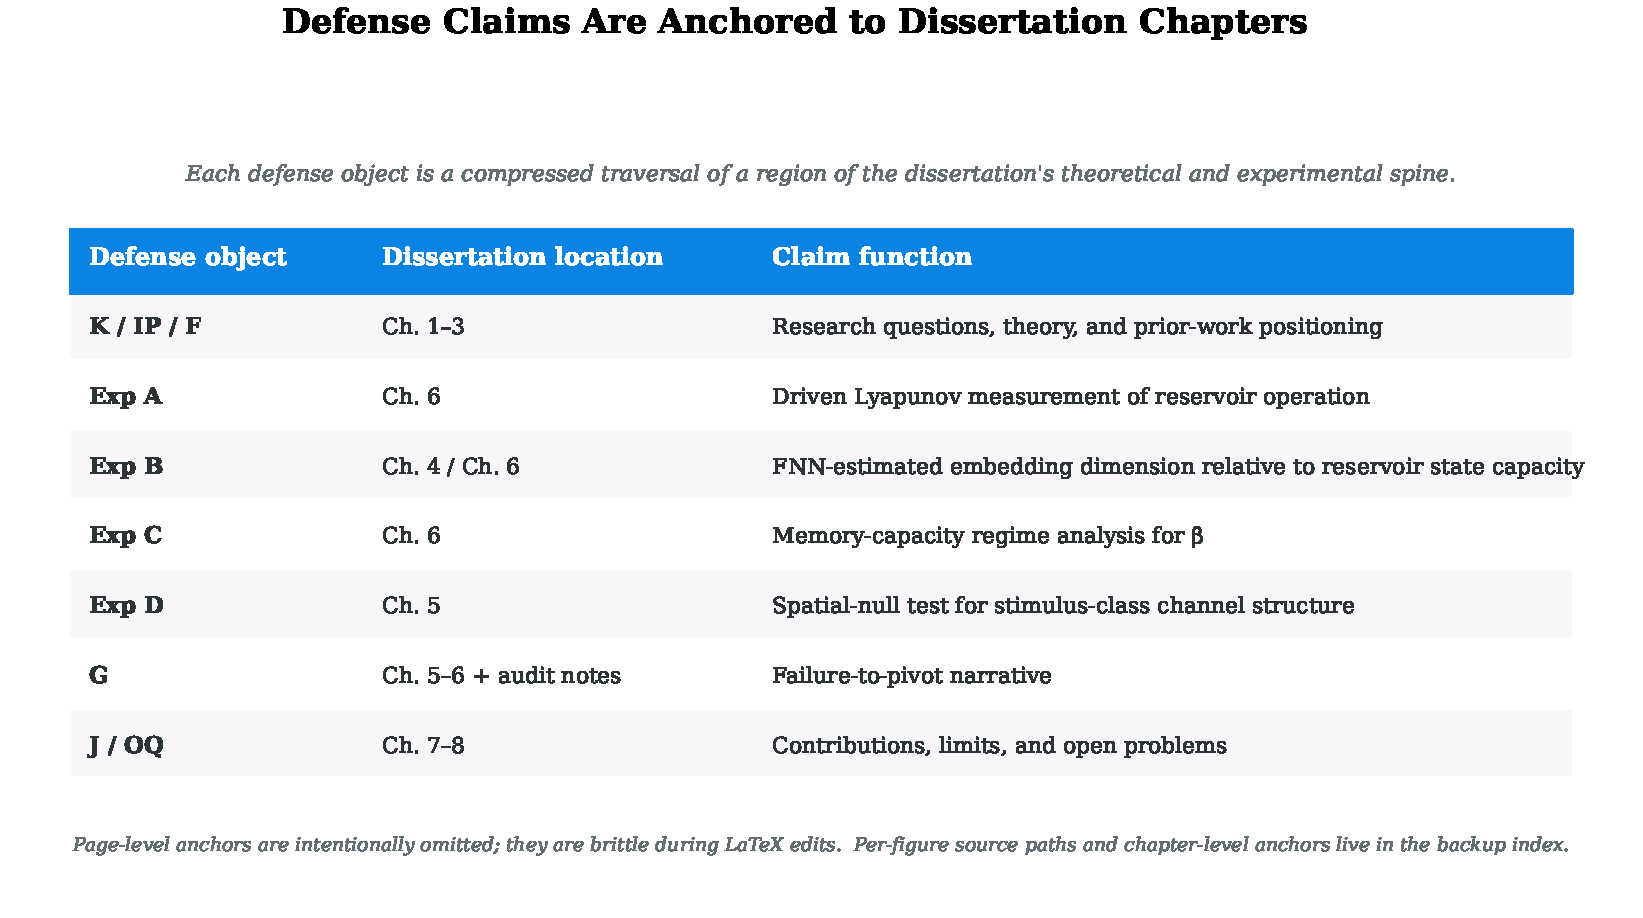
\includegraphics[width=\textwidth,height=0.82\textheight,keepaspectratio]{pictures/defense_audit/figAM_anchor_map.pdf}
\end{frame}

\begin{frame}{Research provenance and assistance}
  \centering
  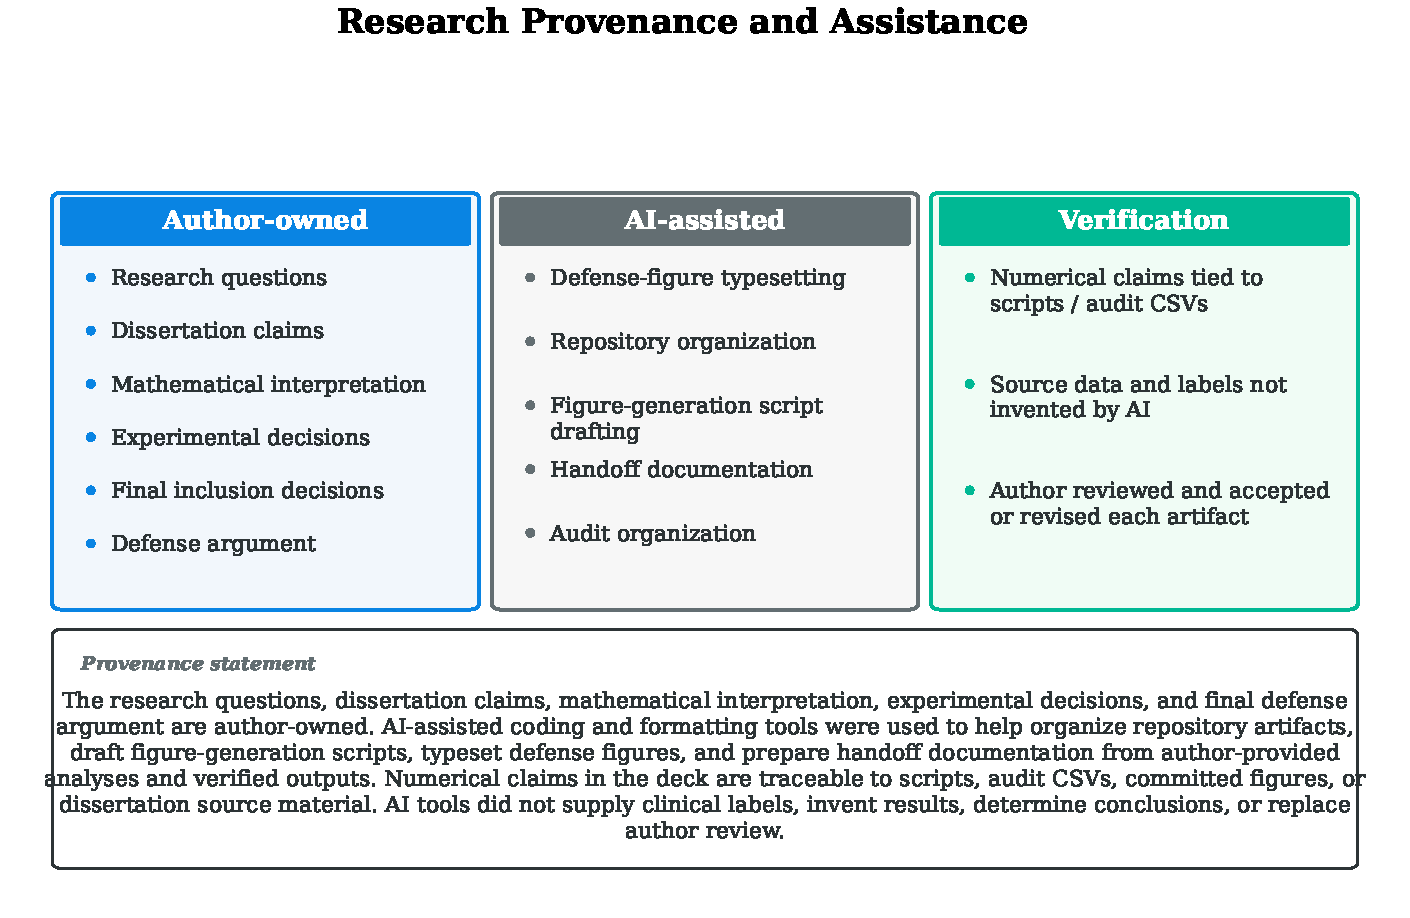
\includegraphics[width=\textwidth,height=0.82\textheight,keepaspectratio]{pictures/defense_audit/figAC_research_provenance.pdf}
\end{frame}

\begin{frame}[standout]
  Thank you.\\[0.4em]
  {\normalsize Questions and discussion.}
\end{frame}

% ===============================================================
\appendix
\section{Appendix --- Question Resources}
% ===============================================================

\begin{frame}{Appendix --- Why six temporal bins?}
  \begin{columns}[T]
    \begin{column}{0.52\textwidth}\centering
      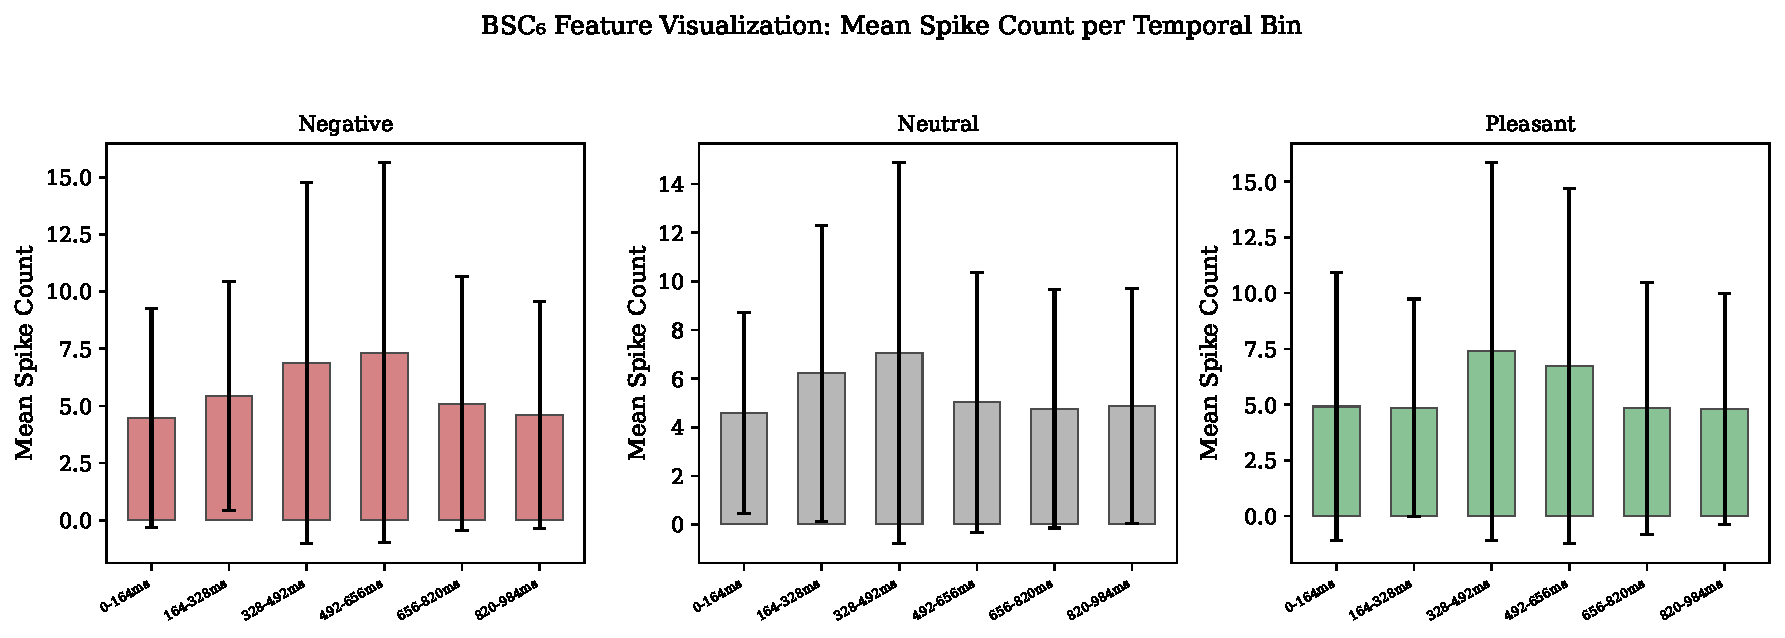
\includegraphics[width=\textwidth]{pictures/chGraphNeuralNetworks/bsc6_visualization.pdf}\\
      \srccap{$\text{BSC}_6$ temporal binning over the ERP epoch}
    \end{column}
    \begin{column}{0.48\textwidth}\small
      \begin{itemize}\small
        \item \textbf{Alignment.} Six bins resolve N1, P200, P300, LPP without
          splitting a component.
        \item \textbf{Sparsity.} Coarse enough to keep the code sparse;
          per-channel dimension tractable.
        \item \textbf{Stability.} Finer binning increases per-bin variance at
          fixed epoch length.
      \end{itemize}
      A formal bin-count ablation ($3/6/12/24$) is defined future work.
    \end{column}
  \end{columns}
\end{frame}

\begin{frame}{Appendix --- Three generations of neural computation}
  \centering\small
  \begin{tabular}{lll}\toprule
    Generation & Mechanism & Time dimension \\\midrule
    1st (McCulloch--Pitts) & Threshold logic & discrete, none \\
    2nd (deep learning) & Rate abstraction; dense synchronous & implicit \\
    3rd (Maass 1997) & Spiking; sparse asynchronous & explicit \\
    \bottomrule
  \end{tabular}
  \vspace{0.6em}

  \normalsize The third generation makes a transient-dominated signal like
  EEG a natural fit and makes the internal computation analyzable as
  \emph{dynamics}, not learned weights.
\end{frame}

\begin{frame}{Appendix --- Conventional vs.\ spiking computation}
  \begin{columns}[T]
    \begin{column}{0.5\textwidth}\centering
      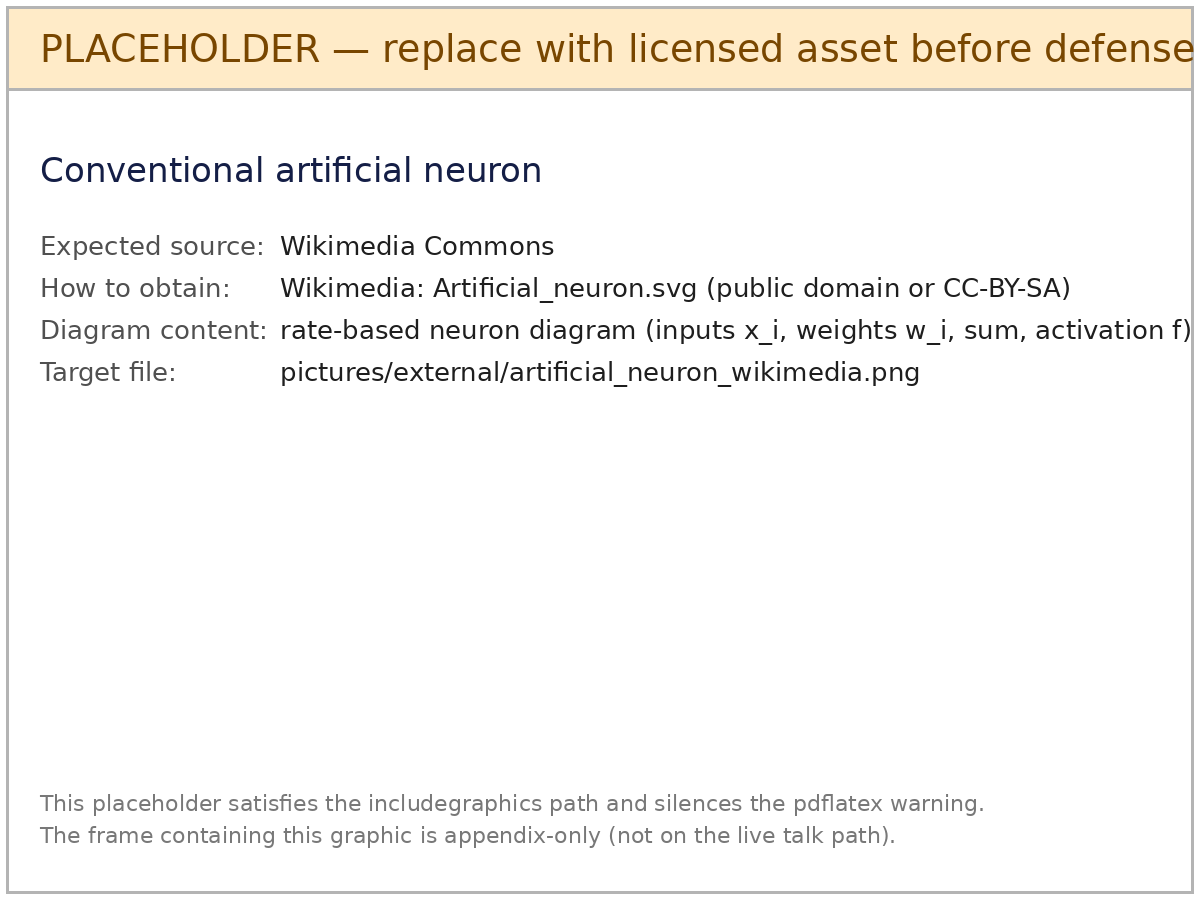
\includegraphics[width=0.92\textwidth]{pictures/external/artificial_neuron_wikimedia.png}\\
      \srccap{Conventional artificial neuron (Wikimedia Commons)}
    \end{column}
    \begin{column}{0.5\textwidth}\centering
      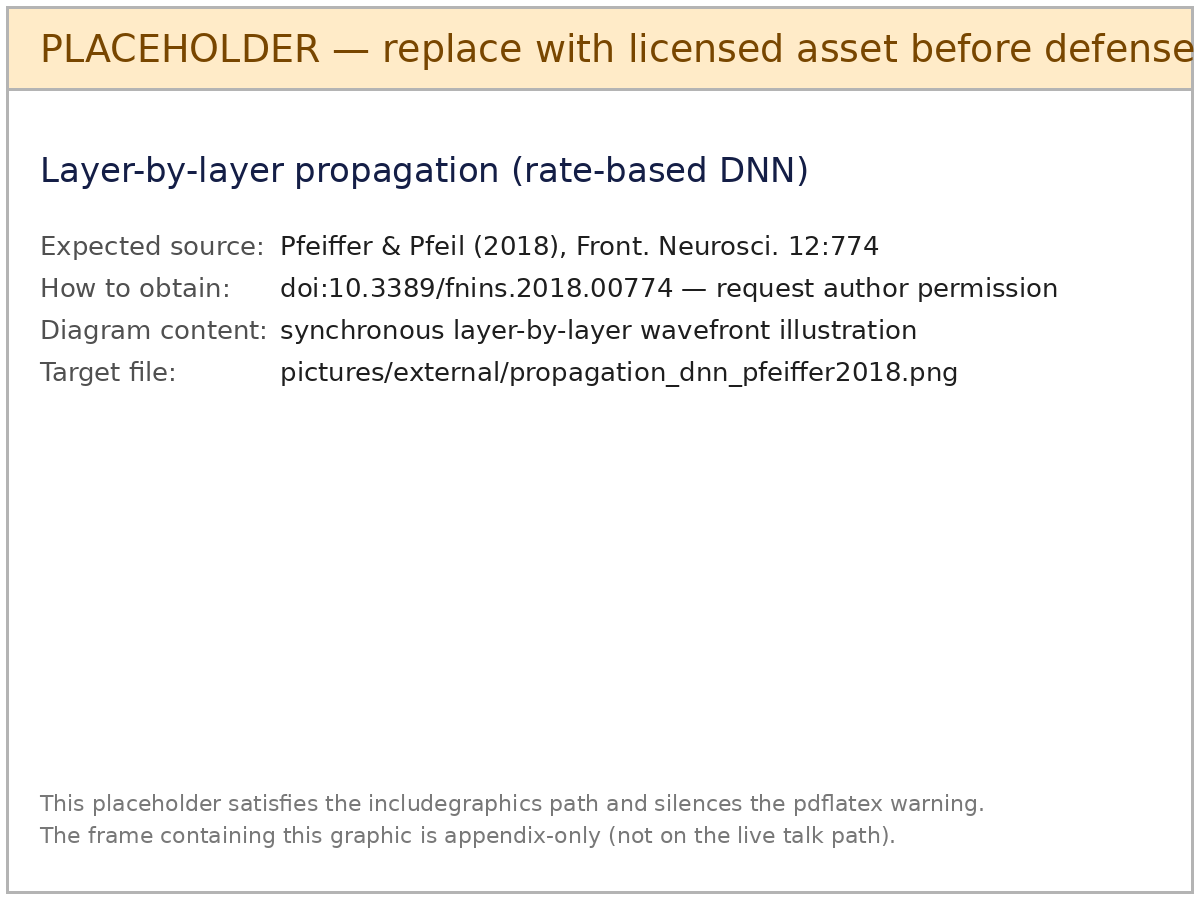
\includegraphics[width=0.92\textwidth]{pictures/external/propagation_dnn_pfeiffer2018.png}\\[1pt]
      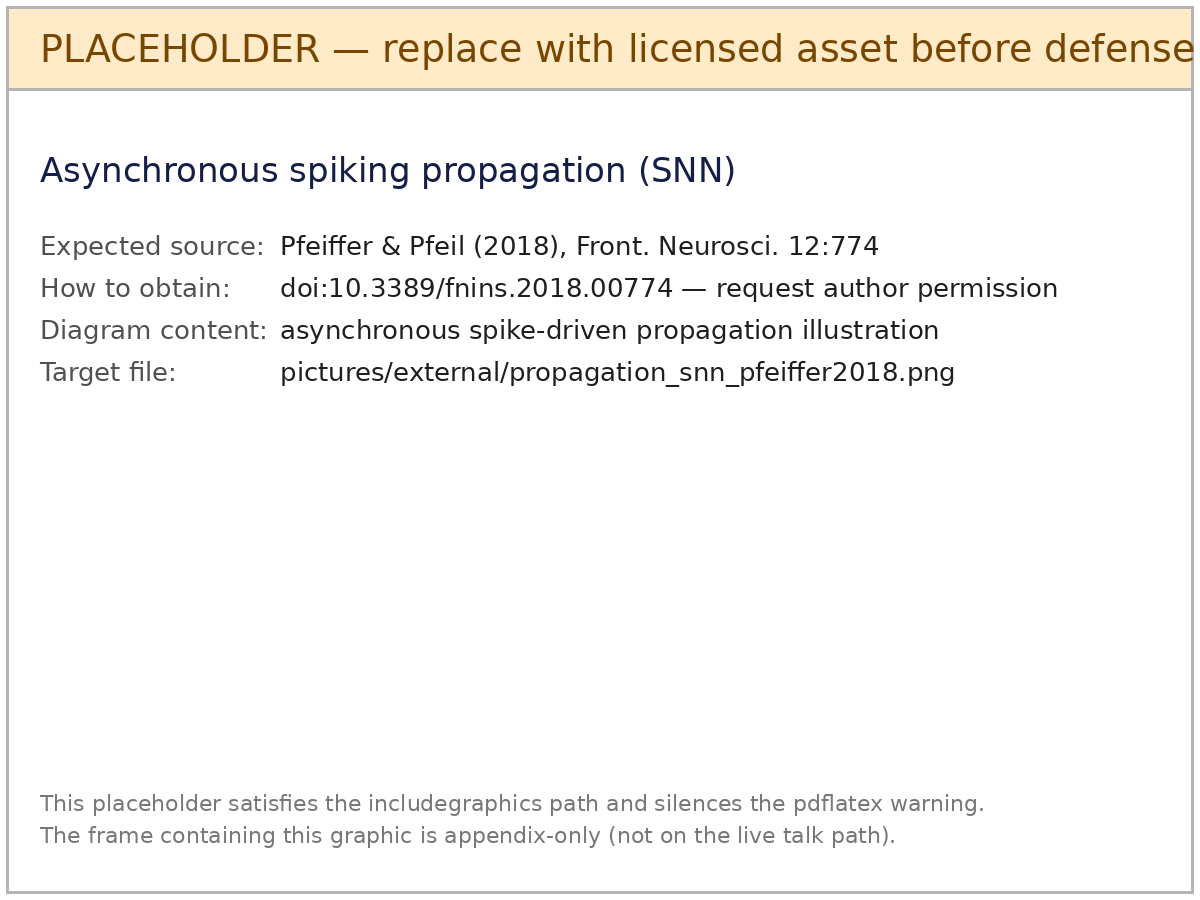
\includegraphics[width=0.92\textwidth]{pictures/external/propagation_snn_pfeiffer2018.png}\\
      \srccap{Layer-by-layer vs.\ asynchronous propagation (Pfeiffer \& Pfeil 2018)}
    \end{column}
  \end{columns}
\end{frame}

\begin{frame}{Appendix --- Why a linear readout suffices (Koopman lens)}
  For a nonlinear map $\mathbf{F}$, the Koopman operator acts linearly on
  observables by composition: $(\mathcal{K} g)(\mathbf{x}) = g(\mathbf{F}(\mathbf{x}))$.
  The spiking reservoir lifts the low-dimensional scalp signal into a
  high-dimensional space where the driven dynamics are more nearly
  linearizable on observables. A linear readout's success is the predicted
  outcome --- not an empirical convenience \refcite{Brunton et al.\ 2022}.
\end{frame}

\begin{frame}{Appendix --- LSM canonical schematic}
  \centering
  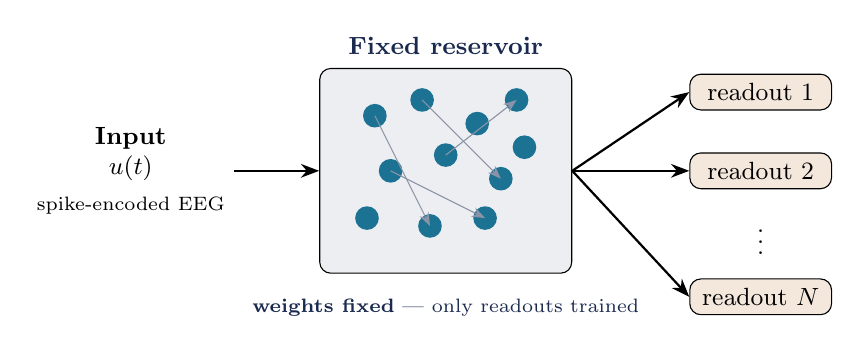
\begin{tikzpicture}[font=\small,>=Stealth]
    \node[align=center] (in) at (0,0) {\textbf{Input}\\$u(t)$\\[2pt]{\scriptsize spike-encoded EEG}};
    \node[draw,rounded corners,fill=sbnavy!8,minimum width=3.2cm,minimum height=2.6cm] (res) at (4.0,0) {};
    \node[above=0.5mm of res,sbnavy]{\textbf{Fixed reservoir}};
    \foreach \p in {(3.1,0.7),(3.7,0.9),(4.4,0.6),(4.9,0.9),(3.3,0.0),(4.0,0.2),(4.7,-0.1),(3.0,-0.6),(3.8,-0.7),(4.5,-0.6),(5.0,0.3)}
      \node[circle,fill=sbteal,minimum size=3mm,inner sep=0] at \p {};
    \draw[sbgrey,->](3.1,0.7)--(3.8,-0.7);
    \draw[sbgrey,->](3.7,0.9)--(4.7,-0.1);
    \draw[sbgrey,->](4.0,0.2)--(4.9,0.9);
    \draw[sbgrey,->](3.3,0.0)--(4.5,-0.6);
    \node[draw,rounded corners,fill=sbaccent!15,minimum width=1.8cm] (r1) at (8.0,1.0){readout $1$};
    \node[draw,rounded corners,fill=sbaccent!15,minimum width=1.8cm] (r2) at (8.0,0.0){readout $2$};
    \node[align=center] at (8.0,-0.8){$\vdots$};
    \node[draw,rounded corners,fill=sbaccent!15,minimum width=1.8cm] (rN) at (8.0,-1.6){readout $N$};
    \draw[->,thick](in.east)--(res.west);
    \draw[->,thick](res.east)--(r1.west);
    \draw[->,thick](res.east)--(r2.west);
    \draw[->,thick](res.east)--(rN.west);
    \node[below=2mm of res,align=center,font=\scriptsize,sbnavy]{\textbf{weights fixed} --- only readouts trained};
  \end{tikzpicture}
\end{frame}

\begin{frame}{Appendix --- The interpretable-EEG landscape}
  \begin{itemize}\small
    \item \textbf{Post-hoc attribution.} SHAP, attention rollout, saliency on
      EEGNet; SNN-specific Spike Activation Map
      \refcite{Kim \& Panda 2021}, SNN attention \refcite{Yao et al.\ 2023}.
      Explain what the model attended to.
    \item \textbf{Brain-structured SNNs.} NeuCube \refcite{Kasabov 2014}:
      atlas-structured reservoir; clusters align with ERP stages
      \refcite{Doborjeh et al.\ 2021}.
    \item \textbf{Prototype reasoning.} ProtoPMed-EEG
      \refcite{Barnett et al.\ 2024}: clinician-validated; prototype
      explanation raised reader accuracy on ICU EEG from $47\%$ to $71\%$.
    \item \textbf{High-accuracy black boxes.} EEGNet
      \refcite{Lawhern et al.\ 2018}: top accuracy, post-hoc explanation only.
  \end{itemize}
\end{frame}

\begin{frame}{Appendix --- Why a fixed reservoir over a trained deep SNN}
  \begin{itemize}\small
    \item End-to-end deep SNNs require backpropagation-through-time with
      surrogate gradients; forward/backward mismatch destabilizes long-horizon
      learning \refcite{Neftci et al.\ 2019}.
    \item A fixed reservoir bypasses temporal credit assignment entirely.
    \item Untrained dynamics are analyzable as a driven nonlinear system ---
      the interpretability contribution weight adaptation would obscure.
    \item GNNs on conventional features (band power, differential entropy)
      represent the signal as a static spatial snapshot
      \refcite{Jia et al.\ 2024} --- discarding the transient dynamics a
      reservoir preserves.
  \end{itemize}
\end{frame}

\begin{frame}{Appendix --- Complete baseline table}
  \centering\small
  \begin{tabular}{lccc}\toprule
    Model & Uncentered & Centered & $\Delta$ \\\midrule
    EEGNet              & 72.0 & 89.1 & $+17.1$ \\
    Raw EEG + linear    & 70.5 & 88.4 & $+17.9$ \\
    PCA-200             & 64.9 & 86.4 & $+21.5$ \\
    GRU                 & 59.9 & 78.4 & $+18.5$ \\
    ARSPI-Net reservoir & 59.4 & 78.8 & $+19.4$ \\
    LSTM                & 58.0 & 71.1 & $+13.1$ \\
    Band power          & 47.7 & 61.0 & $+13.3$ \\
    \bottomrule
  \end{tabular}
  \vspace{0.6em}

  \normalsize {\small Centering moves every model $+13$ to $+22$\,pp.
  Architecture choice is secondary to the geometric correction. EEGNet,
  GRU, LSTM values triple-confirmed against stored results pickle.}
\end{frame}

\begin{frame}{Appendix --- Transform-fit provenance ($\Delta = 0$)}
  \begin{itemize}\small
    \item Test splits provably subject-disjoint; scaling fit on training folds
      only; no supervised selection.
    \item PCA was fit pooled pre-split in the reported path --- unsupervised
      and subject-disjoint, so no label or cross-subject leakage.
    \item \alert{Re-run with per-fold PCA refitting}: the centered headline
      path changes by $\Delta = 0.000$; the uncentered reservoir path
      \emph{improves} by $+3.3$\,pp. Subject-centering dominates fit scope.
  \end{itemize}
  \vspace{0.3em}
  {\small The pooled fit inflates no reported result; the correction is
  confirmed neutral-to-conservative.}
\end{frame}

\begin{frame}{Appendix --- GNN comparison detail}
  \centering
  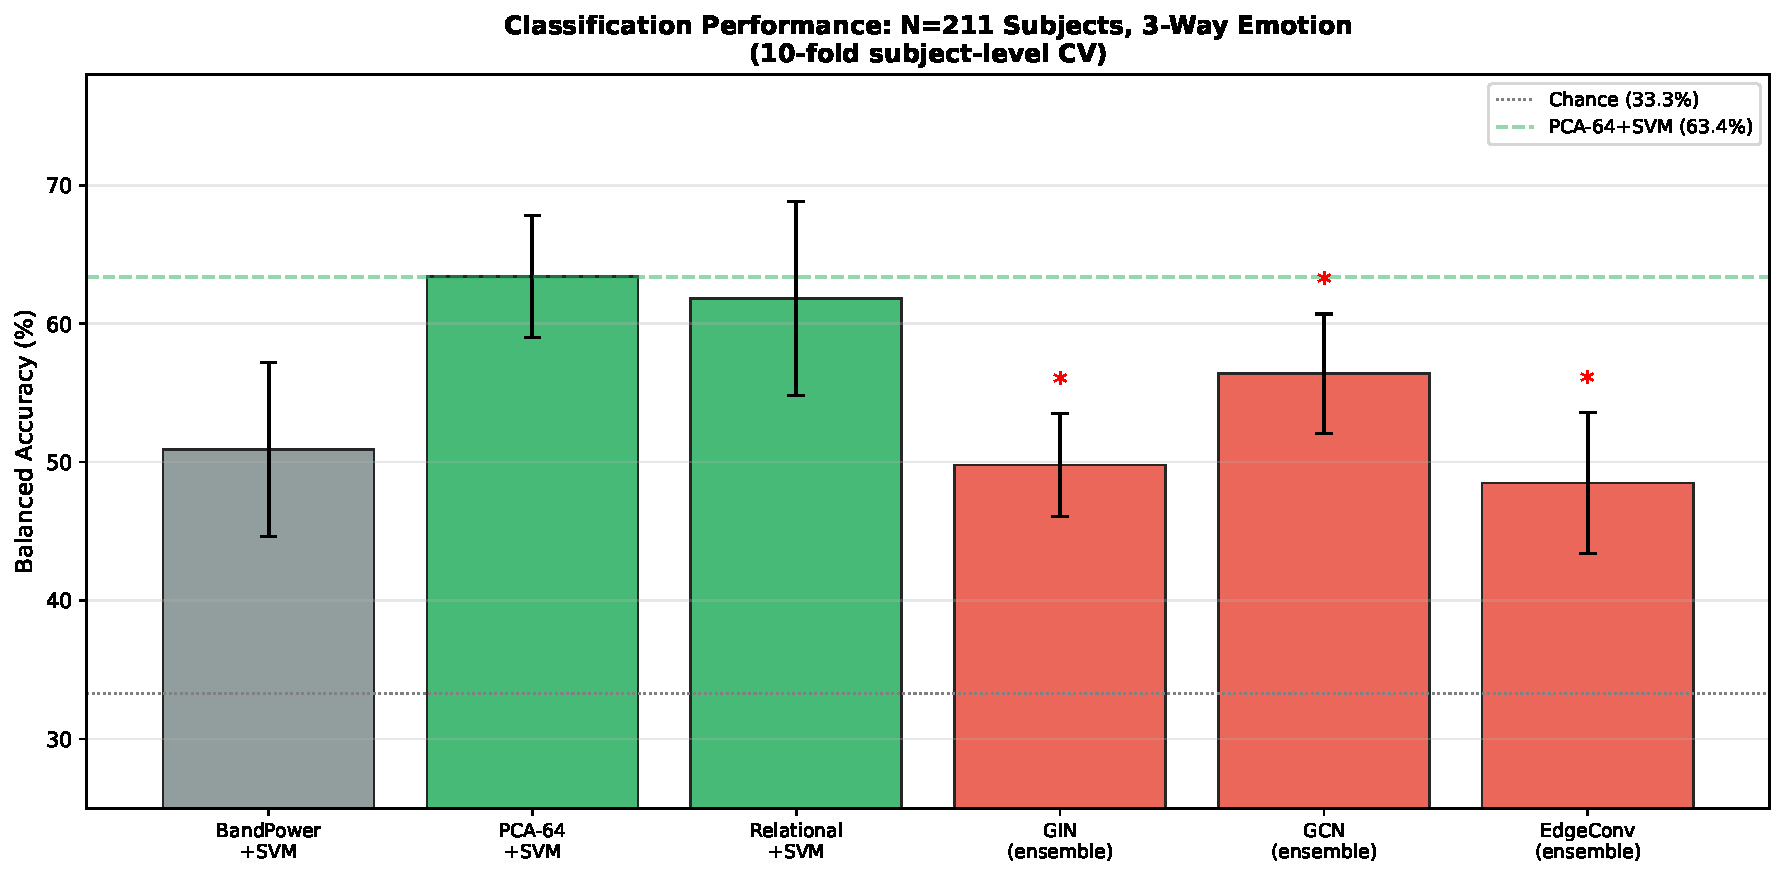
\includegraphics[height=0.78\textheight]{pictures/chGraphNeuralNetworks/fig_05_gnn_comparison_211.pdf}\\
  \srccap{Message-passing variants vs.\ concatenated embedding, $N=211$}
\end{frame}

\begin{frame}{Appendix --- Confusion matrix}
  \centering
  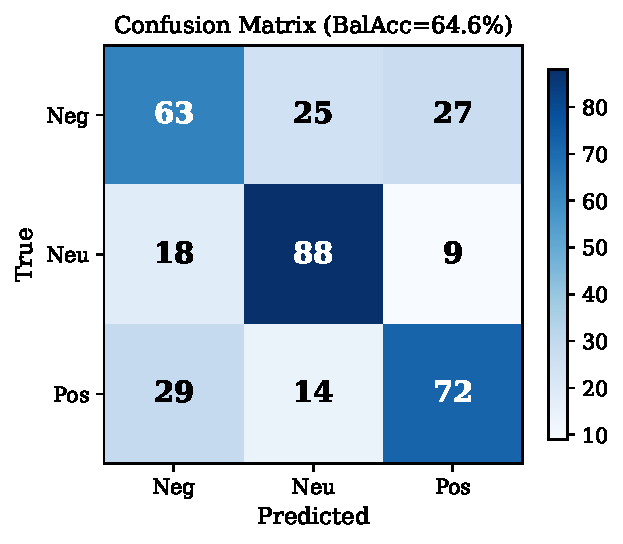
\includegraphics[height=0.78\textheight]{pictures/chGraphNeuralNetworks/confusion_matrix_best.pdf}
\end{frame}

\begin{frame}{Appendix --- ERP-window dependence}
  \centering
  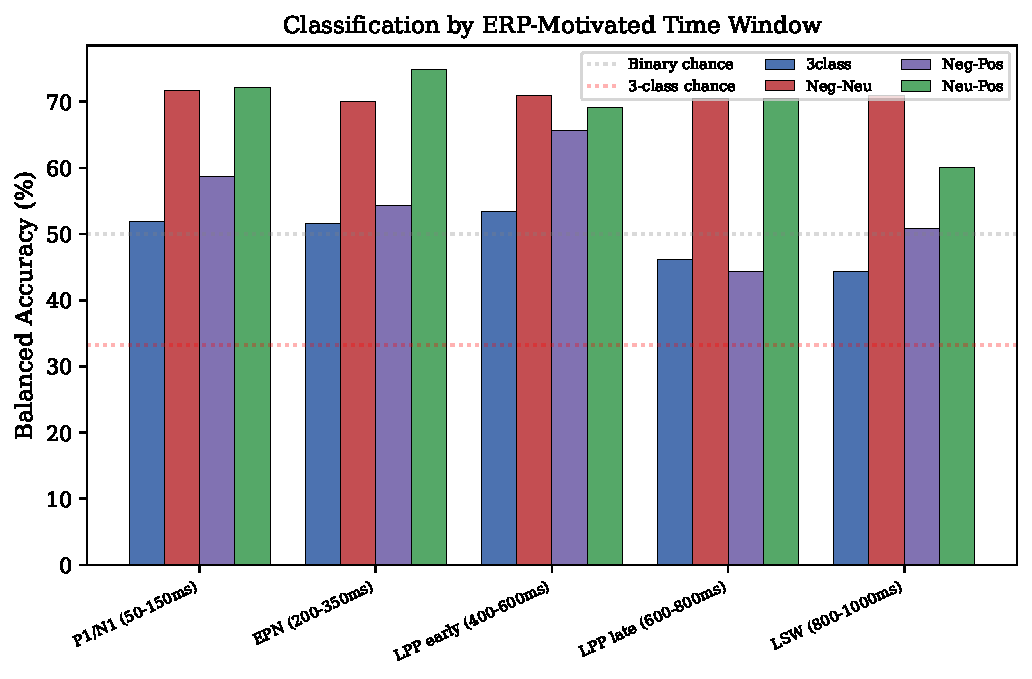
\includegraphics[height=0.78\textheight]{pictures/chDynamics/erp_window_comparison.pdf}
\end{frame}

\begin{frame}{Appendix --- Dissociation analysis}
  \centering
  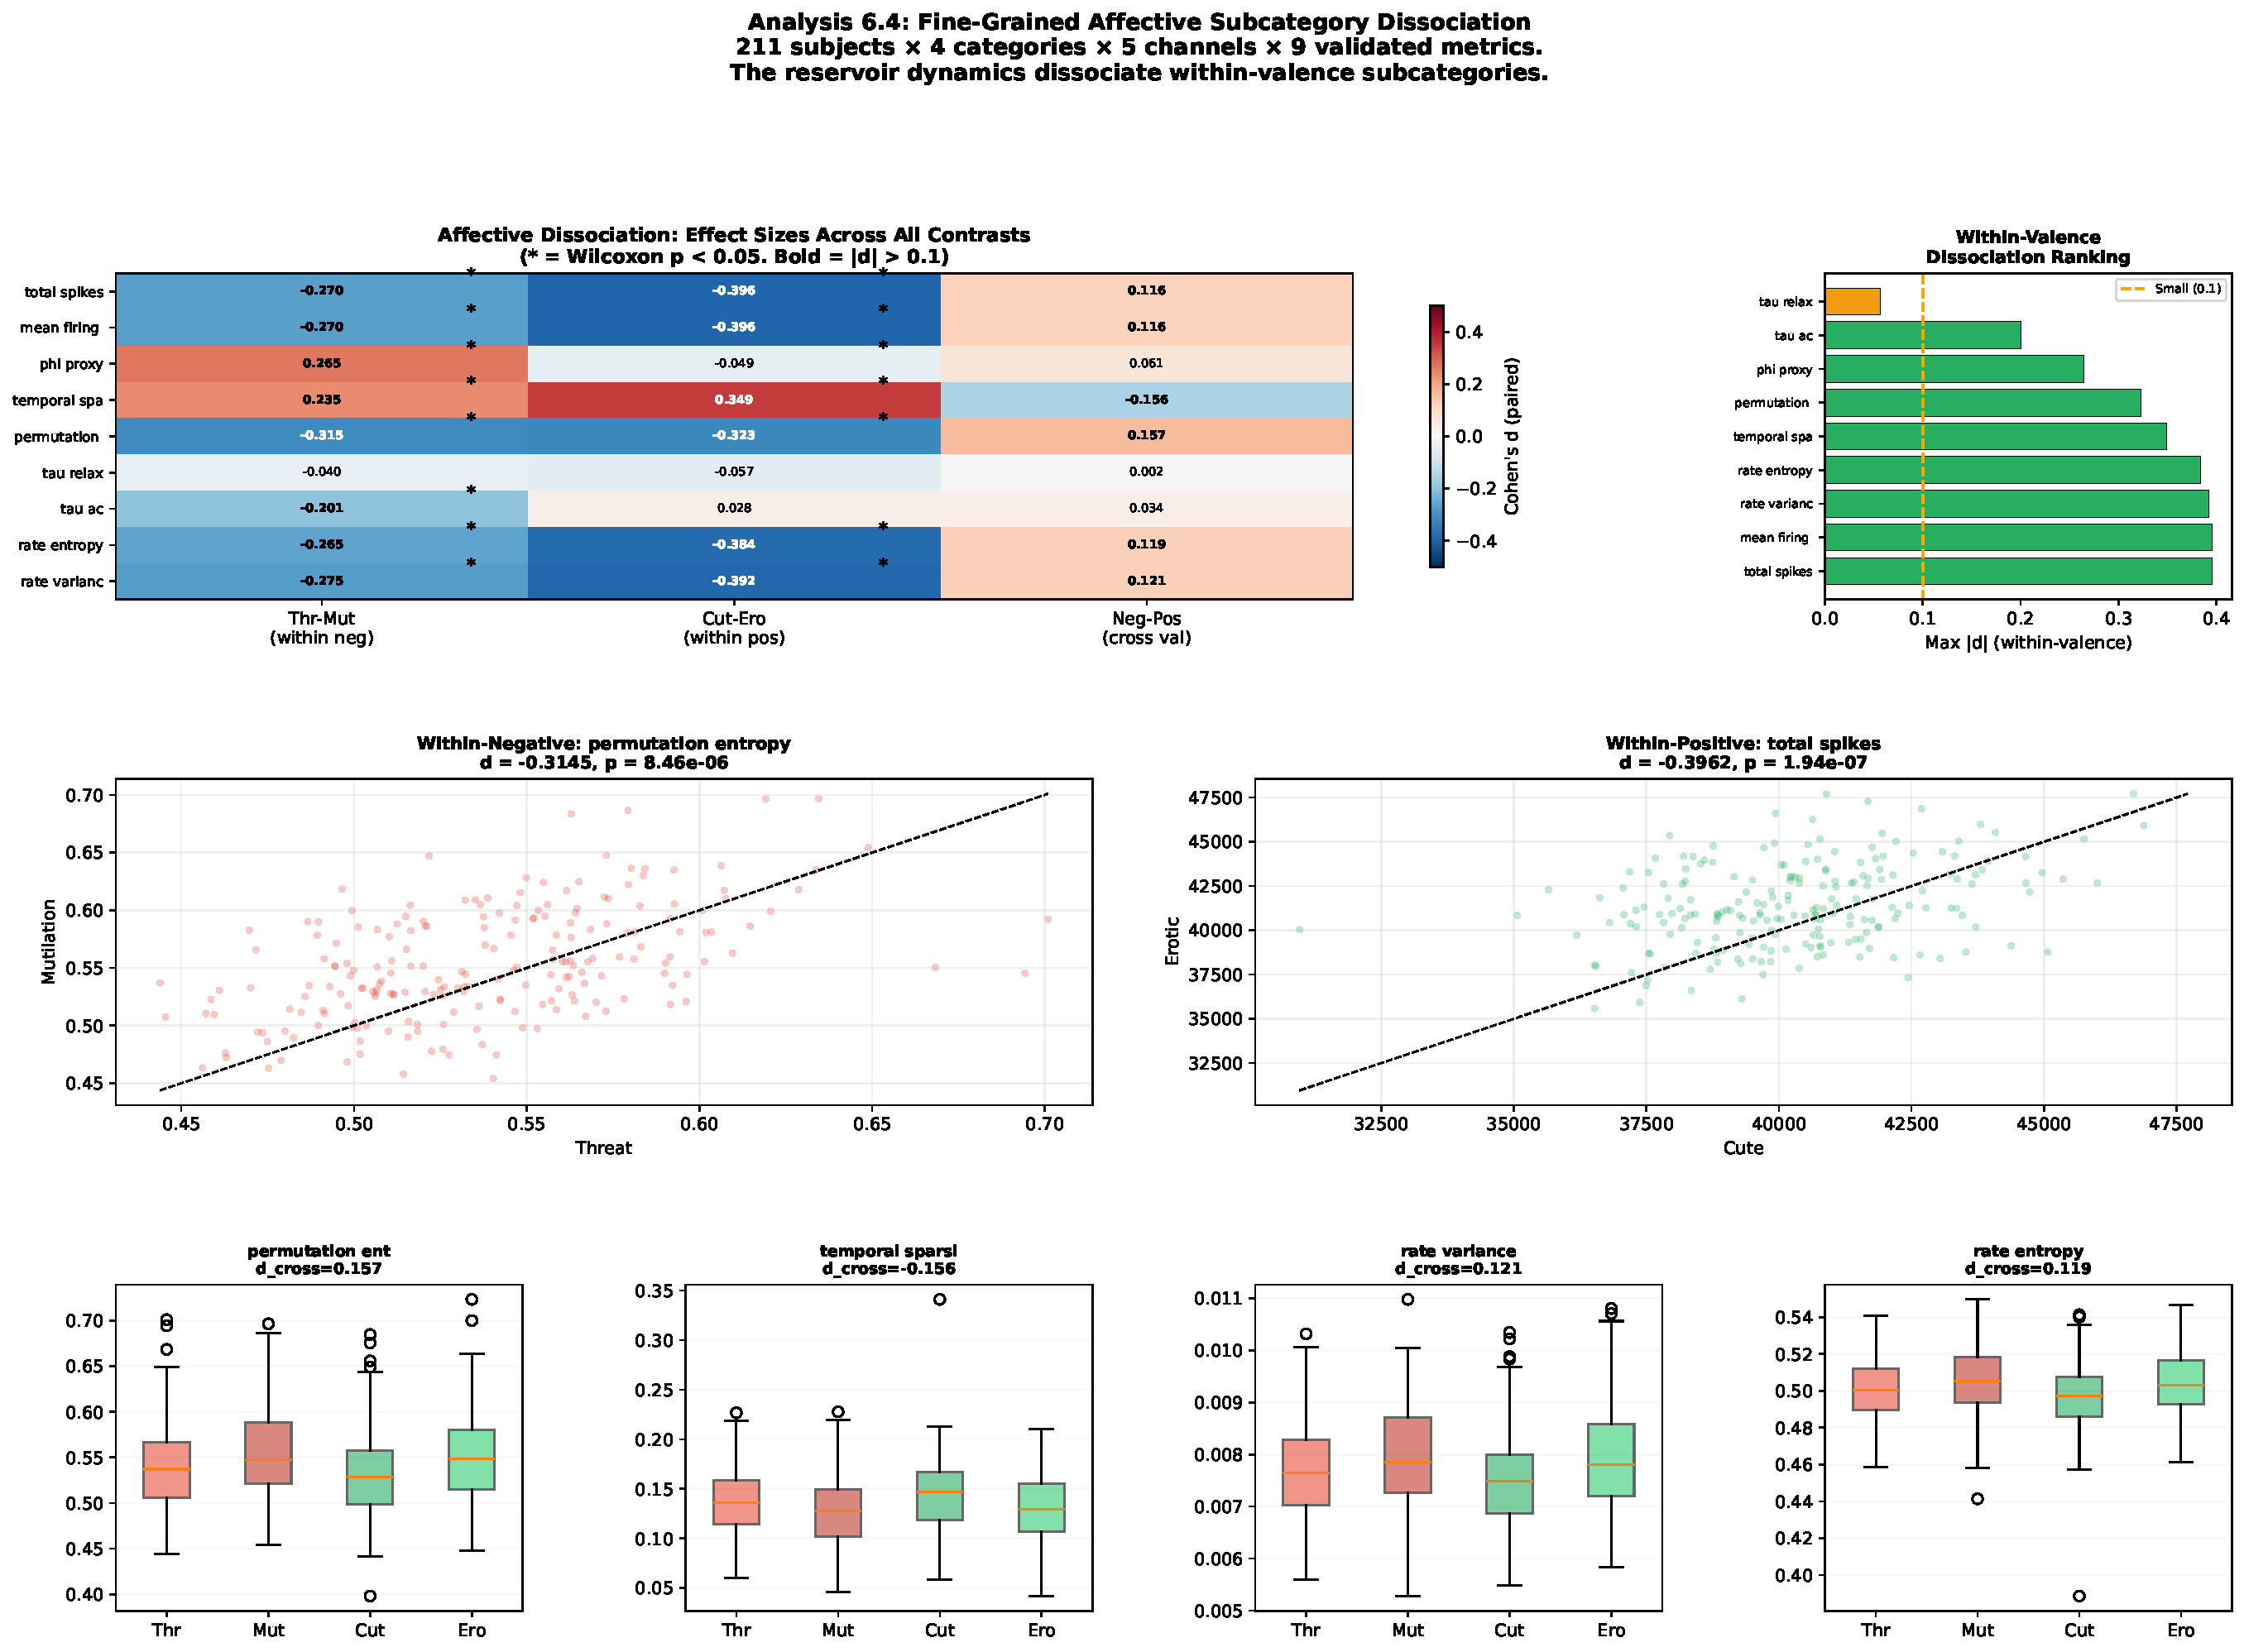
\includegraphics[height=0.78\textheight]{pictures/chDynamics/analysis6_4f_dissociation.pdf}
\end{frame}

\begin{frame}{Appendix --- HC vs.\ MDD contrast}
  \centering
  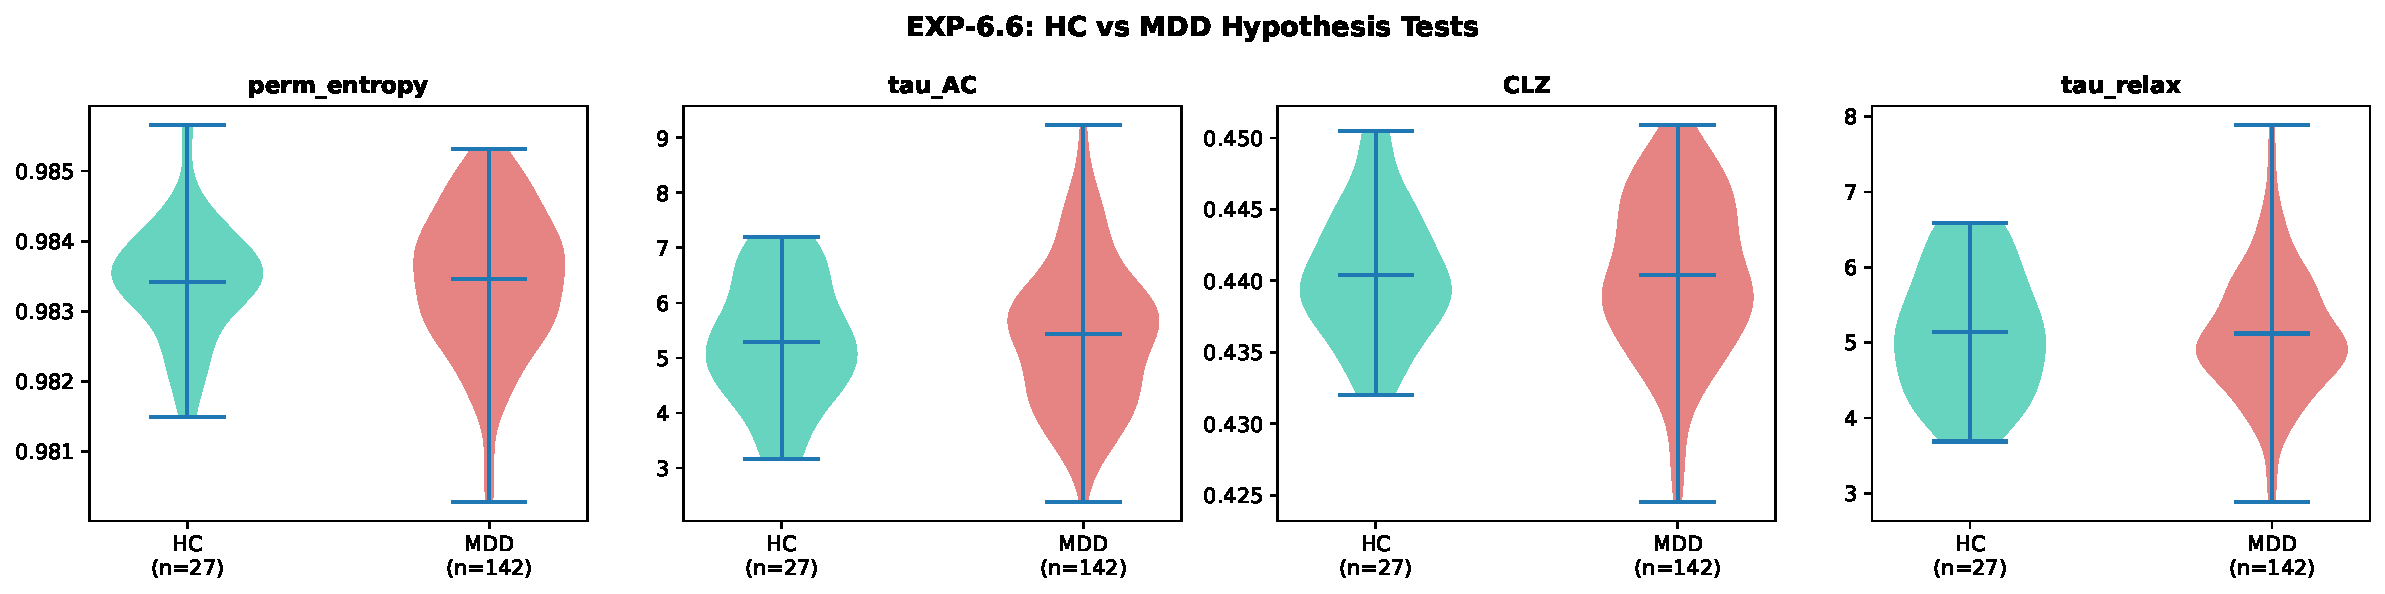
\includegraphics[height=0.78\textheight]{pictures/chDynamics/fig06_hc_vs_mdd.pdf}
\end{frame}

\begin{frame}{Appendix --- Layer-specific clinical sensitivity}
  \centering
  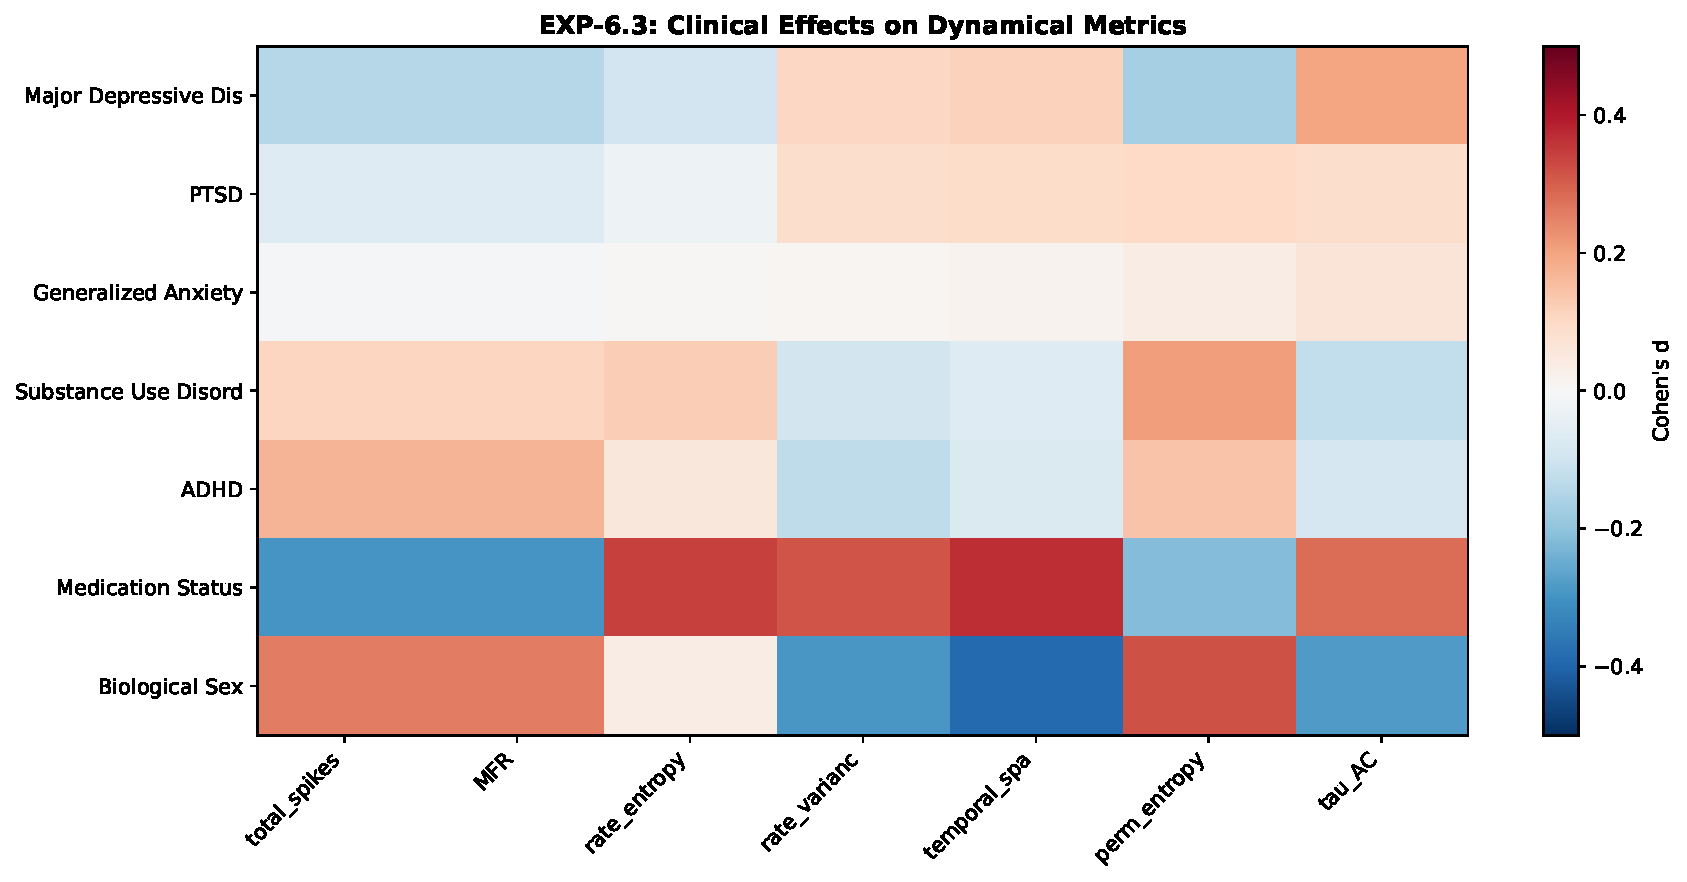
\includegraphics[height=0.78\textheight]{pictures/chDynamics/fig03_clinical_heatmap.pdf}
\end{frame}

\begin{frame}{Appendix --- Sparse coding analysis}
  \centering
  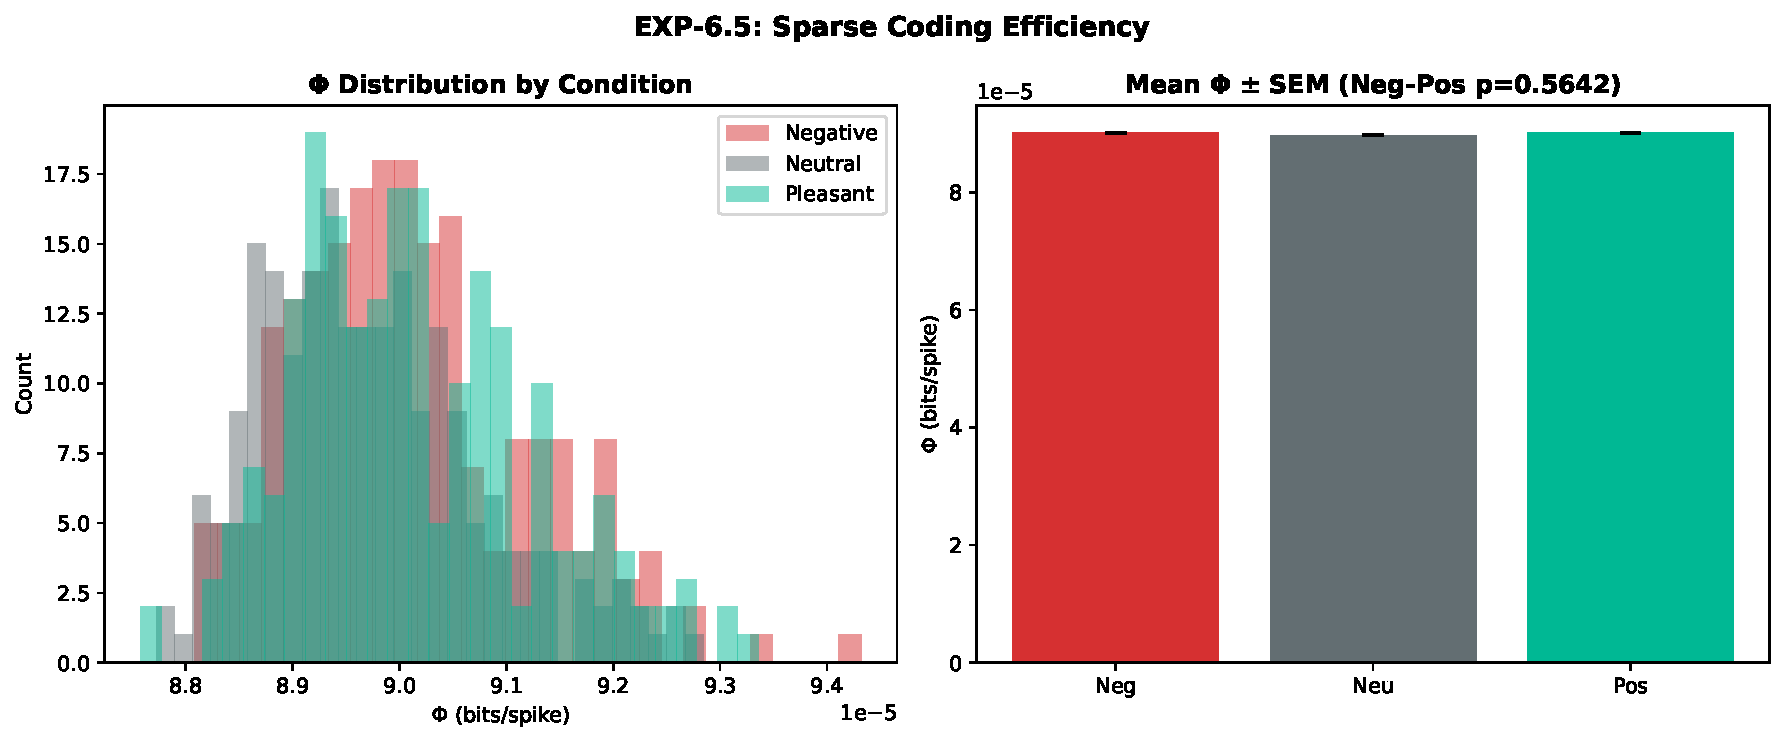
\includegraphics[height=0.78\textheight]{pictures/chDynamics/fig05_sparse_coding.pdf}
\end{frame}

\begin{frame}{Appendix --- $\Phi$ vs.\ $\tau$ by condition}
  \centering
  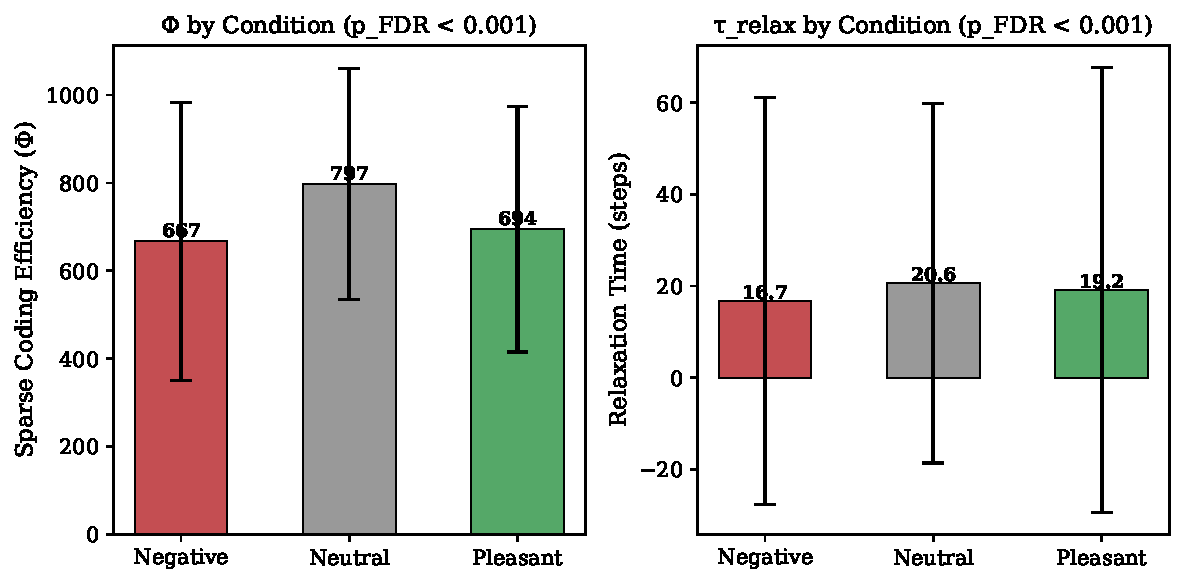
\includegraphics[height=0.78\textheight]{pictures/chDynamics/condition_phi_tau.pdf}
\end{frame}

\begin{frame}{Appendix --- Early vs.\ late $\Phi$}
  \centering
  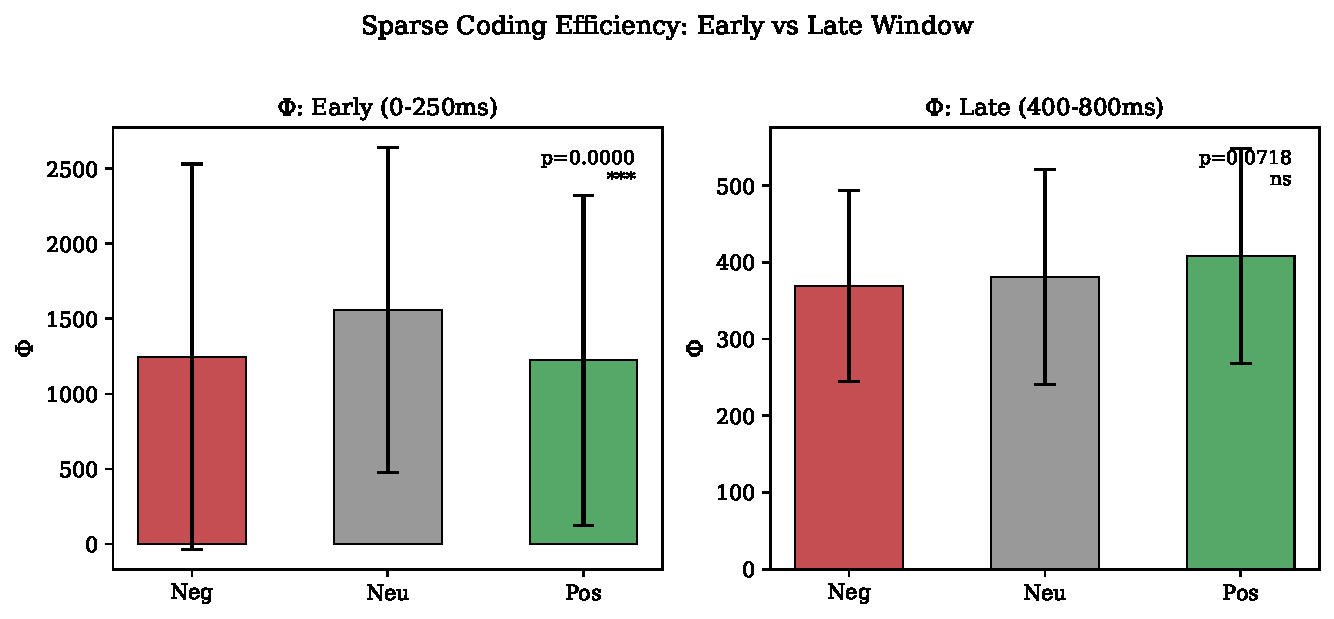
\includegraphics[height=0.78\textheight]{pictures/chDynamics/early_vs_late_phi.pdf}
\end{frame}

\begin{frame}{Appendix --- Classification under dynamics path}
  \centering
  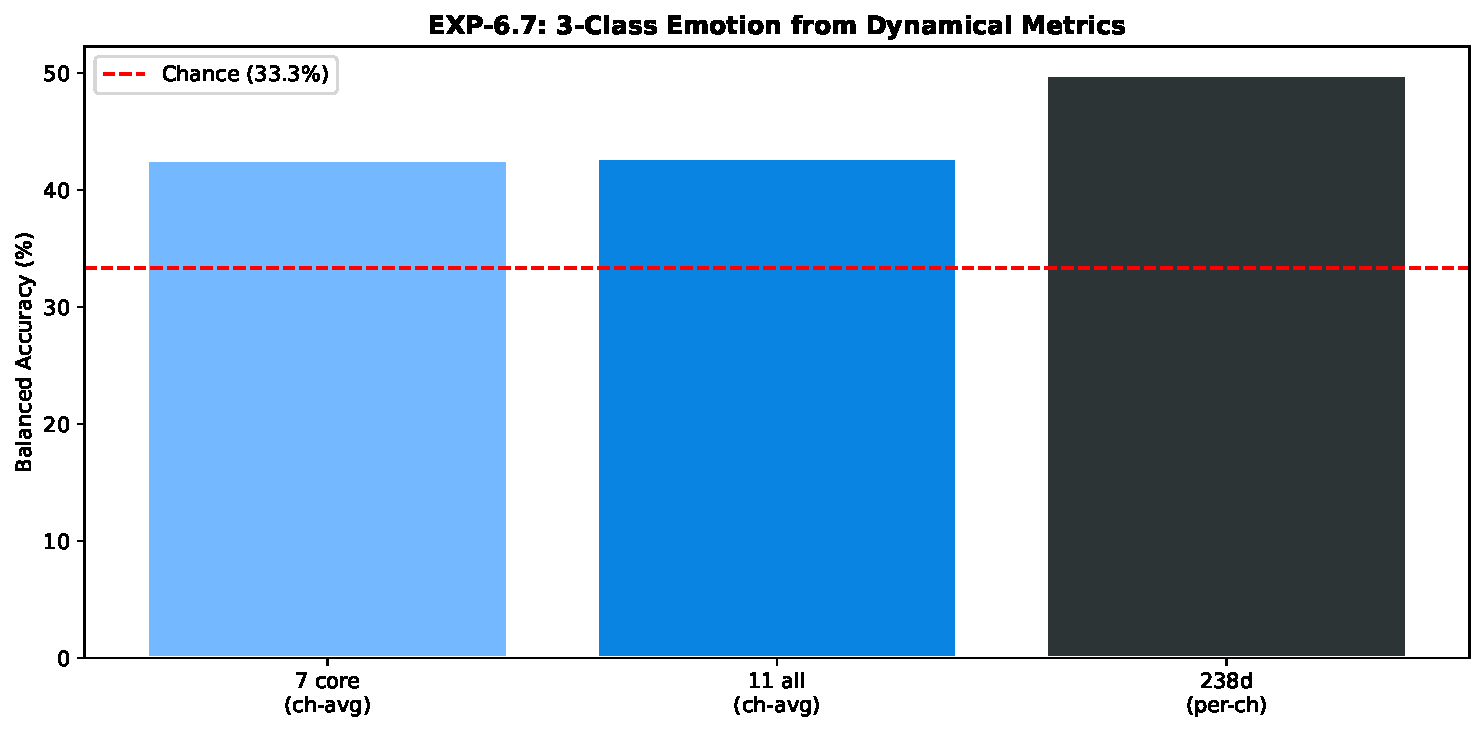
\includegraphics[height=0.78\textheight]{pictures/chDynamics/fig07_classification.pdf}
\end{frame}

\begin{frame}{Appendix --- Interaction analysis}
  \centering
  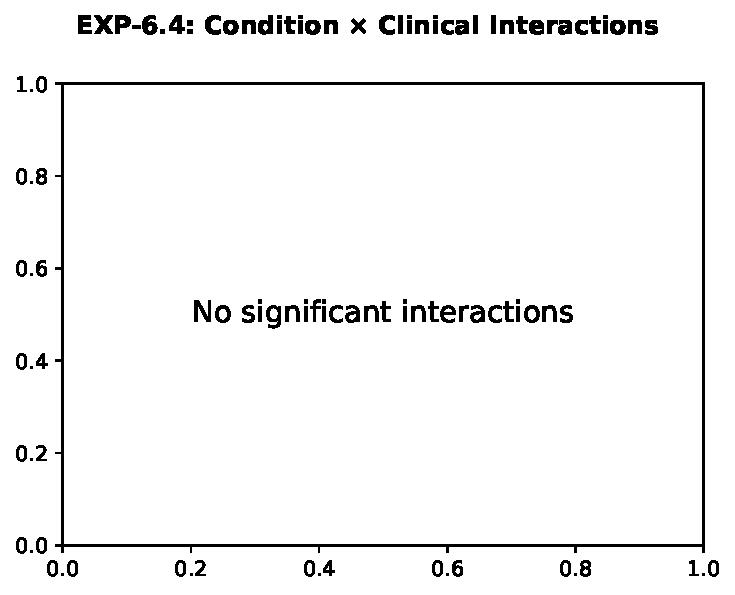
\includegraphics[height=0.78\textheight]{pictures/chDynamics/fig04_interactions.pdf}
\end{frame}

\begin{frame}{Appendix --- Mean coupling structure}
  \centering
  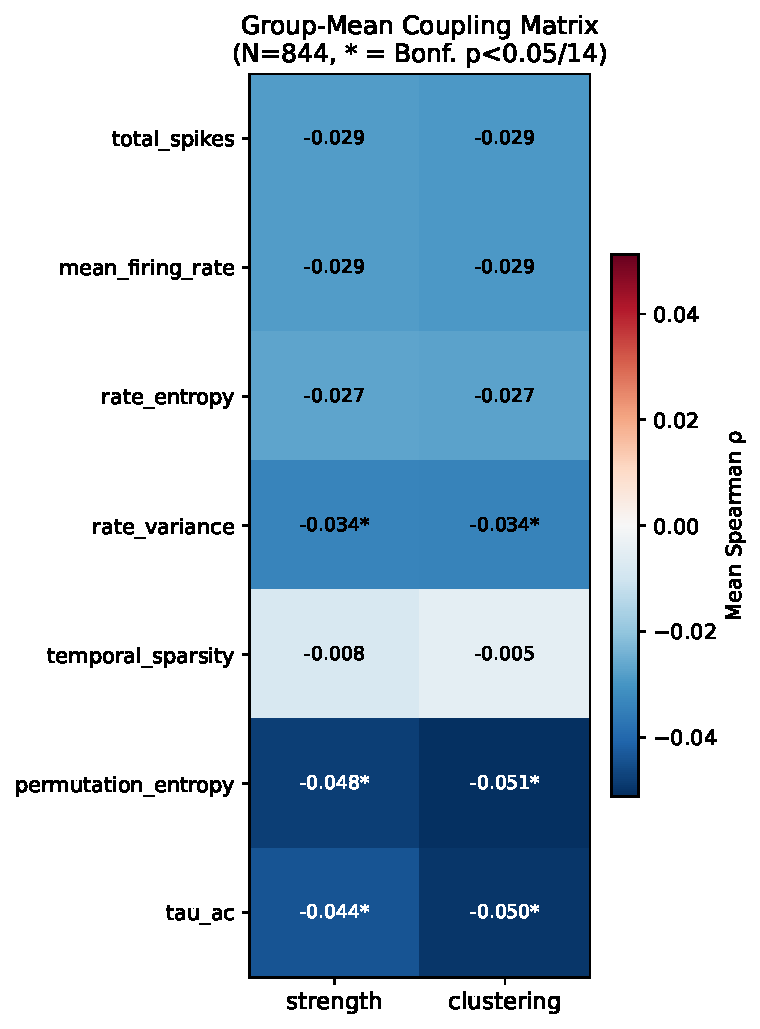
\includegraphics[height=0.78\textheight]{pictures/chSynthesis/fig7_A1_mean_coupling_matrix.pdf}
\end{frame}

\begin{frame}{Appendix --- $\kappa$ by affective category}
  \centering
  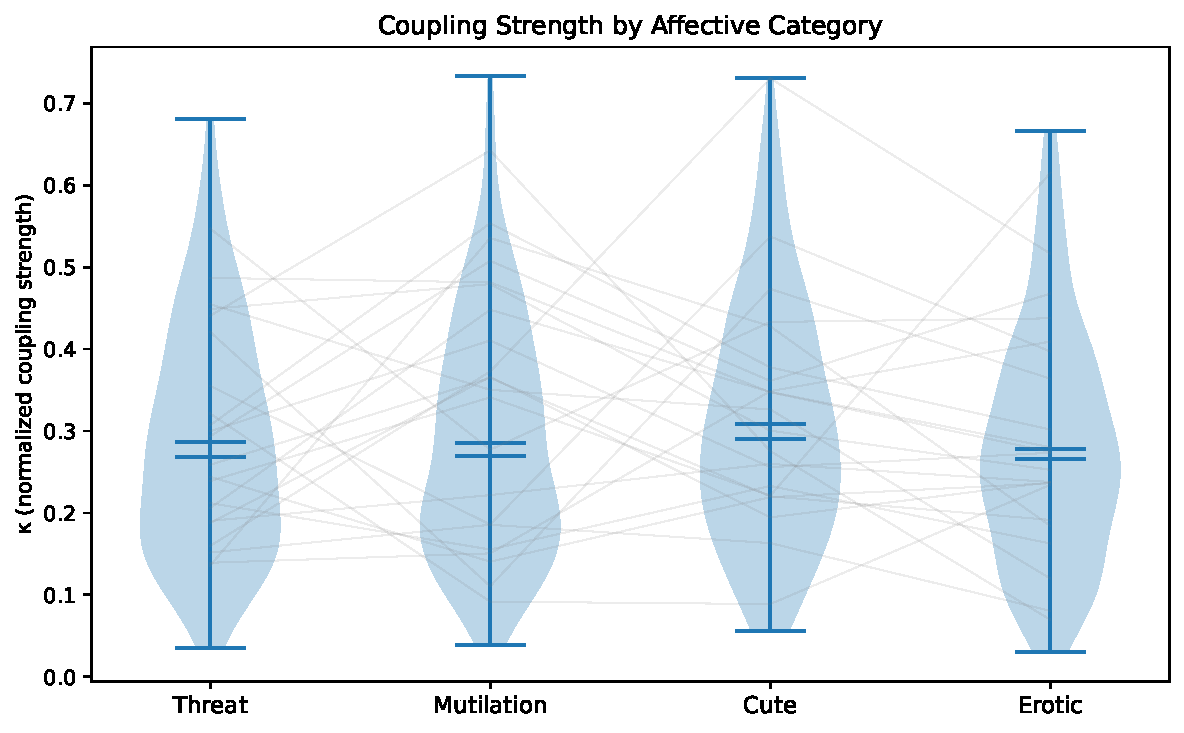
\includegraphics[height=0.78\textheight]{pictures/chSynthesis/fig7_A4_kappa_by_category.pdf}
\end{frame}

\begin{frame}{Appendix --- Diagnosis-associated coupling}
  \centering
  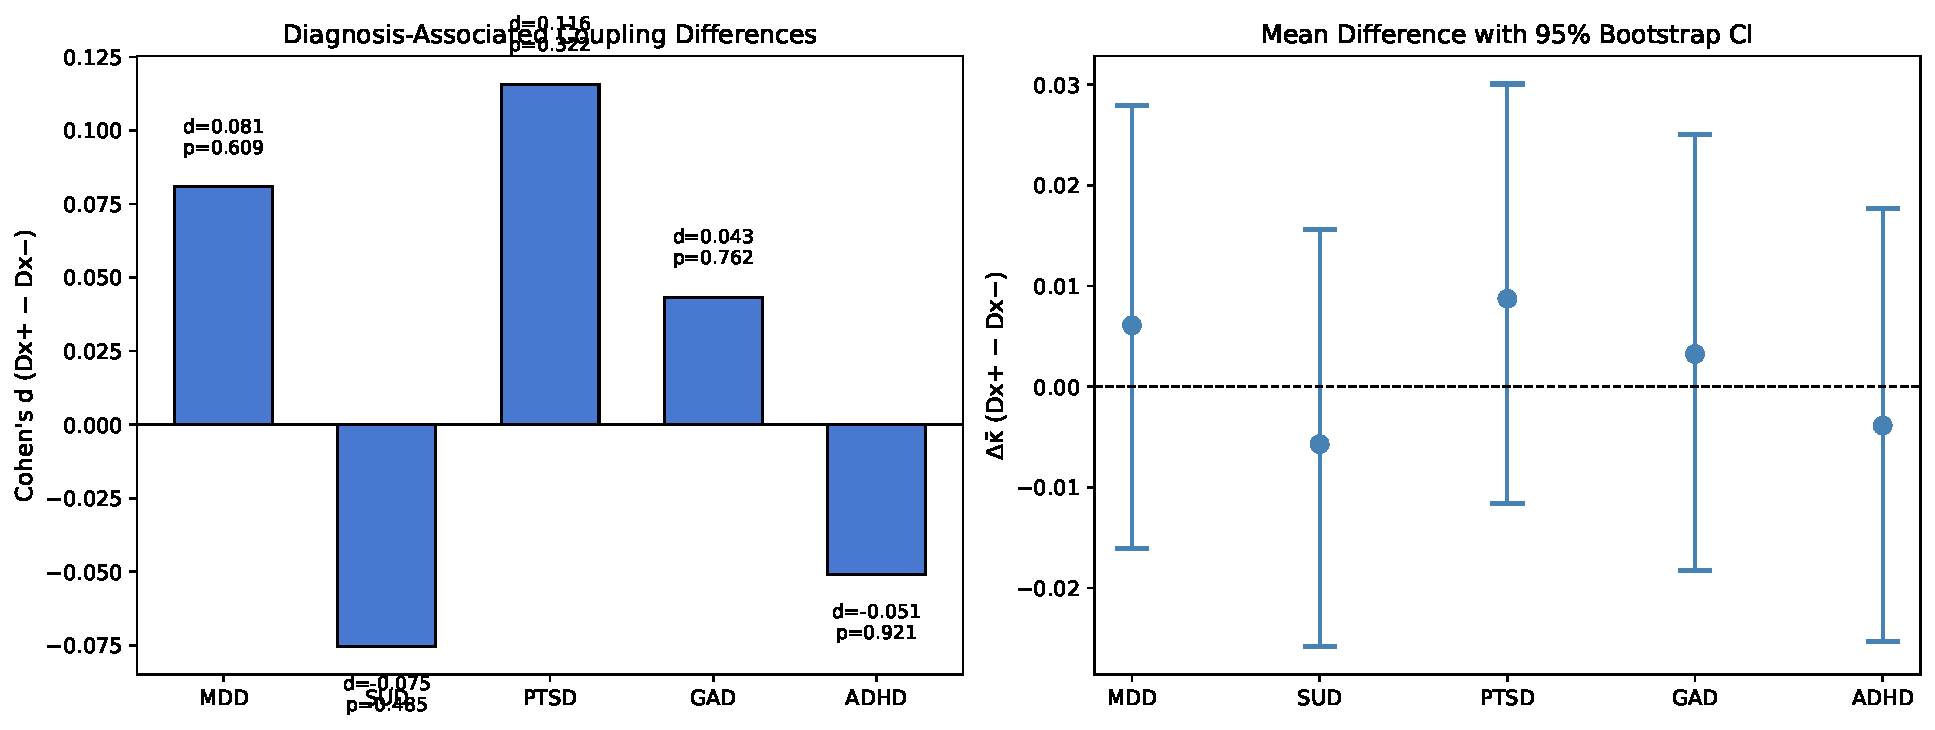
\includegraphics[height=0.78\textheight]{pictures/chSynthesis/fig7_D2_diagnosis_effects.pdf}
\end{frame}

\begin{frame}{Appendix --- Coupling-augmented classification}
  \centering
  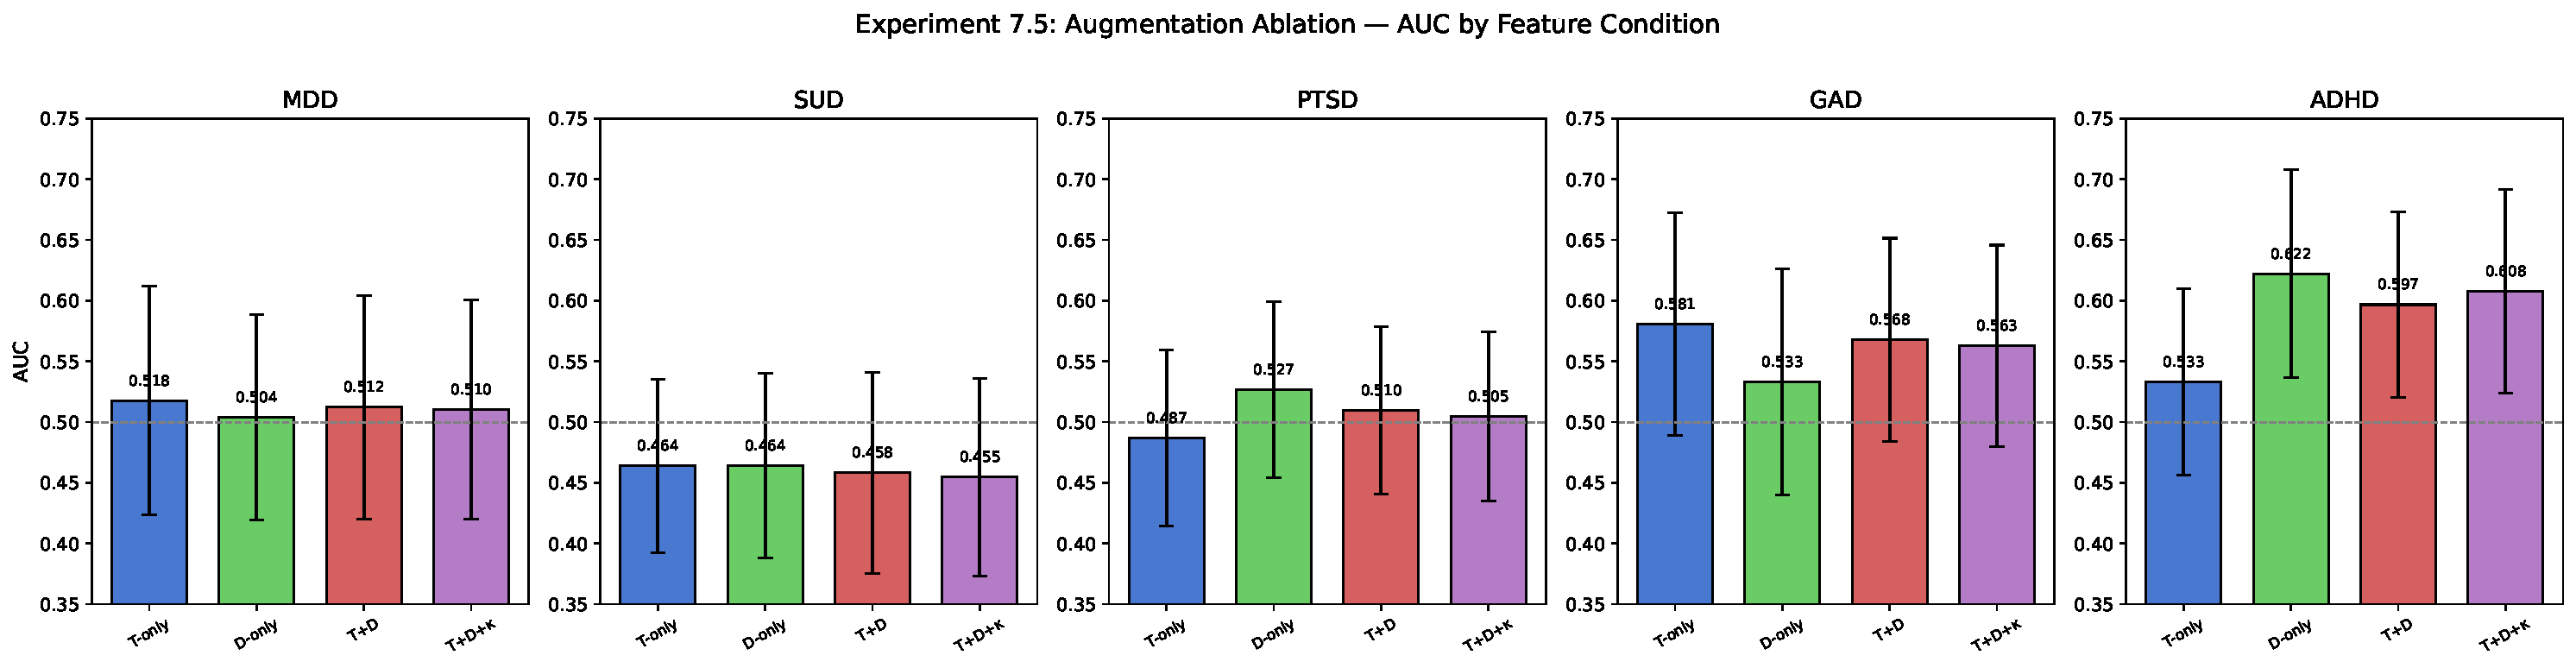
\includegraphics[height=0.78\textheight]{pictures/chSynthesis/fig7_E1_augmentation_auc.pdf}
\end{frame}

\begin{frame}{Appendix --- Category coupling matrices}
  \centering
  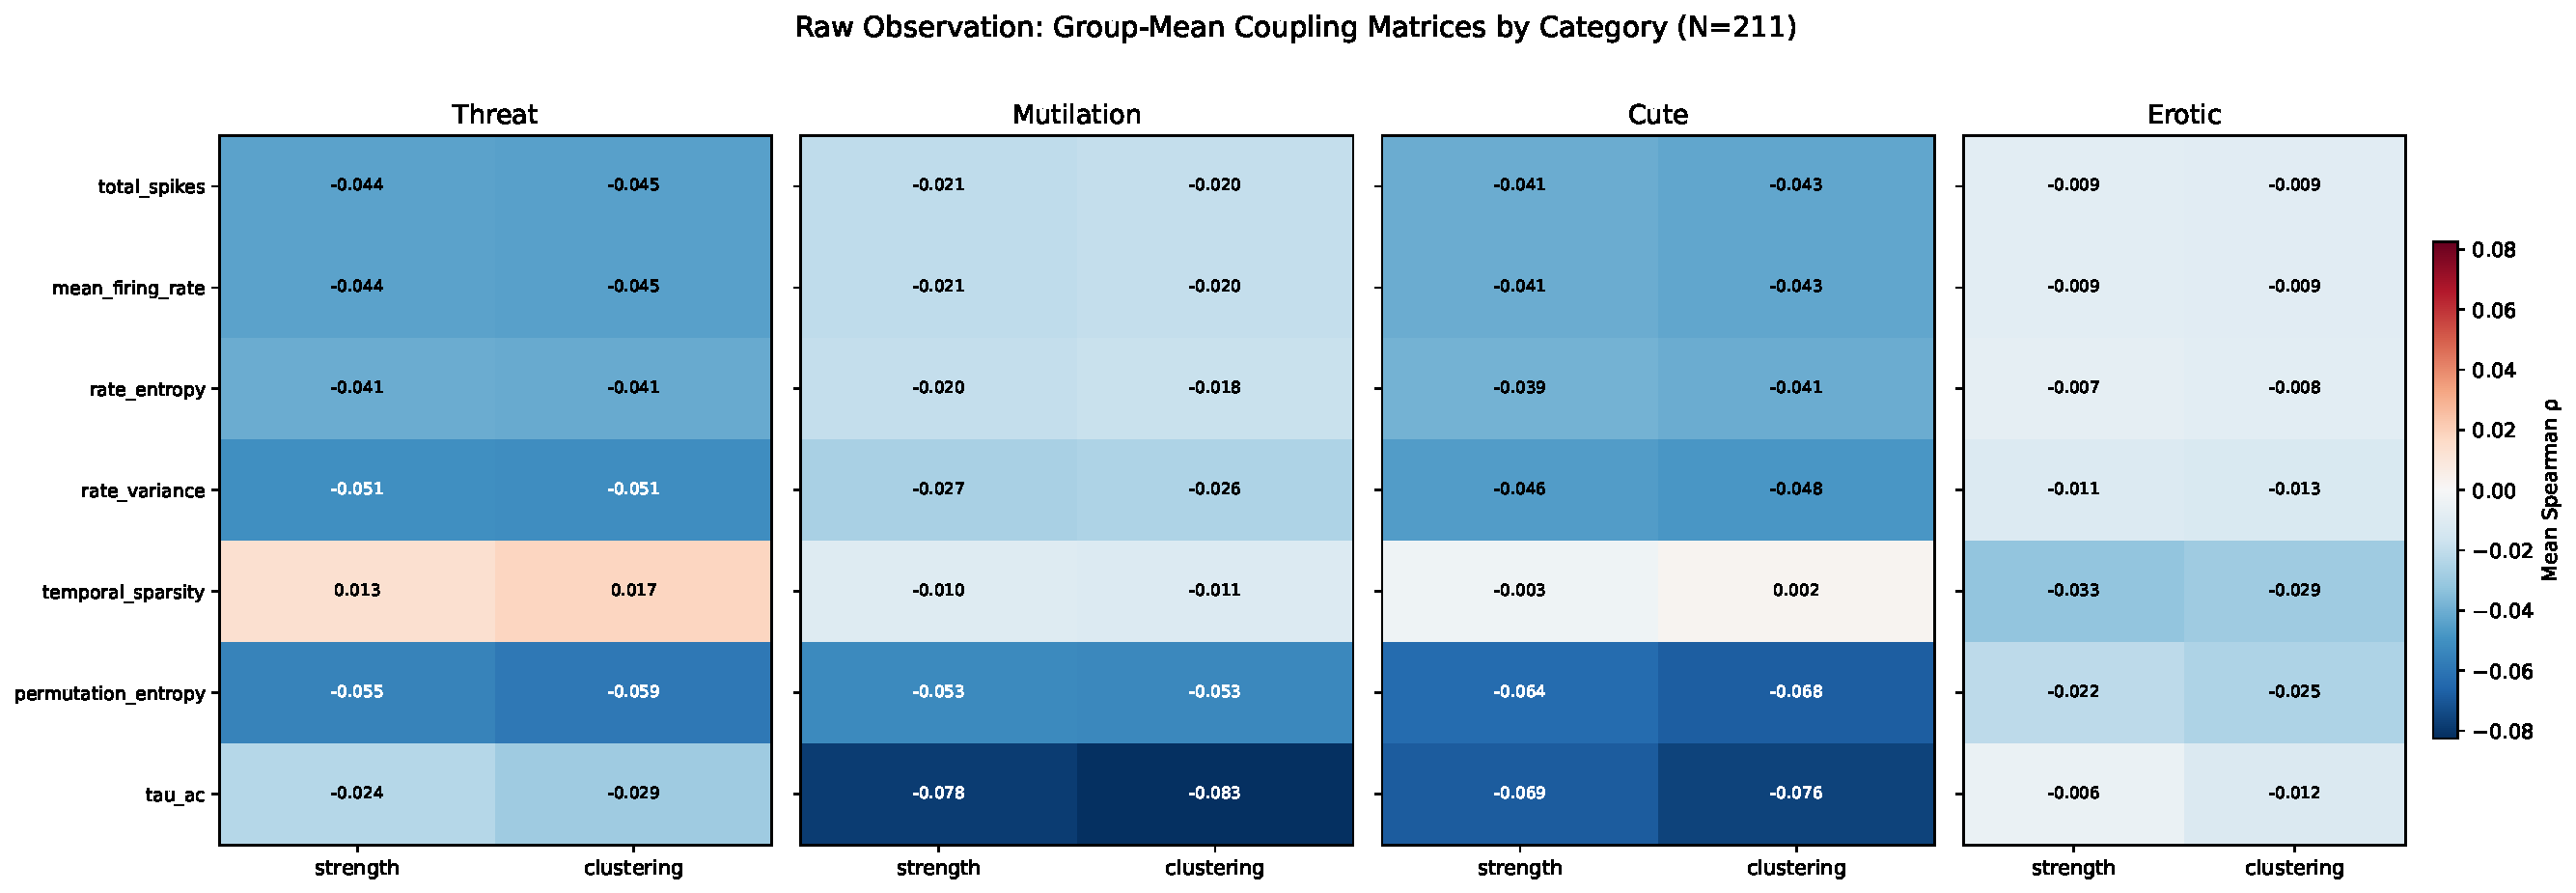
\includegraphics[height=0.78\textheight]{pictures/chSynthesis/fig7_C1_category_C_matrices.pdf}
\end{frame}

\begin{frame}{Appendix --- Coupling difference significance}
  \centering
  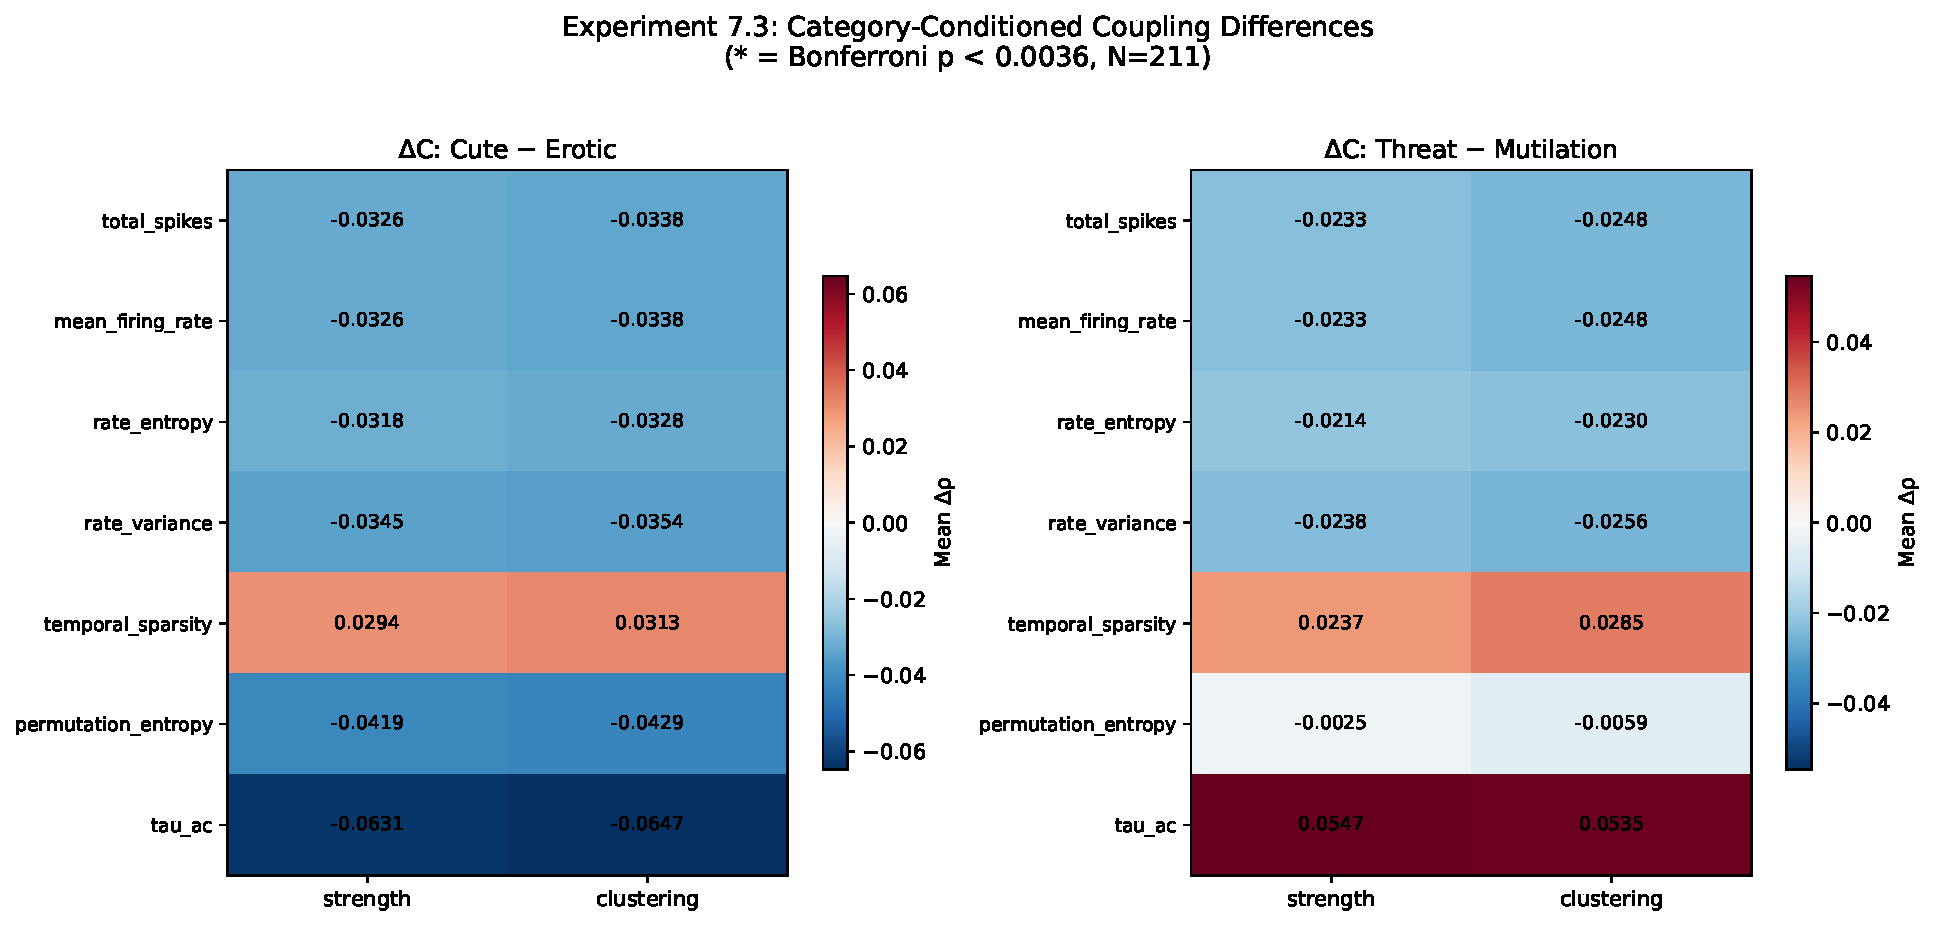
\includegraphics[height=0.78\textheight]{pictures/chSynthesis/fig7_C3_difference_significance.pdf}
\end{frame}

\begin{frame}{Appendix --- Variance decomposition (detail)}
  \centering
  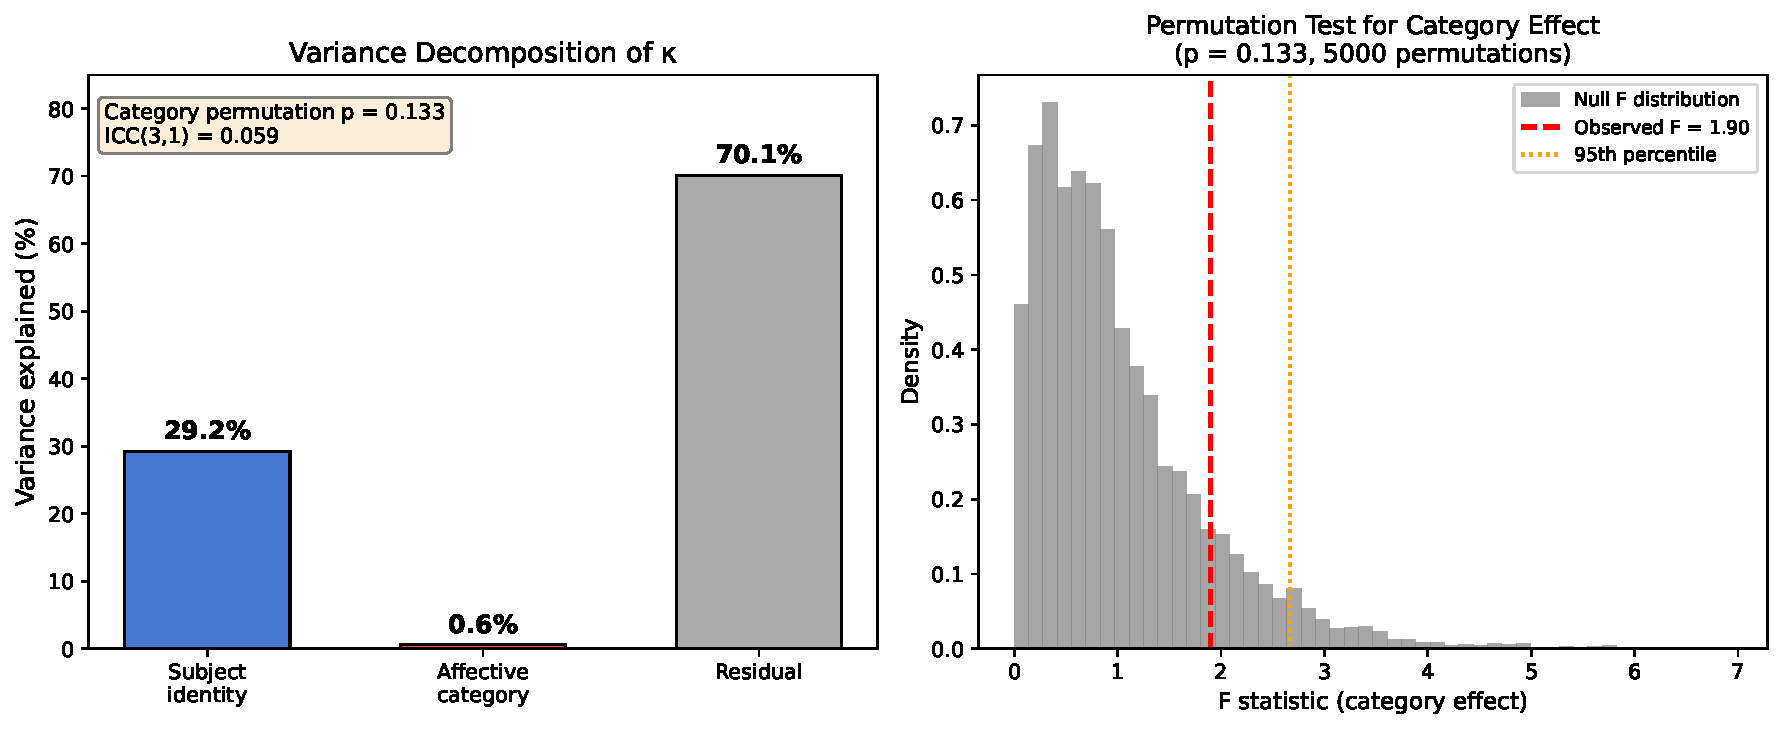
\includegraphics[height=0.78\textheight]{pictures/chSynthesis/fig7_B1_variance_decomposition.pdf}
\end{frame}

\begin{frame}{Appendix --- Defense summary figure}
  \centering
  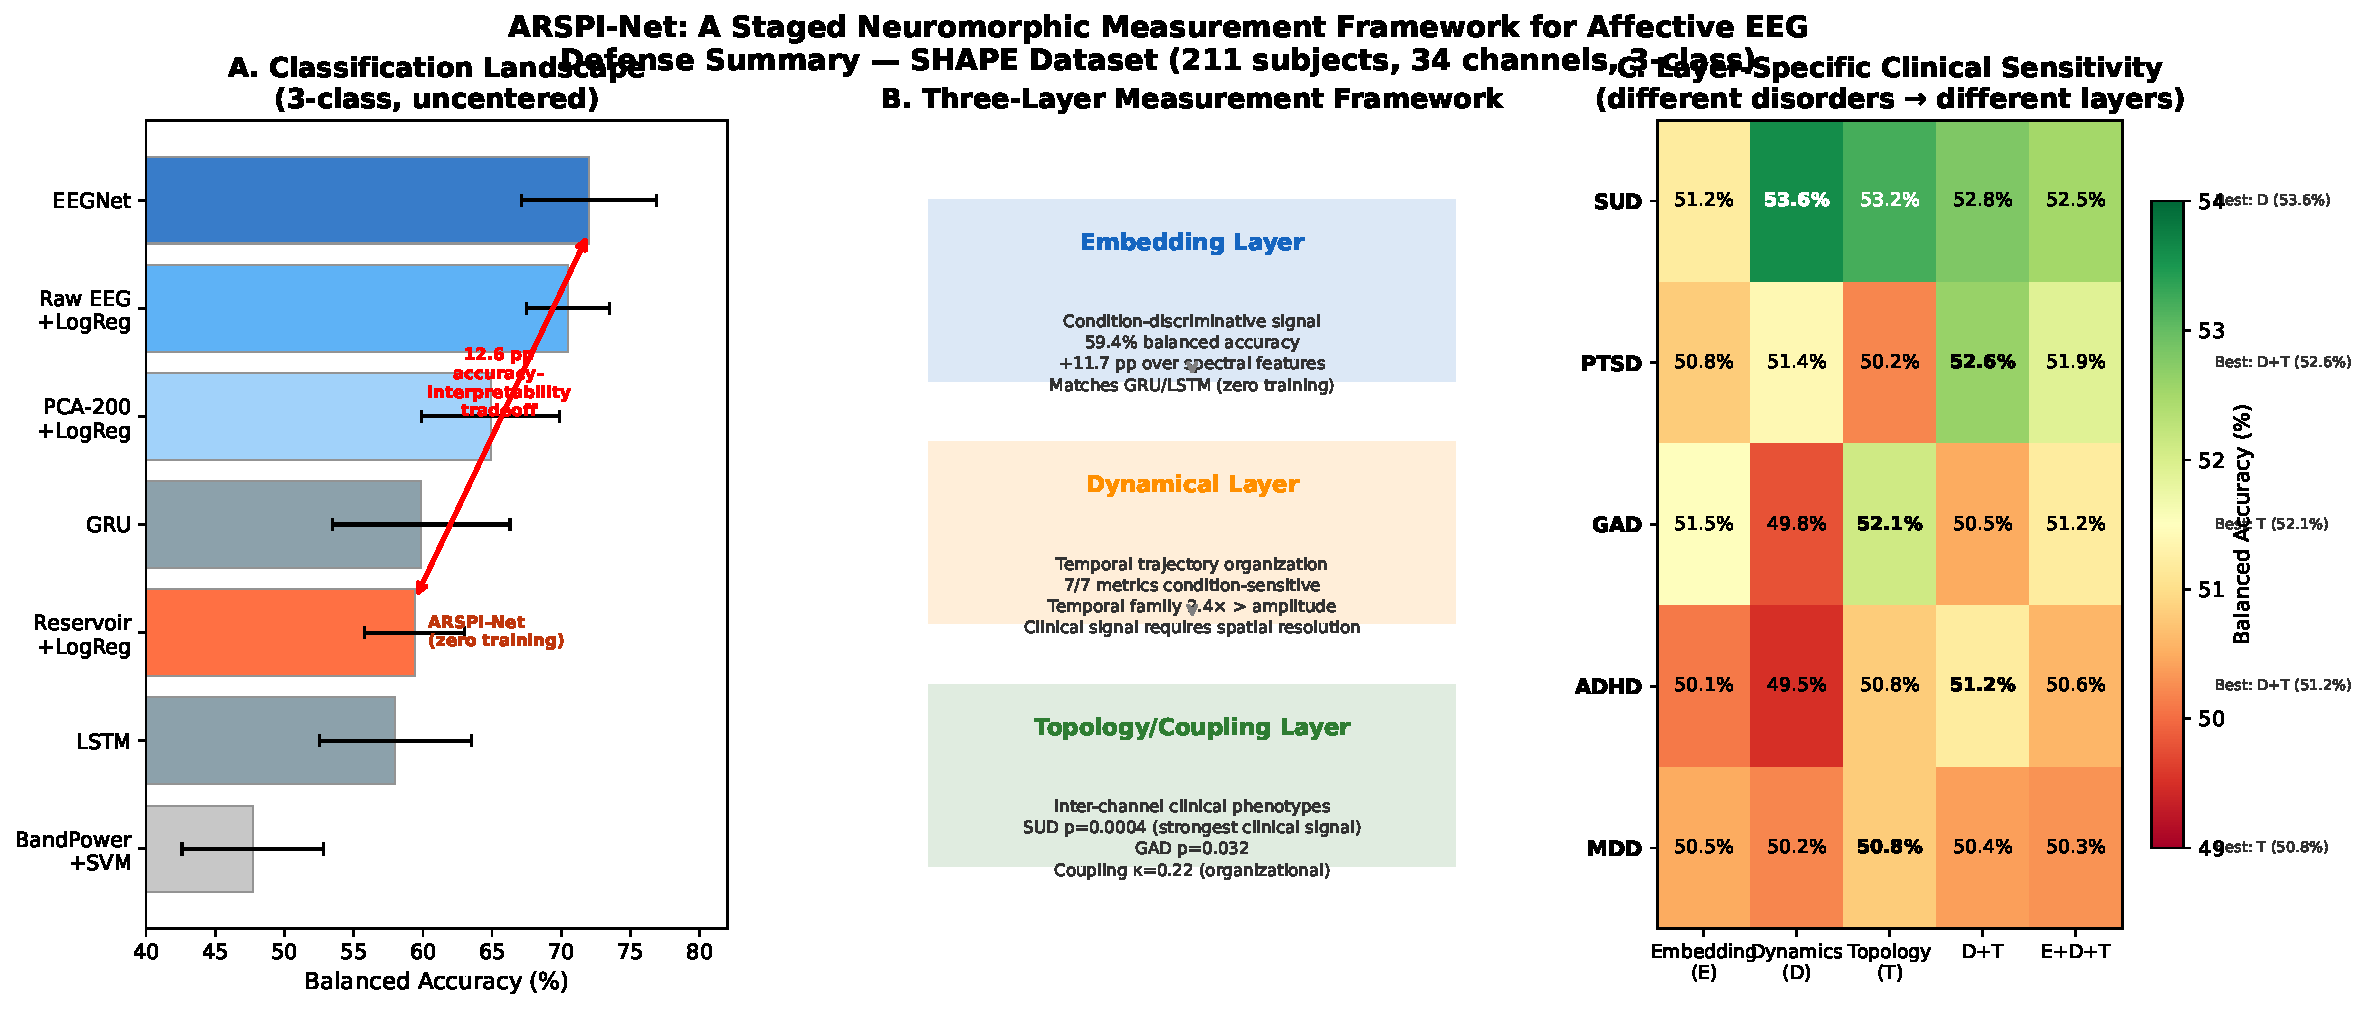
\includegraphics[height=0.78\textheight]{pictures/conclusion/fig_defense_summary.pdf}
\end{frame}


\section{Appendix --- Defense Audit Diagnostics}

\begin{frame}{Appendix --- Defense audit: raw diagnostics overview}
  \vspace{0.6em}
  Raw diagnostic strips backing the new measured-operator slides
  (Exp A--D), plus the figure-to-source backup index for the
  dissertation anchor map (AM).
  \vspace{0.6em}
  \begin{itemize}\small
    \item Exp A: eigenspectrum of $W$; Benettin sample trajectories;
          per-trial $\lambda_1$ scatter.
    \item Exp B: delay embedding; per-trial FNN distribution.
    \item Exp C: input drive; state response per $\beta$; MC vs.\ $\tau$.
    \item Exp D: feature layout; class-label distribution; observed
          vs.\ null example.
    \item AM: figure-to-source backup index.
  \end{itemize}
\end{frame}

\begin{frame}{Appendix --- Exp A raw: eigenspectrum of $W$}
  \centering
  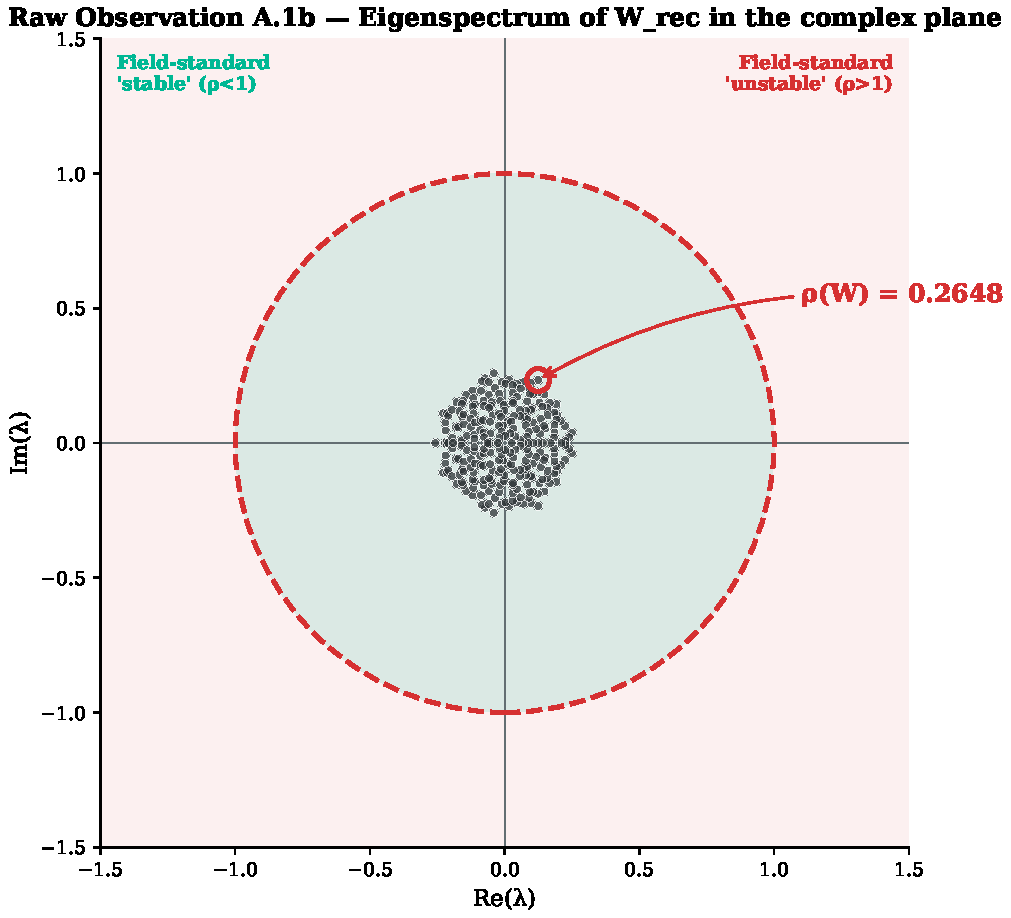
\includegraphics[height=0.78\textheight]{pictures/defense_audit/rawA_1b_eigenspectrum.pdf}
\end{frame}

\begin{frame}{Appendix --- Exp A raw: Benettin sample trajectories}
  \centering
  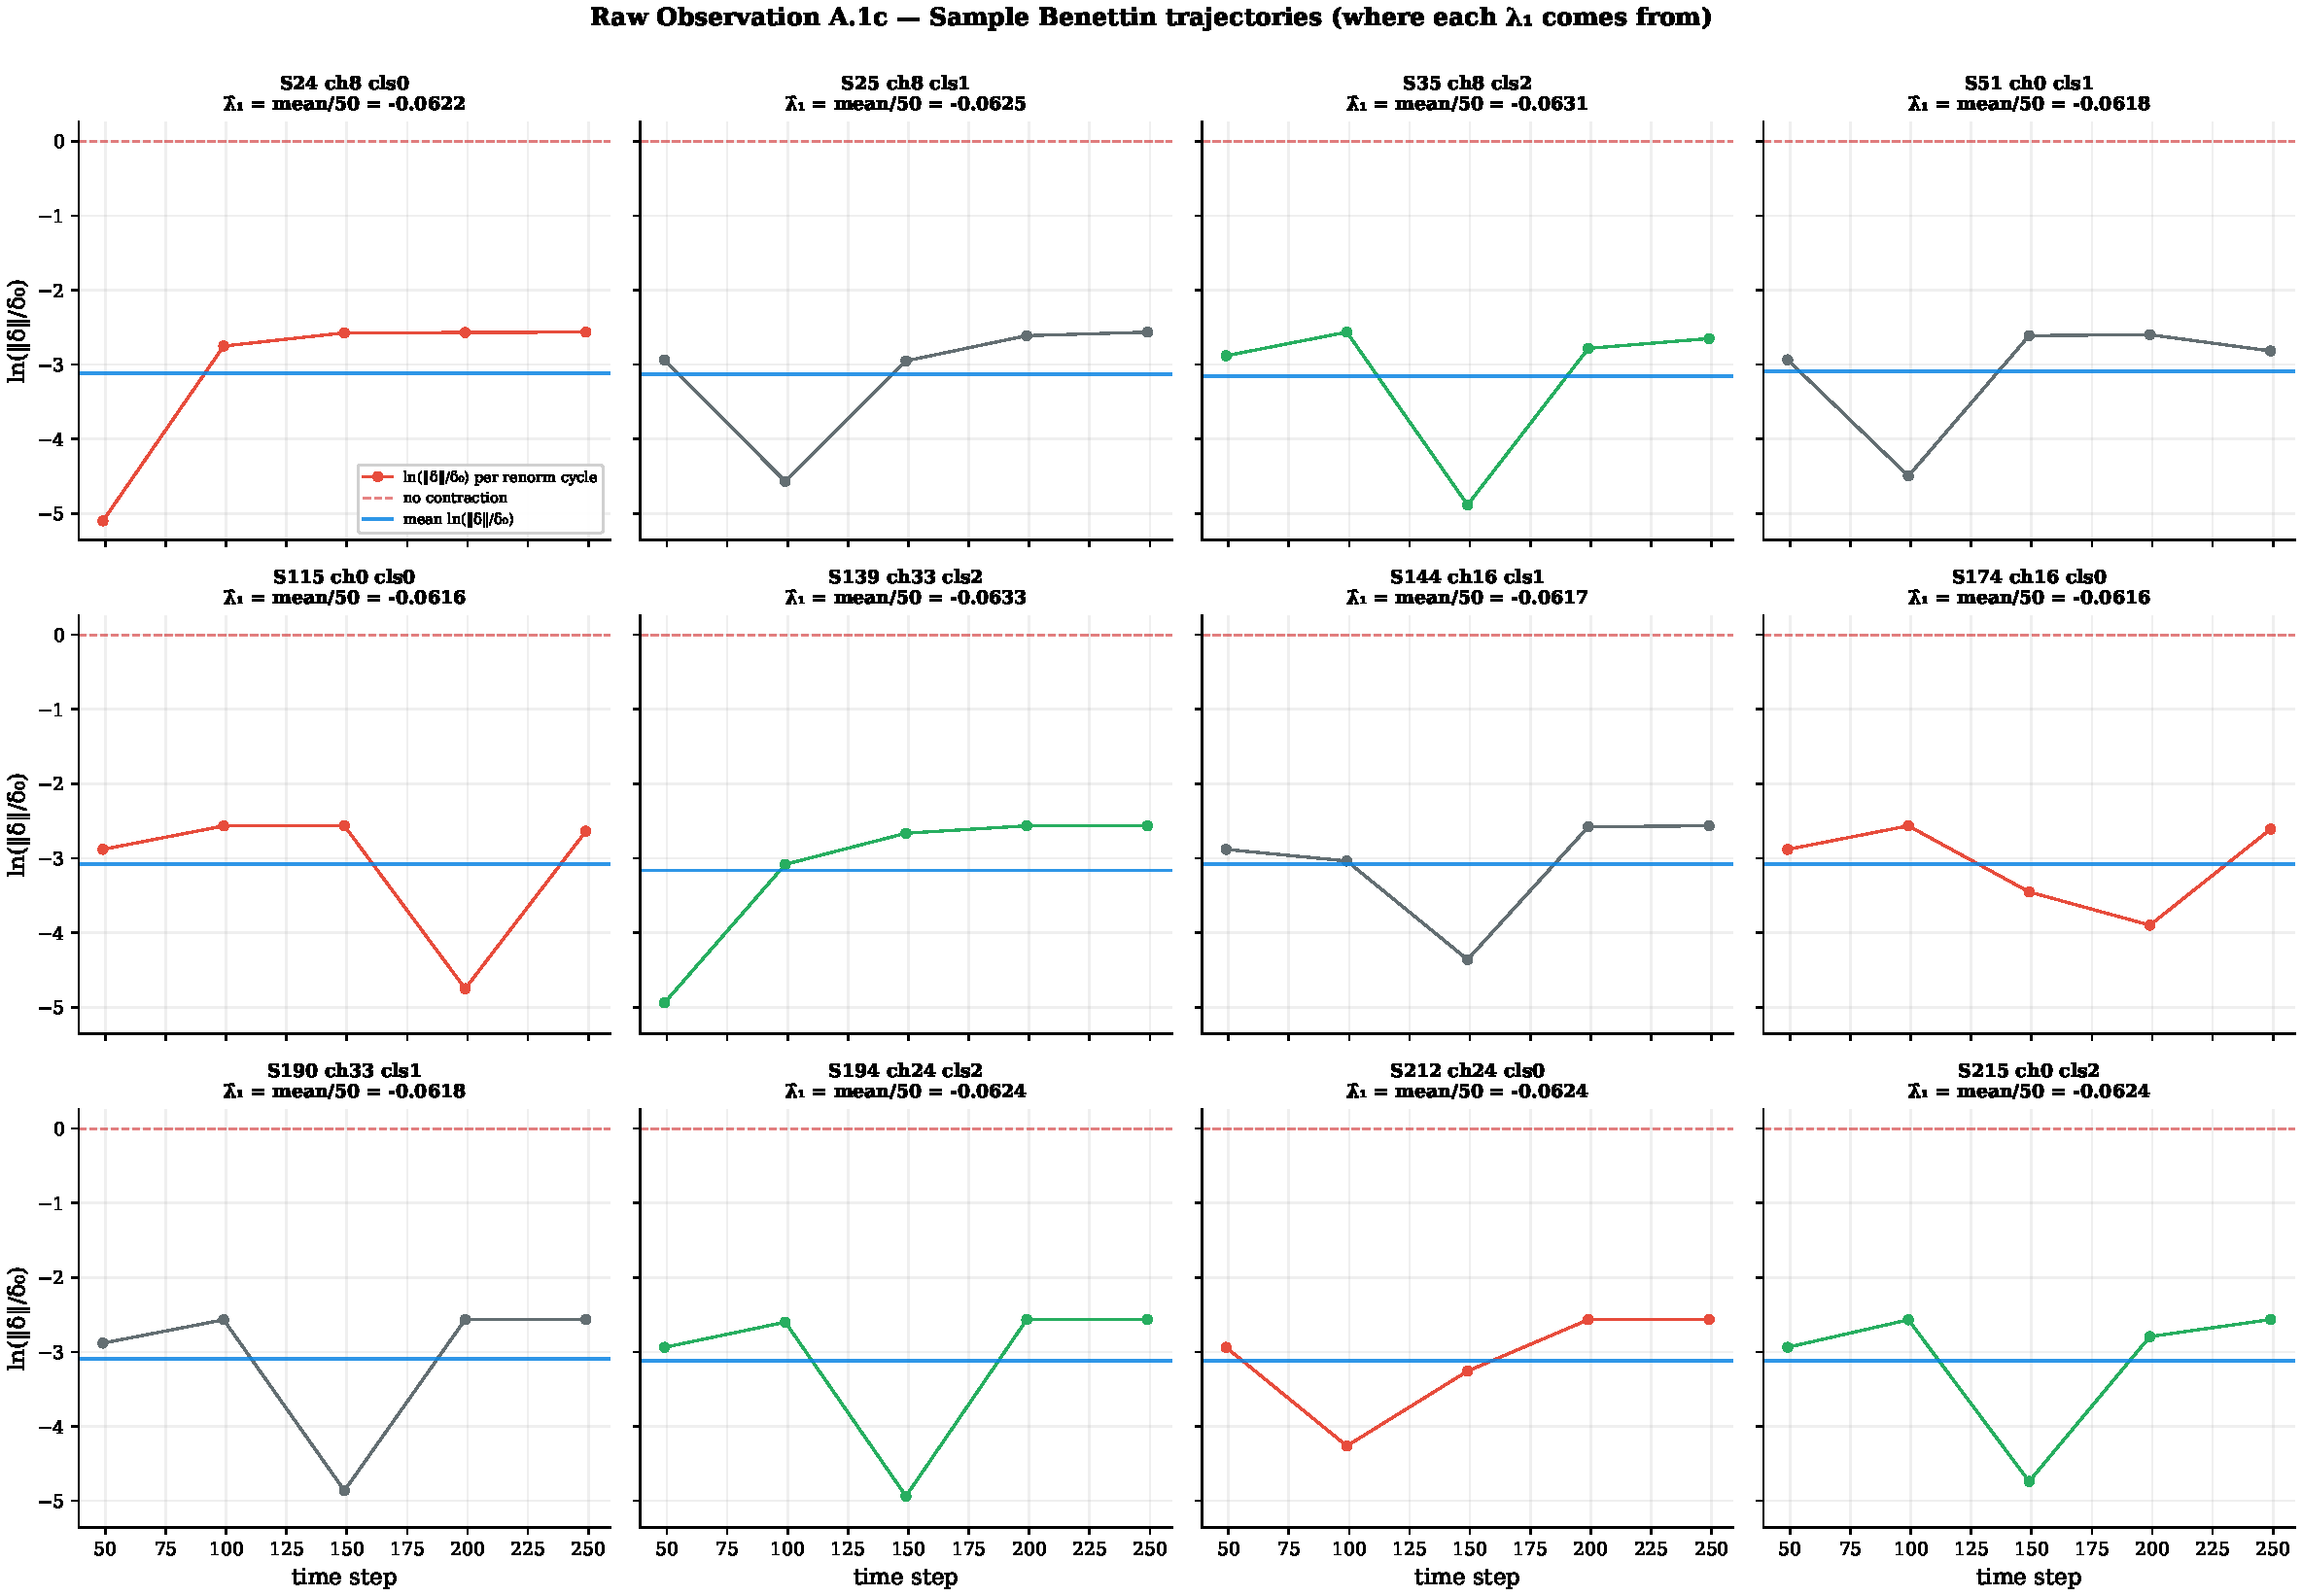
\includegraphics[height=0.78\textheight]{pictures/defense_audit/rawA_1c_benettin_sample_trajectories.pdf}
\end{frame}

\begin{frame}{Appendix --- Exp A raw: per-trial $\lambda_1$ scatter}
  \centering
  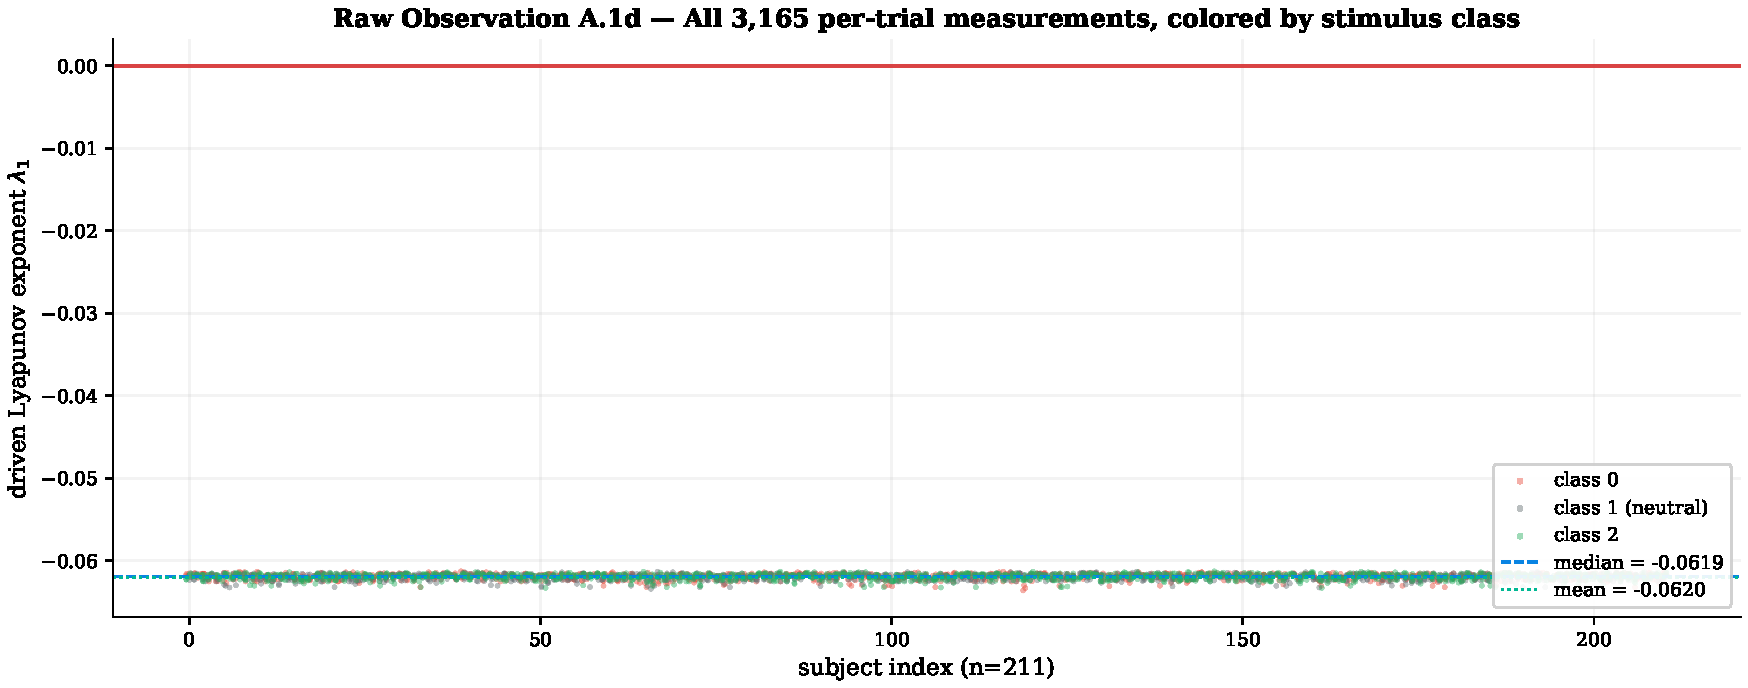
\includegraphics[height=0.78\textheight]{pictures/defense_audit/rawA_1d_per_trial_lambda_scatter.pdf}
\end{frame}

\begin{frame}{Appendix --- Exp B raw: delay embedding}
  \centering
  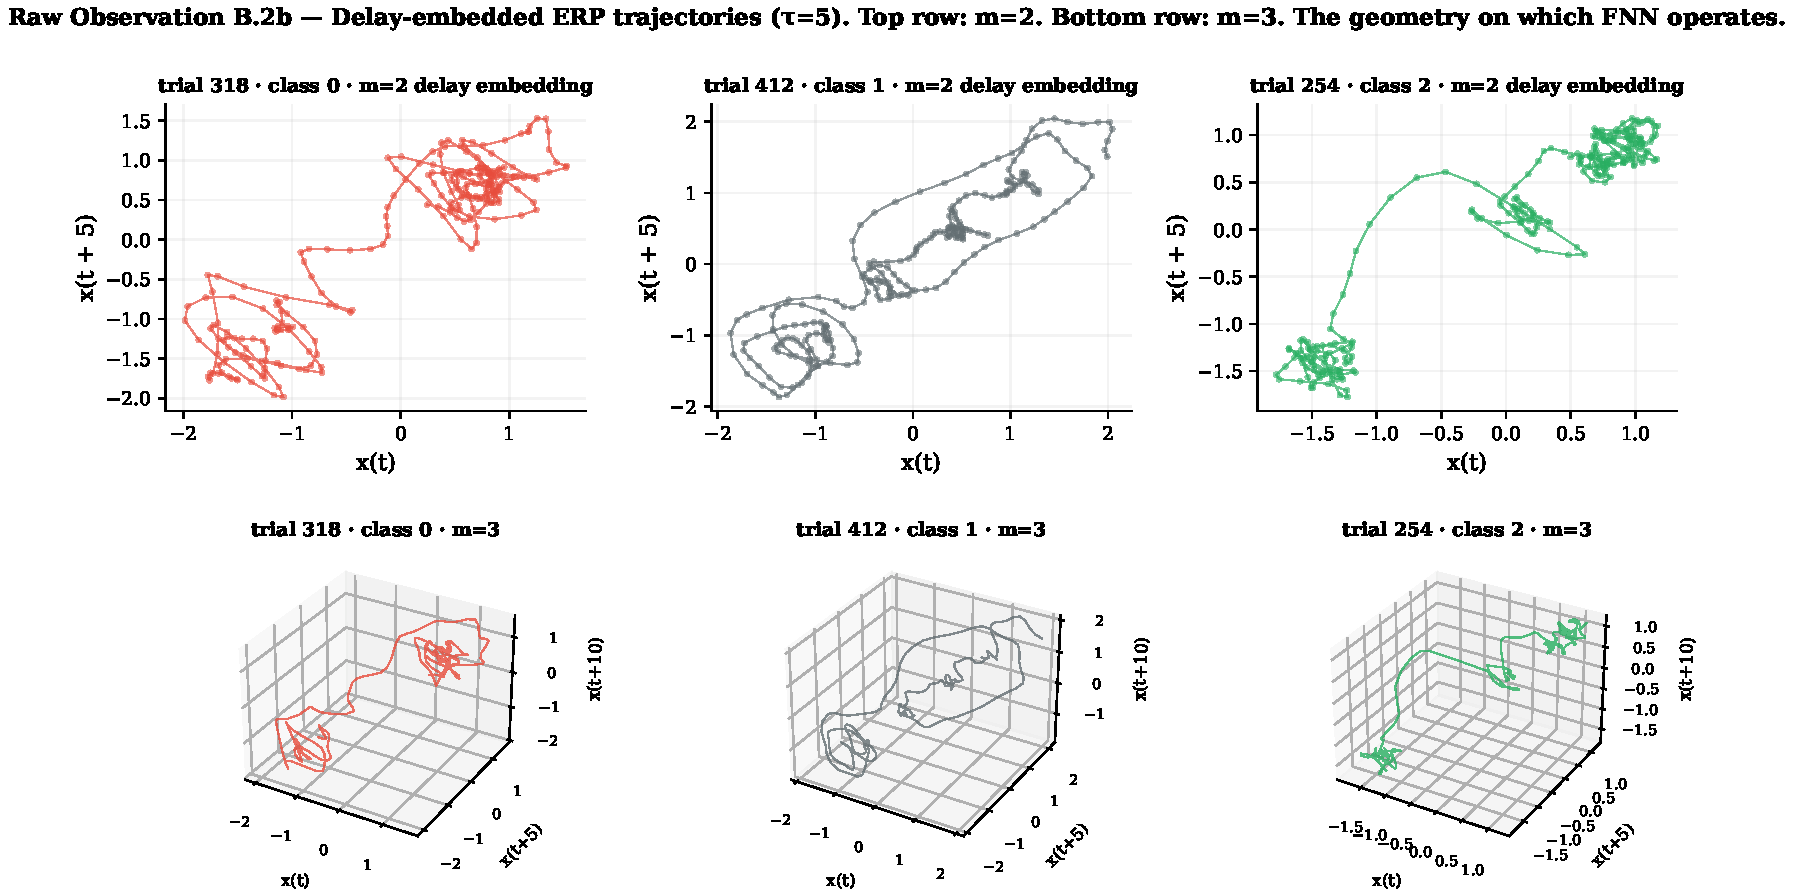
\includegraphics[height=0.78\textheight]{pictures/defense_audit/rawB_2b_delay_embedding.pdf}
\end{frame}

\begin{frame}{Appendix --- Exp B raw: per-trial FNN distribution}
  \centering
  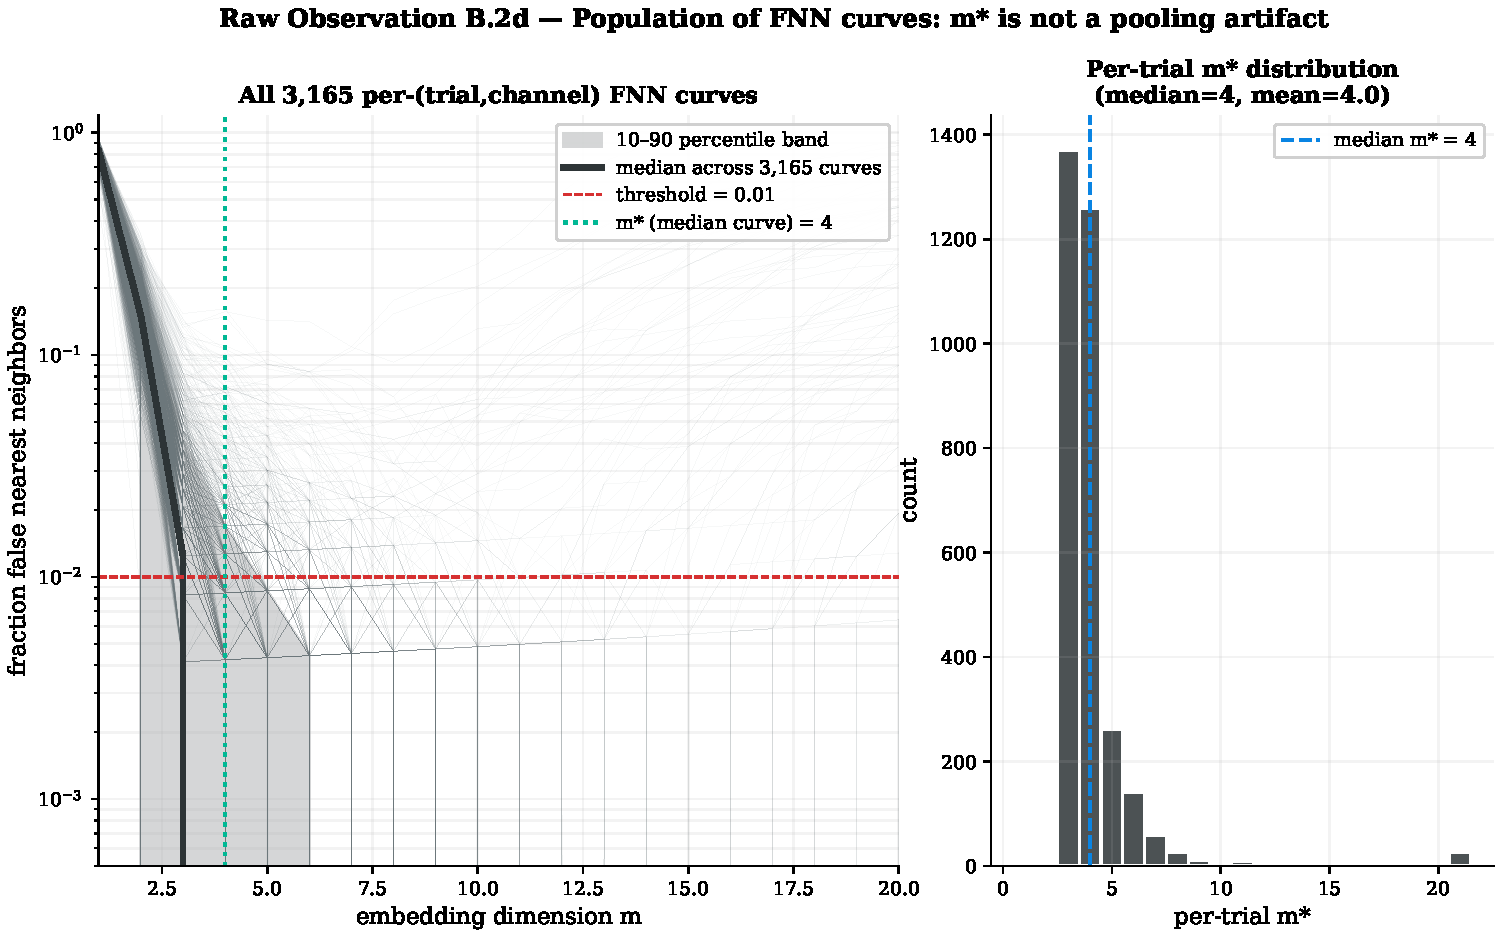
\includegraphics[height=0.78\textheight]{pictures/defense_audit/rawB_2d_per_trial_fnn.pdf}
\end{frame}

\begin{frame}{Appendix --- Exp C raw: input drive}
  \centering
  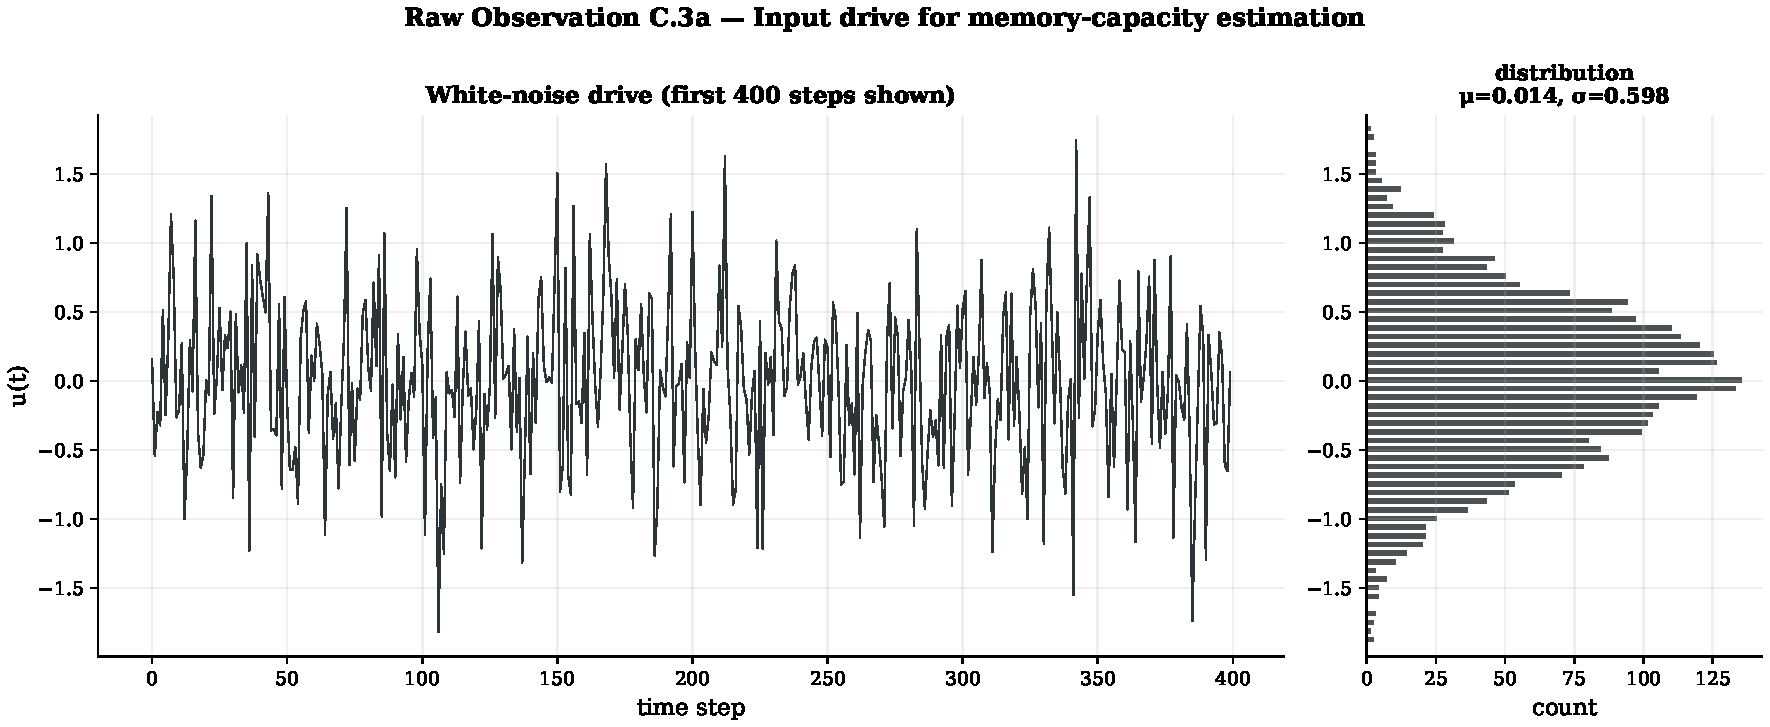
\includegraphics[height=0.78\textheight]{pictures/defense_audit/rawC_3a_input_drive.pdf}
\end{frame}

\begin{frame}{Appendix --- Exp C raw: state response per $\beta$}
  \centering
  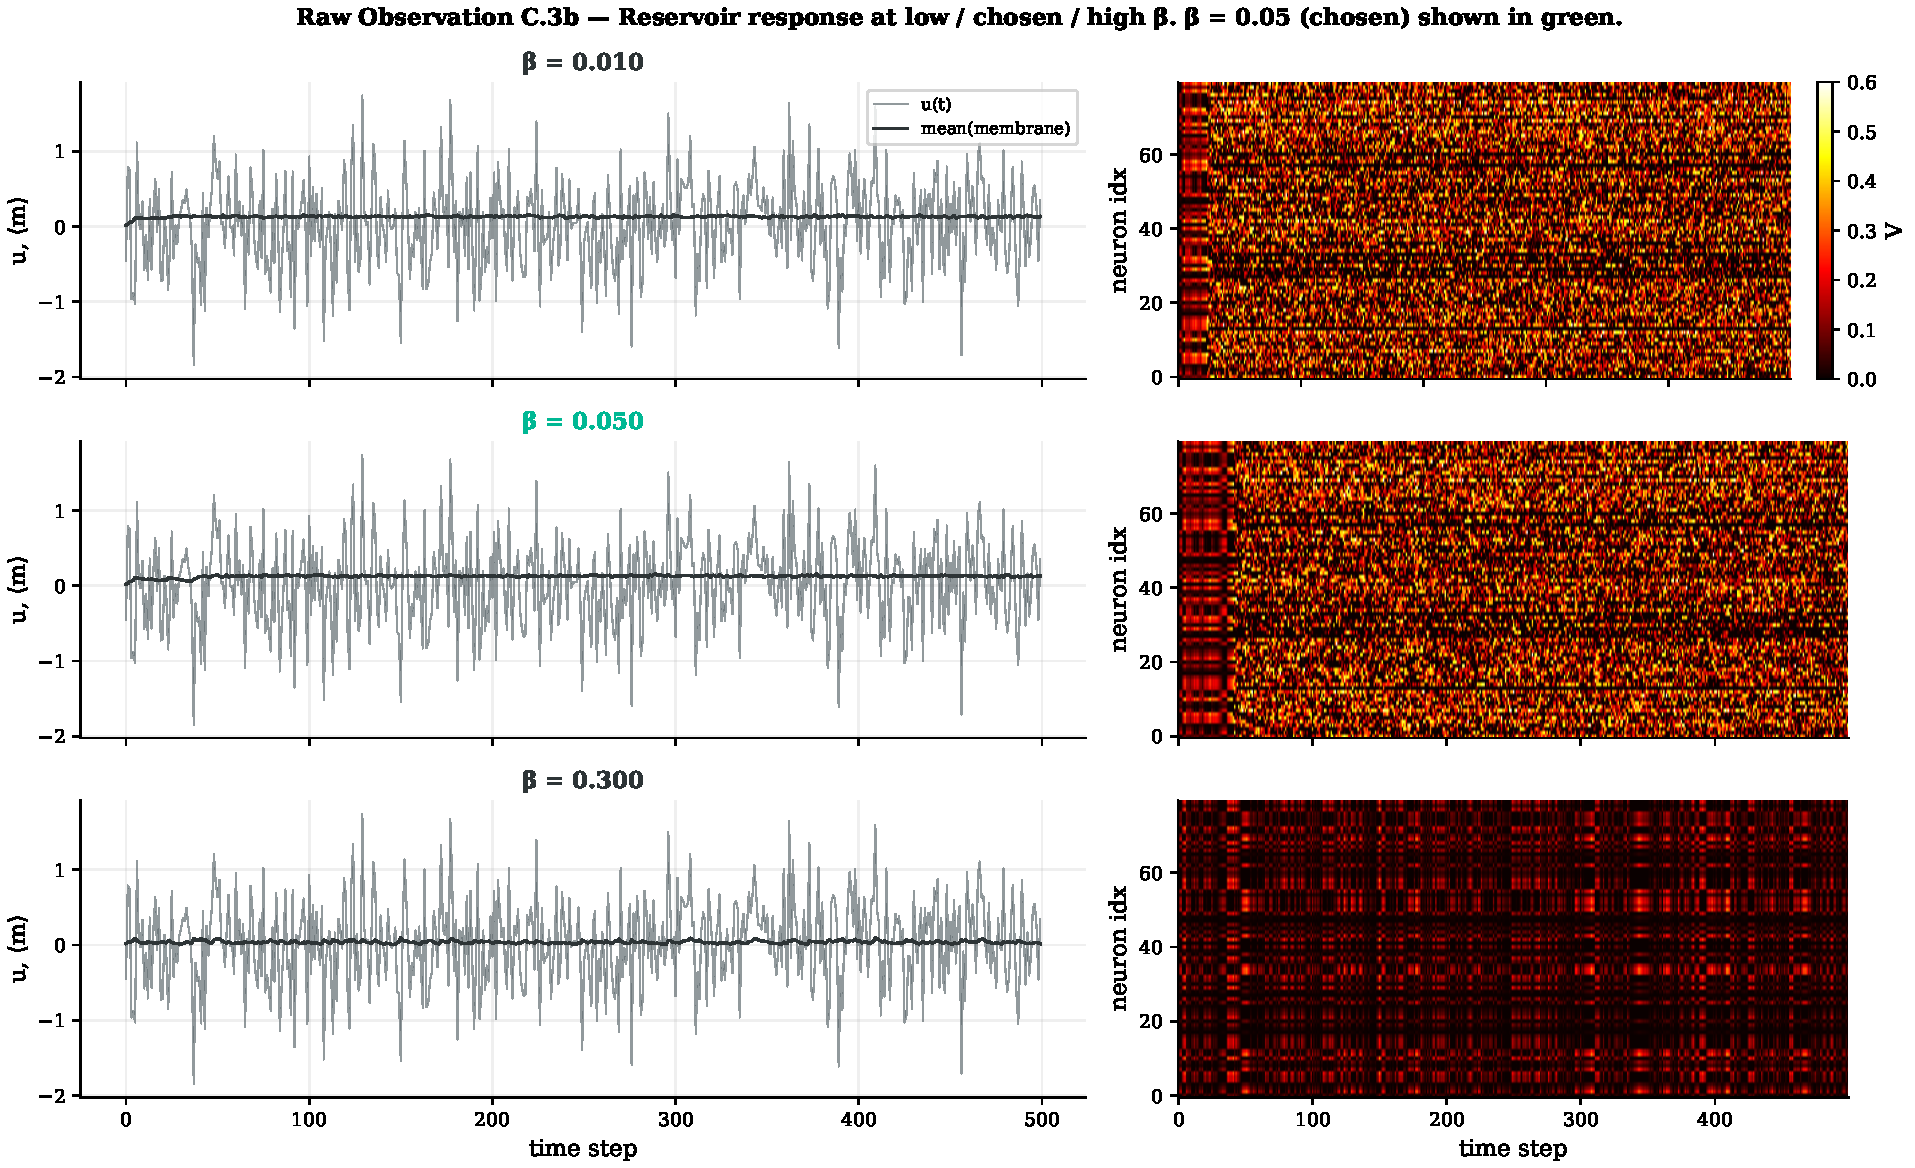
\includegraphics[height=0.78\textheight]{pictures/defense_audit/rawC_3b_state_response_per_beta.pdf}
\end{frame}

\begin{frame}{Appendix --- Exp C raw: memory capacity vs.\ $\tau$}
  \centering
  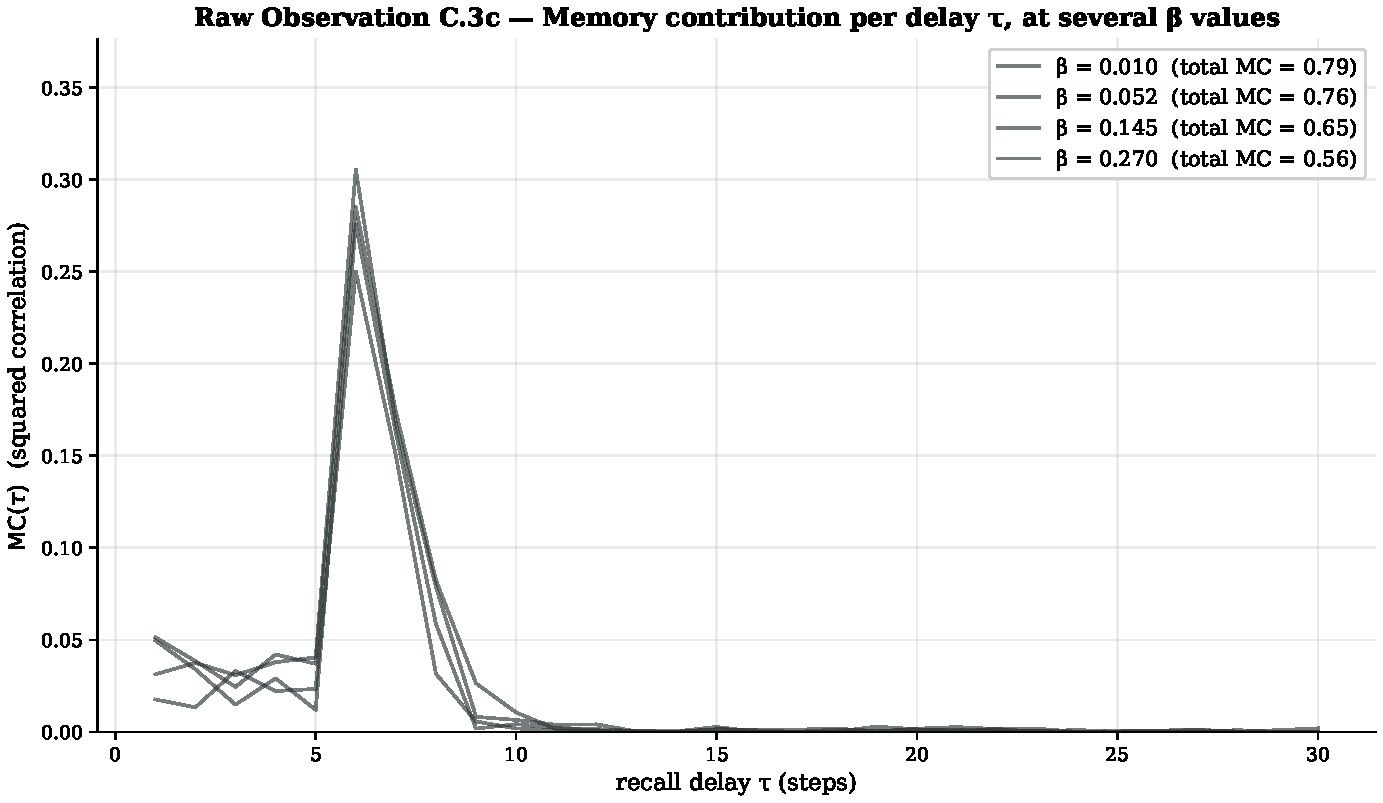
\includegraphics[height=0.78\textheight]{pictures/defense_audit/rawC_3c_mc_vs_tau.pdf}
\end{frame}

\begin{frame}{Appendix --- Exp D raw: feature layout}
  \centering
  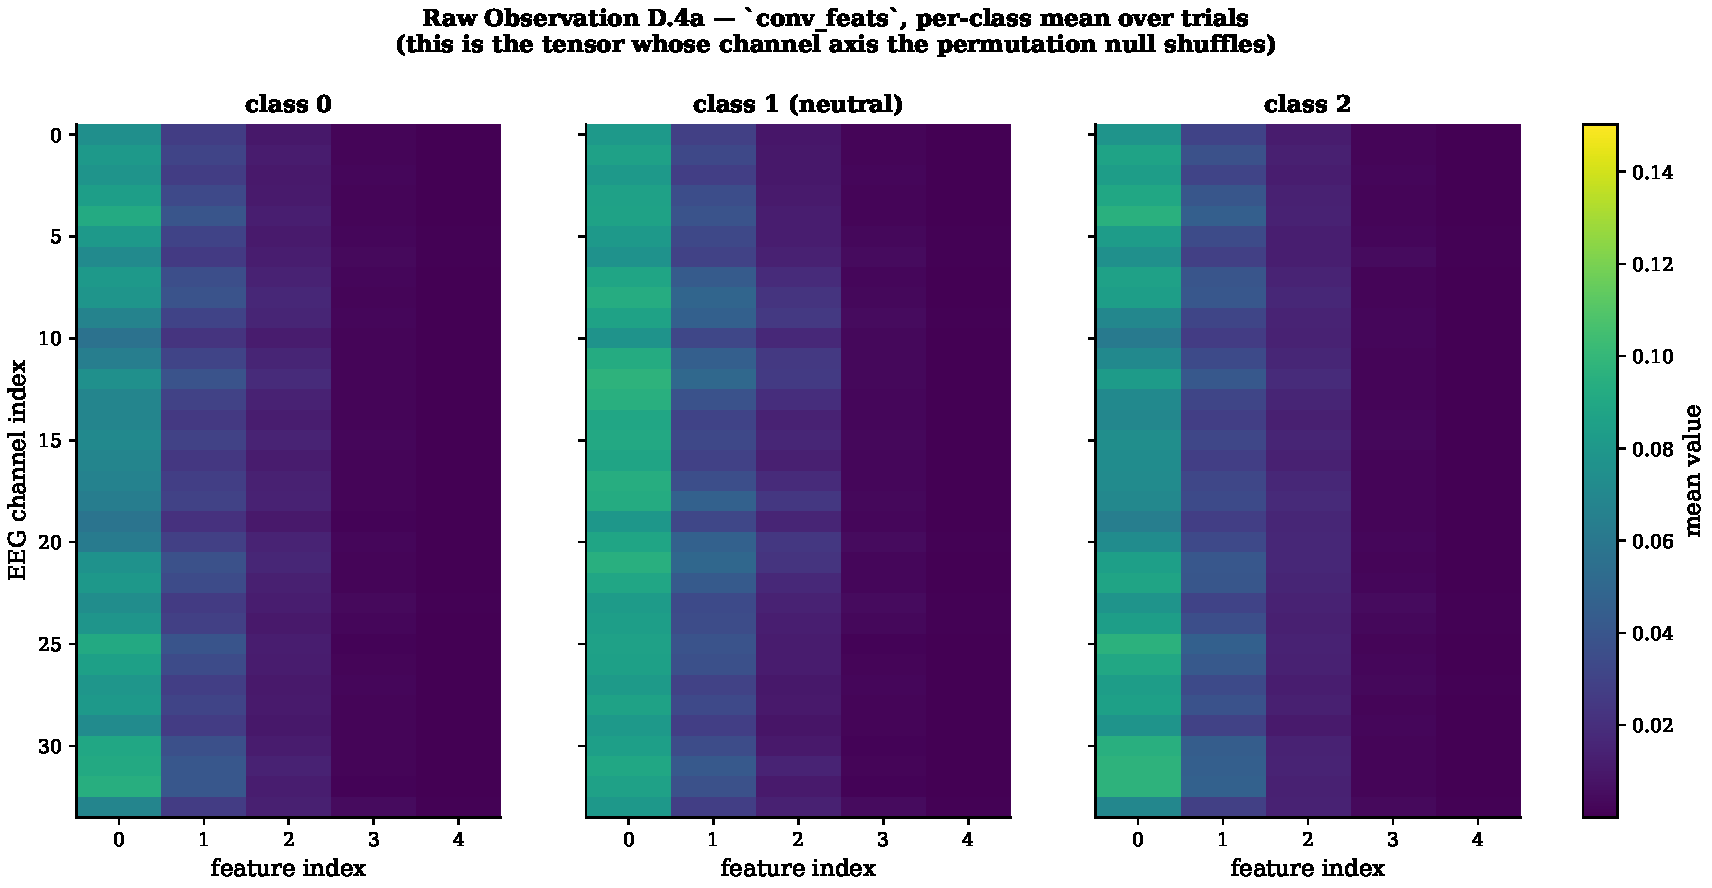
\includegraphics[height=0.78\textheight]{pictures/defense_audit/rawD_4a_feature_layout.pdf}
\end{frame}

\begin{frame}{Appendix --- Exp D raw: class-label distribution}
  \centering
  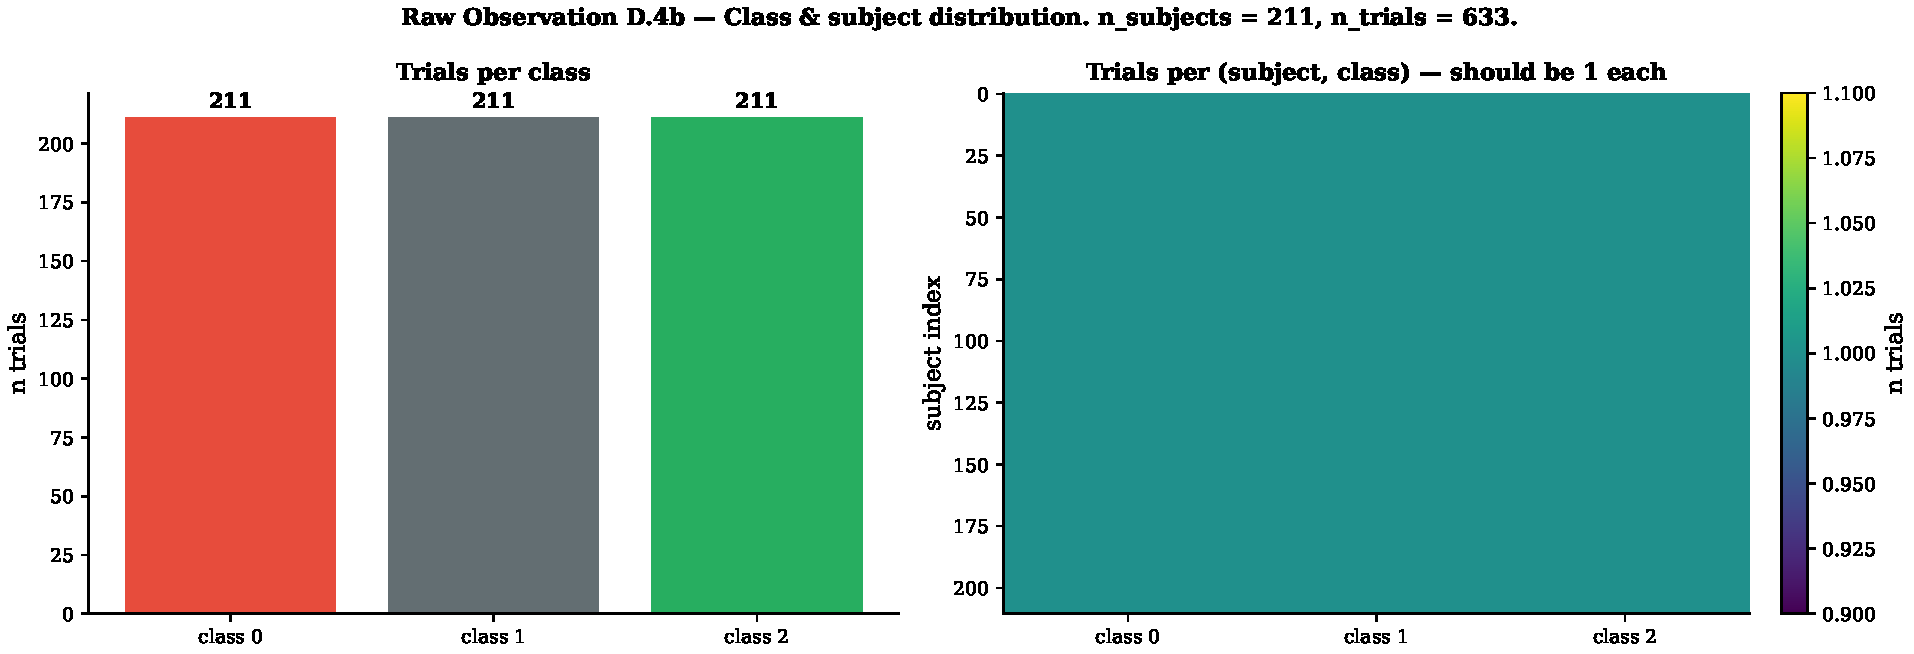
\includegraphics[height=0.78\textheight]{pictures/defense_audit/rawD_4b_class_label_distribution.pdf}
\end{frame}

\begin{frame}{Appendix --- Exp D raw: observed vs.\ null example}
  \centering
  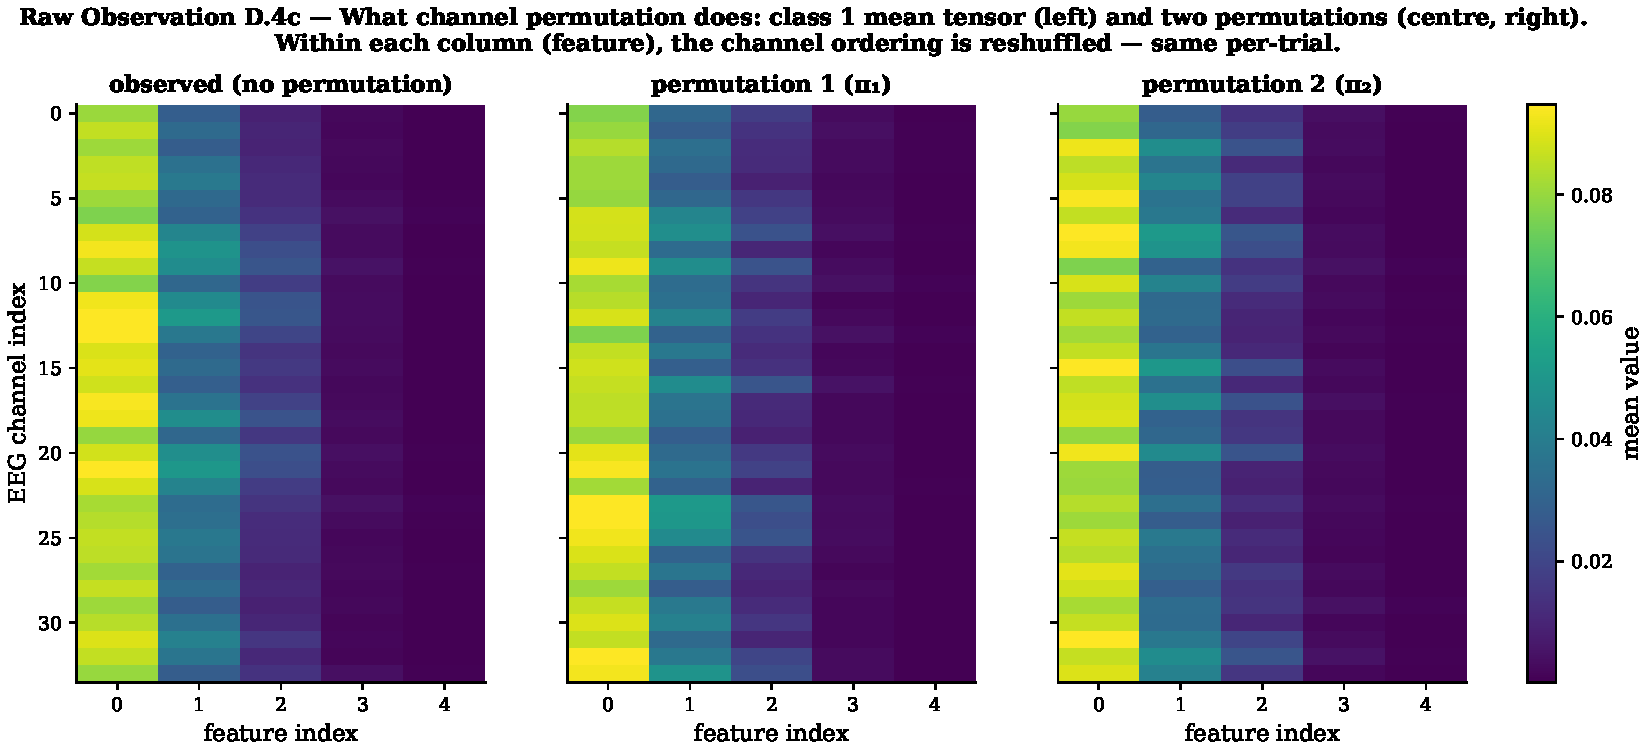
\includegraphics[height=0.78\textheight]{pictures/defense_audit/rawD_4c_observed_vs_null_example.pdf}
\end{frame}

\begin{frame}{Appendix --- AM: figure-to-source backup index}
  \centering
  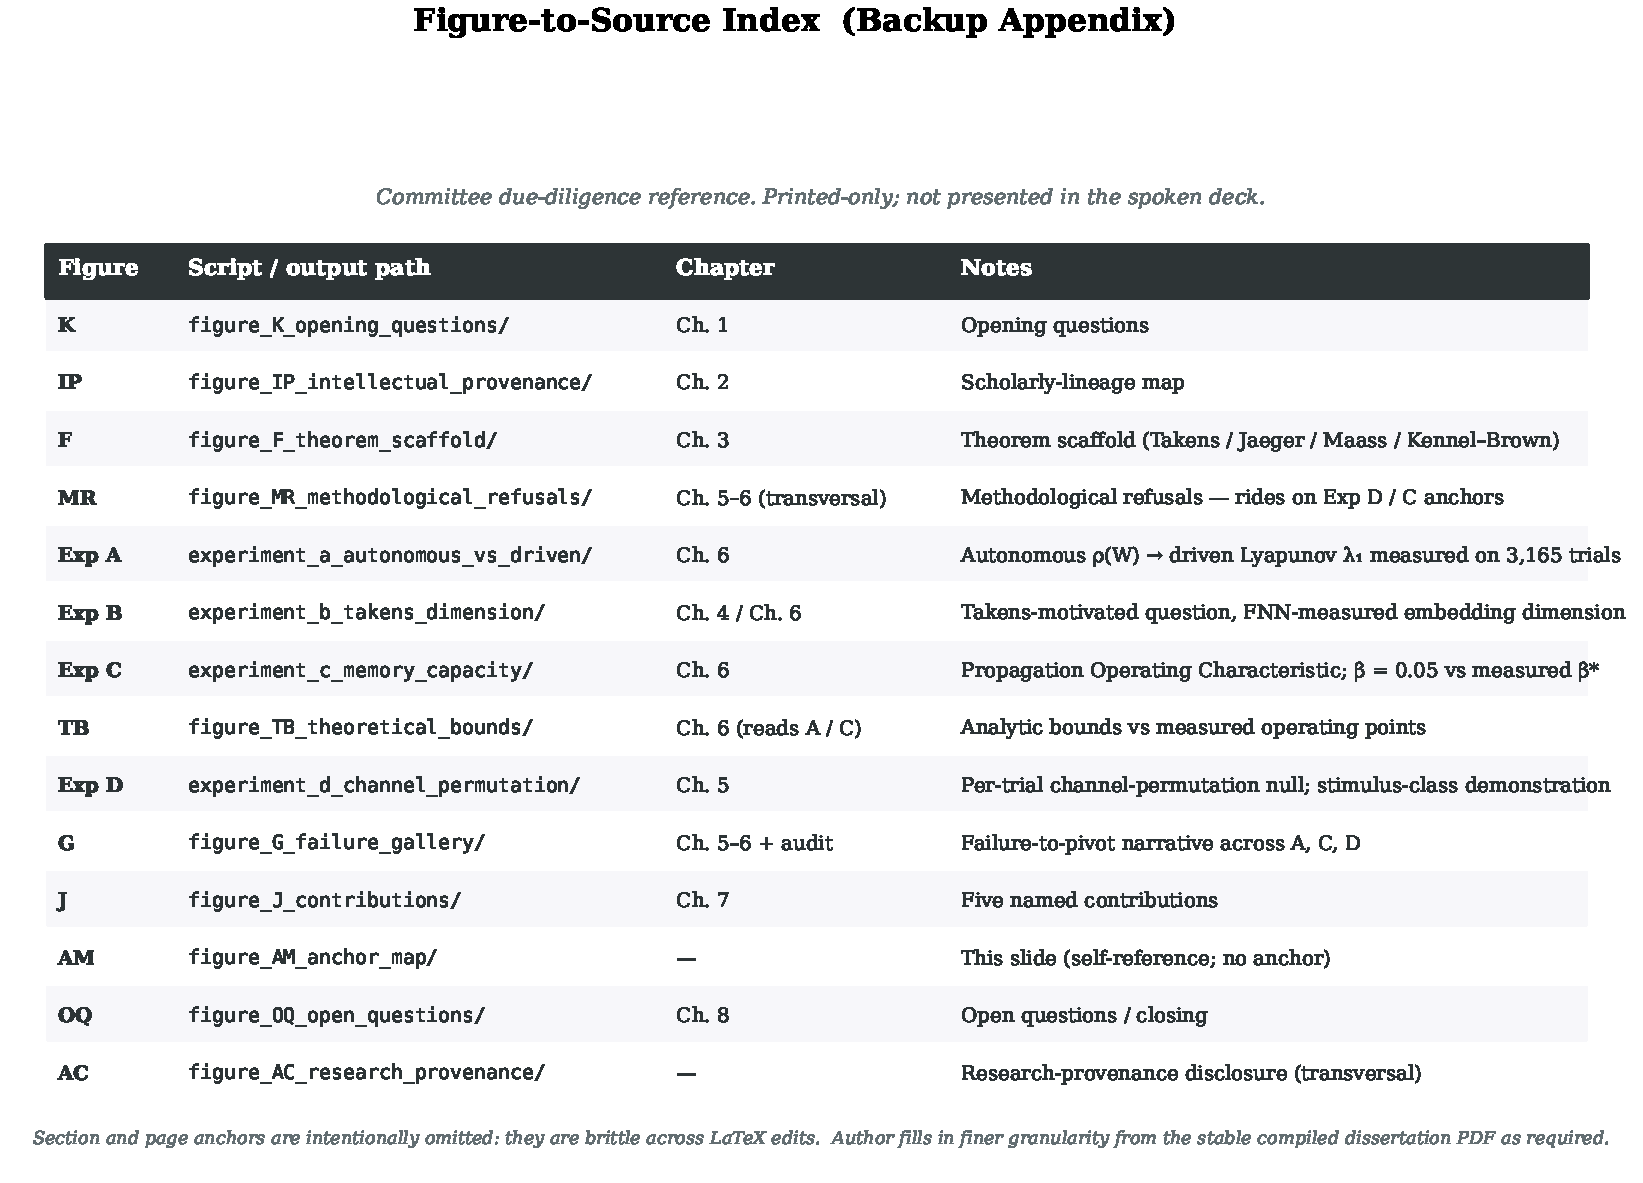
\includegraphics[width=\textwidth,height=0.82\textheight,keepaspectratio]{pictures/defense_audit/figAM_source_index.pdf}
\end{frame}

\end{document}
